\documentclass[../document.tex]{subfiles}
\begin{document}
\chapter{Interpretability}
\label{chap: interpretability}
In this section, we interpret MicroResNet7x7-SE's predictions using different techniques to test its ability to properly estimate traversability by classifying ground patches. We highlight its strength, robustness to understand its limitations. We evaluated the quality of our traversability estimator with different methodology. First, we showed that the model has correctly learned grounds' features and was able to separable terrains based on them. Second, we utilized the test dataset to visualize the most traversable, the lest traversable and the misclassified patches.  Utilizing a special method, we determined that the model always looked at the correct features in the ground even if when it fails. Lastly, we crafted several patches with different unique features, such as walls, bumps, etc, to test the robustness of the model by comparing its predictions to the real data gathered from the simulator. 
\section{Features separability}
\label{sec: features-separability}
In general, convolutional neural networks learn to encode images by applying filters of increasing size at each layer. Usually, the first layers learn basic features, such as edges, while the final one encodes complex shapes. The outputs in the final convolution layer are usually referred to as \emph{features space}, consequently, a feature vector is just the output of the last layer for a given image. Those last features are combined and mapped to the correct classes by one or more fully connected layers. Lee et al. \cite{deepbelief} have visualized the features learned by the first and last layers. Figure \ref 
The following image help to visualize the different features learned at each layer for network trained to classify images. This is visualize in figure \ref{layers-features} where there are the low level features (down) and the high level features (up) for four different classes, faces, cars, elephants and chairs, learned by a convolution neural network.
\begin{figure} [htbp]
    \centering
    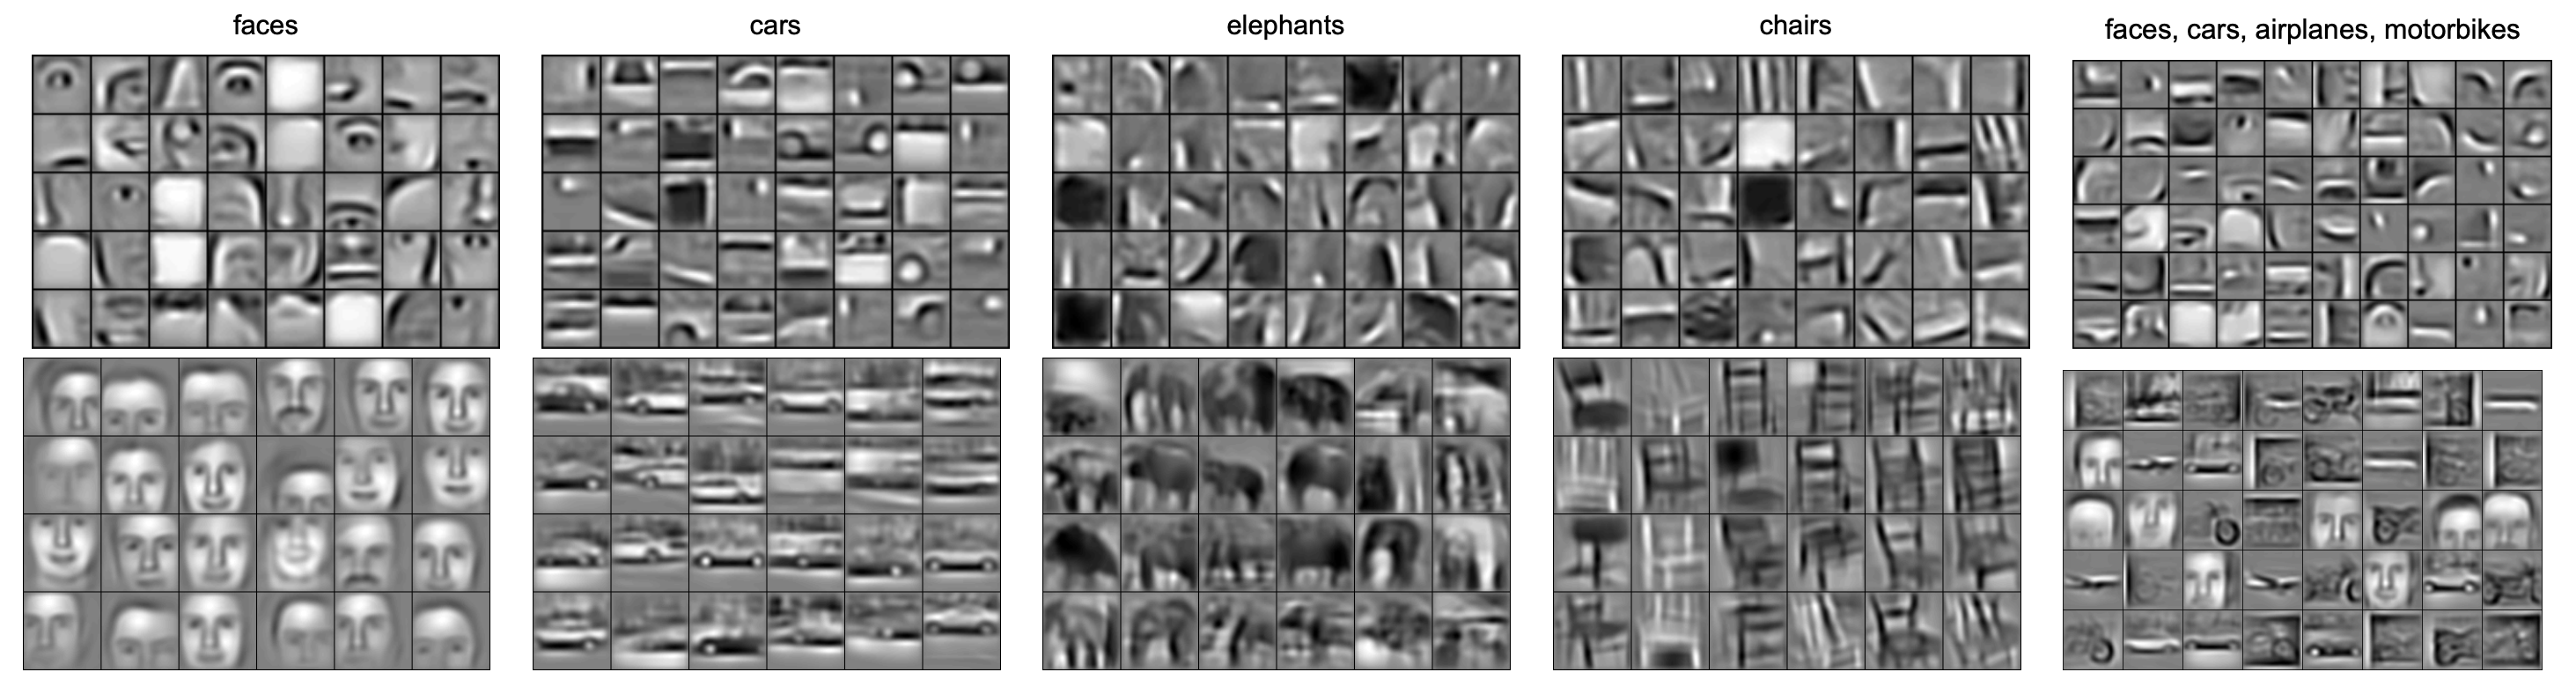
\includegraphics[width=\linewidth]{../img/5/deep_belief.png}
    \caption{Figure from Lee et al. \cite{deepbelief} paper where they showed for fours different classes the low-level features (up) and the high-level features (down) learned by a convolution neural network.}
    \label{fig : layers-features}
\end{figure}
So, a correctly trained network should be able to separate the inputs features based on the predicted classes. Intuitively, given two classes $\mathcal{A}$ and $\mathcal{B}$, for example, \emph{chairs} and \emph{cars}, the high-level features for each class should not be the same, otherwise, the model may misclassify the input due to the overlap of different classes' features. For instance, if the network believes that big wheels are features of both chairs and cars then chairs may be wrongly classified as cars. Similarly, two patches have a small and big wall in front of the robot should not be mapped in the same position in the features. Because, from a traversability point of view, have different characteristic, one has a traversable wall, the other not. However, those patches are close to each other in the features space, the model could foolishly believe they are similar and belong to the same class.
One technique to discover the degree of separability is to directly visualize the features vectors for each class. In our case,  MicroResNet7x7-SE, maps inputs to a $128$ dimensional feature space.  Since, we cannot directly visualize such highg dimension space, we reduced the feature vectors to a two-dimension space by applying Principle Analysis Component (PCA) \cite{pca}. We investigated the features space of the model both in the train and test set.

\subsection{Features space of the train set}
The following figures shows the features of $11$K images sampled from the train set labeled with their classes, \emph{traversable} and \emph{not traversable}. 
\begin{figure} [htbp]
    \centering
    \begin{subfigure}[b]{1\textwidth}
        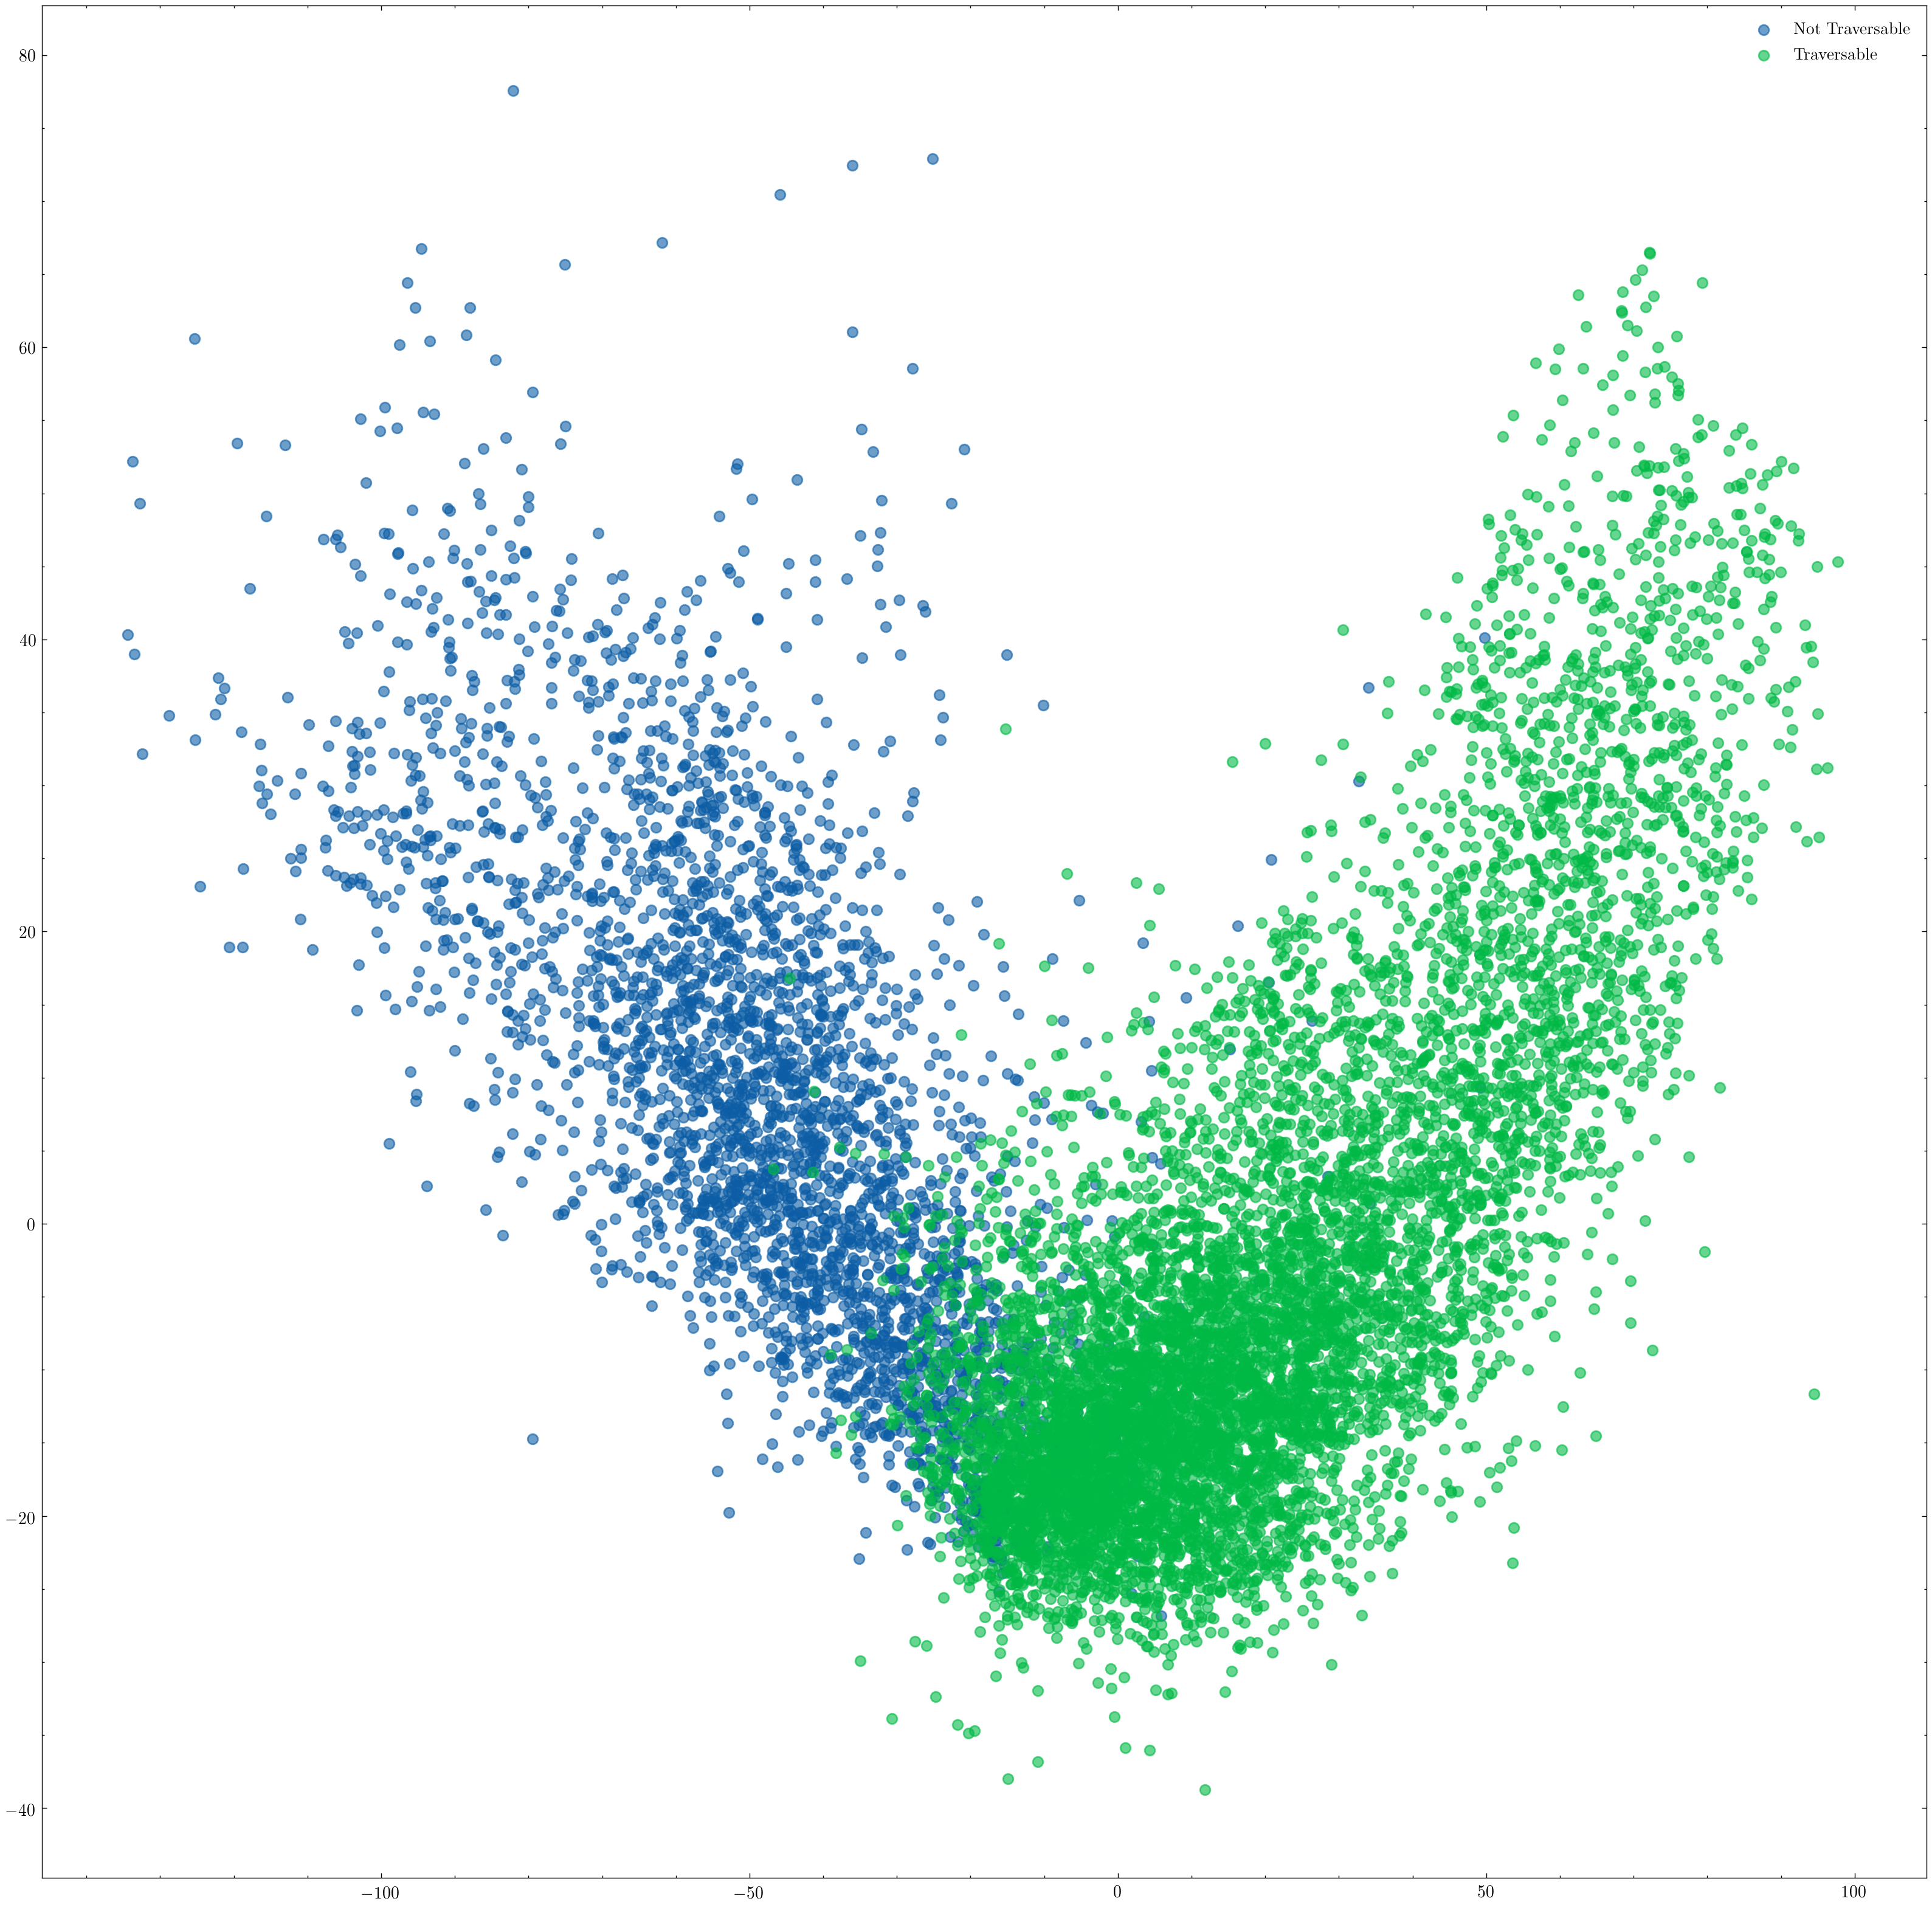
\includegraphics[width=\linewidth]{../img/5/pca/pca.png}
    \end{subfigure}
    \begin{subfigure}[b]{0.48\textwidth}
        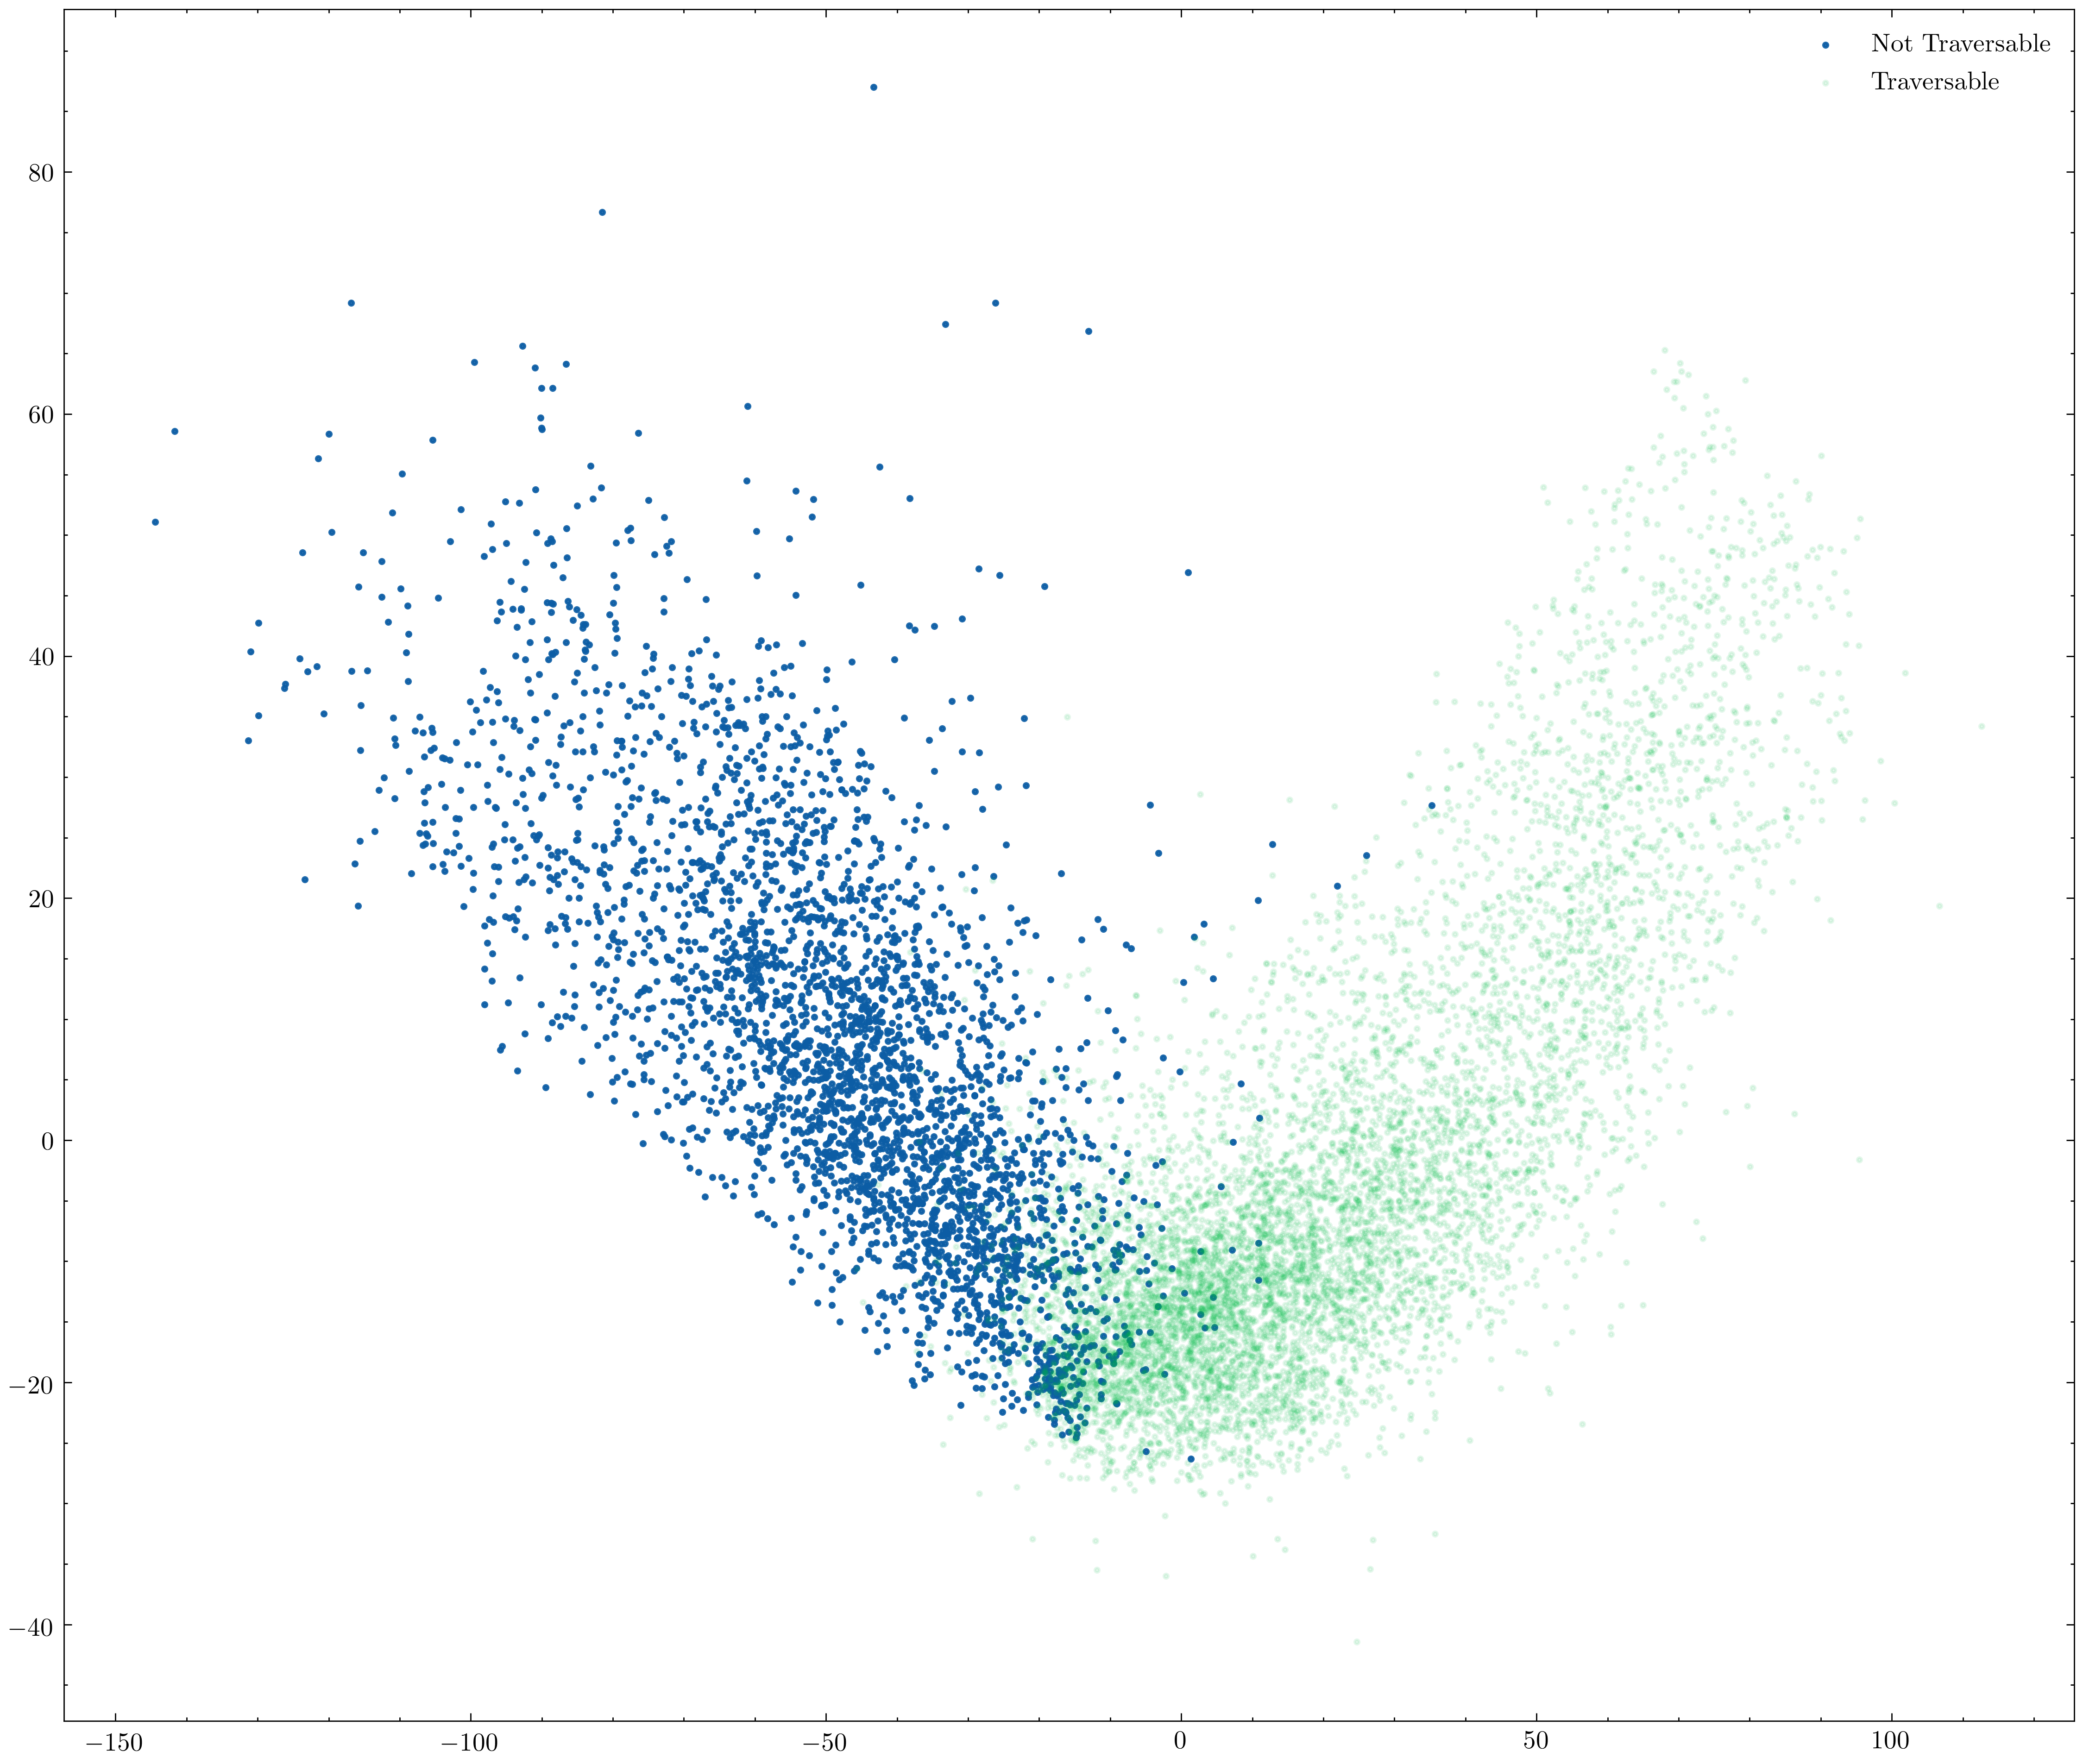
\includegraphics[width=\linewidth]{../img/5/pca/pca-0.png}
        \caption{Not Traversable}
    \end{subfigure}
    \begin{subfigure}[b]{0.48\textwidth}
        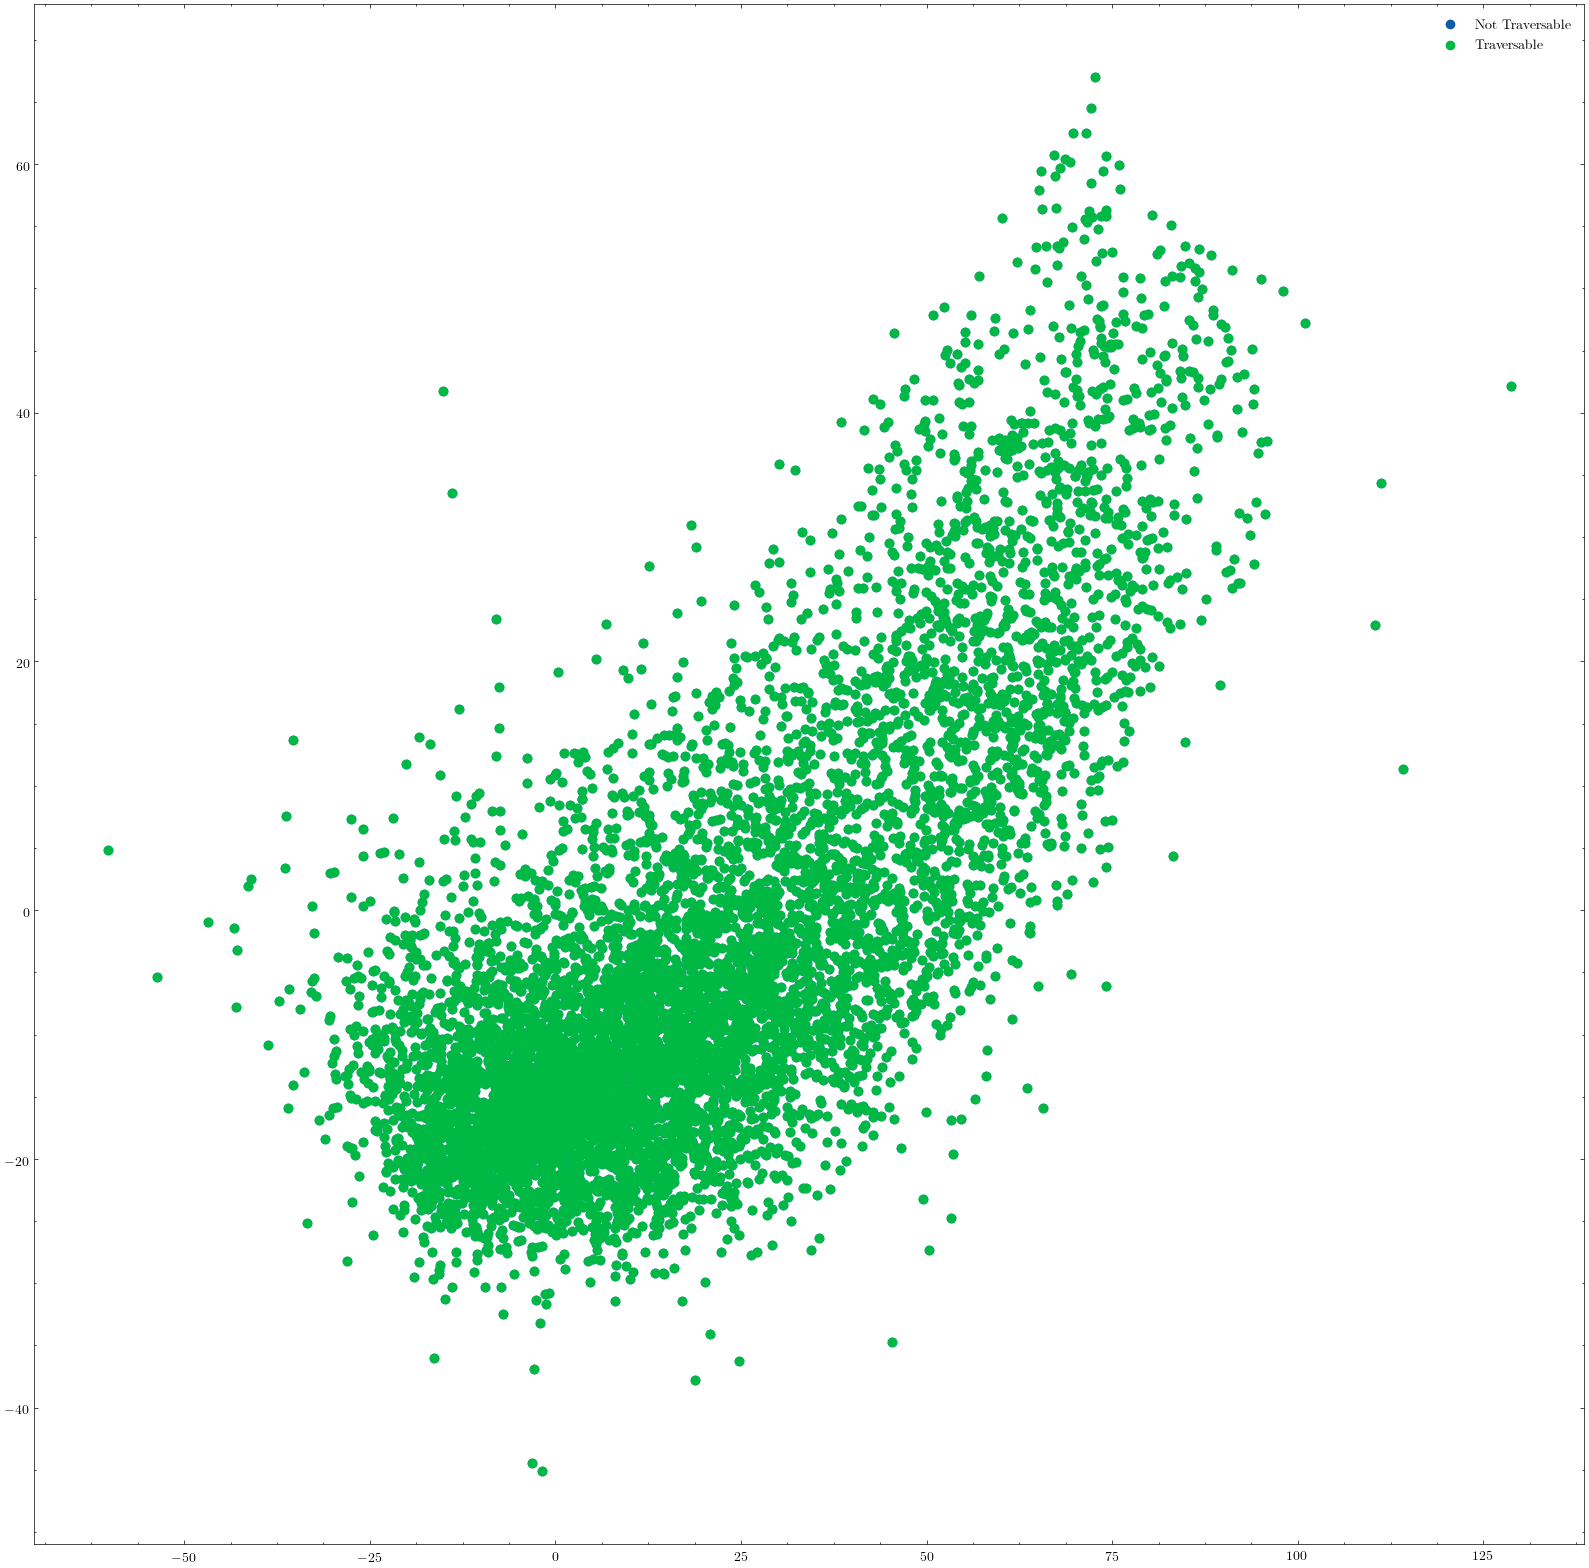
\includegraphics[width=\linewidth]{../img/5/pca/pca-1.png}
        \caption{Traversable}
    \end{subfigure}
\caption{Principal Component Analysis on the features space computed using the outputs from the last convolutional layers on the train dataset. The two point clouds are perfectly separable.}
\label{fig : pca-train-set}
\end{figure}
We can clearly recognize two main clusters based on the labels' color, one on the left and one of the right. Those points are easily separable, even by human eyes, meaning that the model was able to learn meaning features from the dataset and use to make accurate predictions. To be totally sure the center of each class' point cloud is not overlapping we plotted the density of each cluster.
\begin{figure} [htbp]
    \begin{subfigure}[b]{0.48\textwidth}
        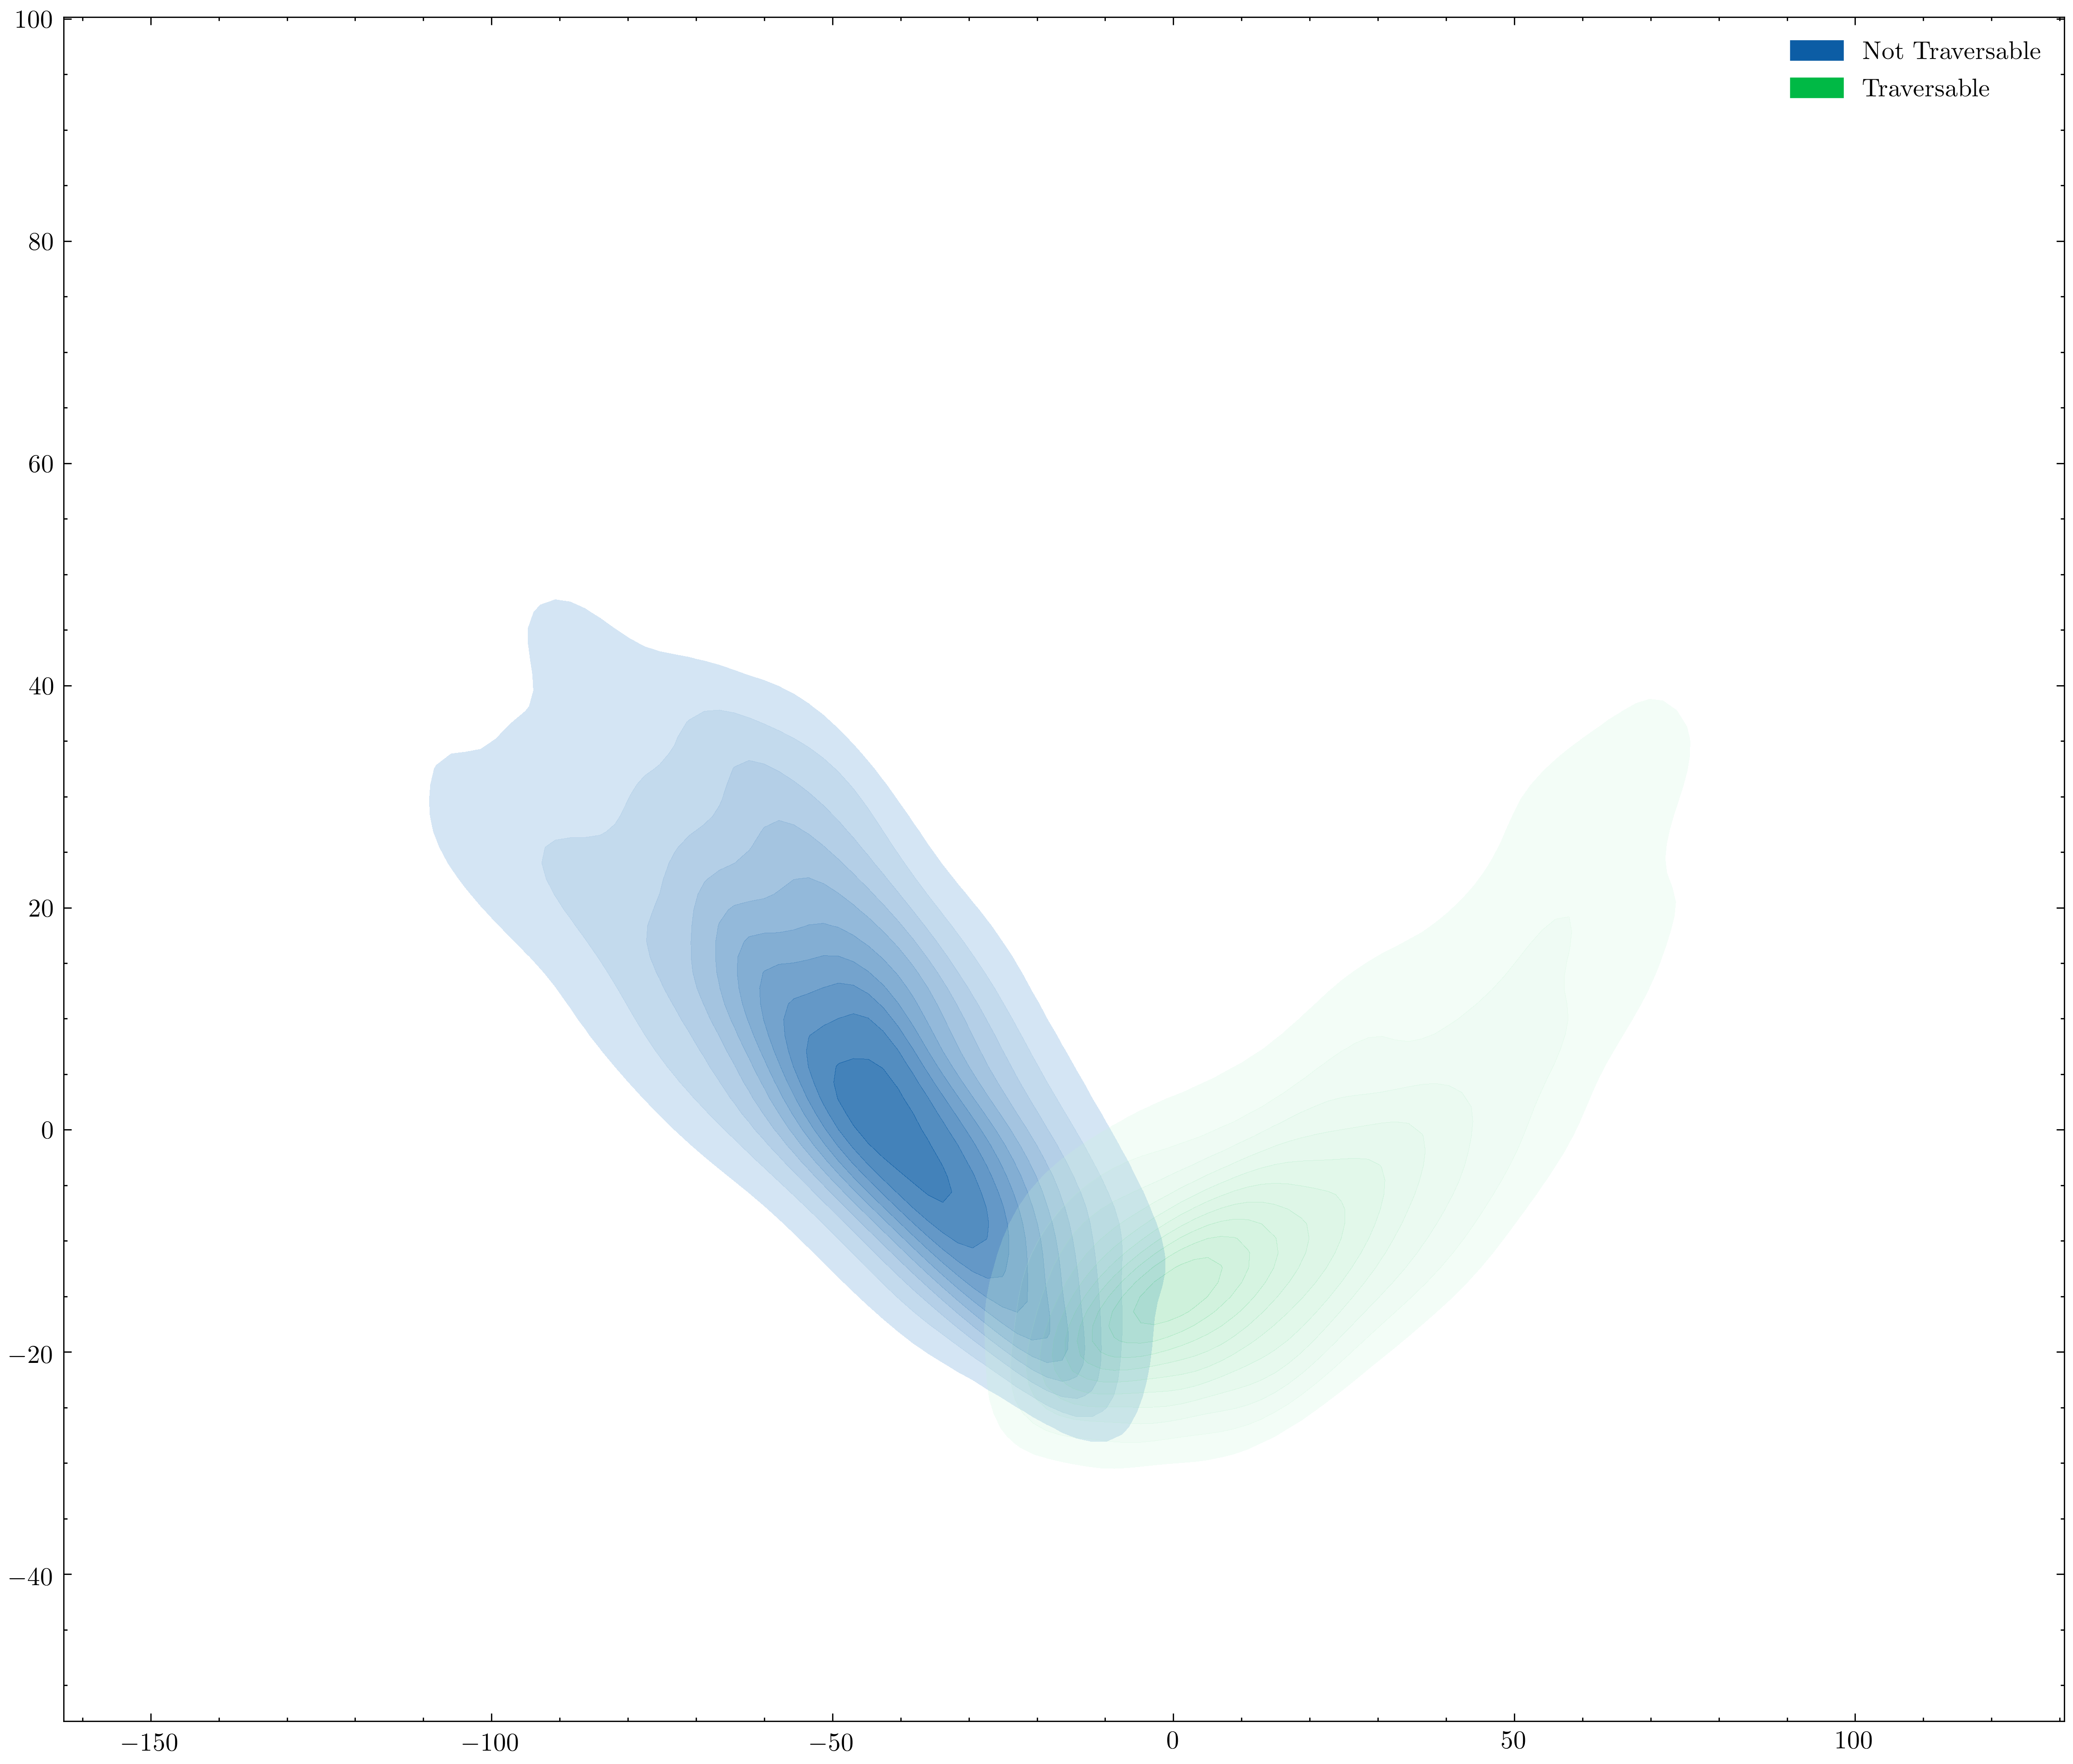
\includegraphics[width=\linewidth]{../img/5/pca/pca-0-density.png}
        \caption{Not Traversable}
    \end{subfigure}
    \begin{subfigure}[b]{0.48\textwidth}
        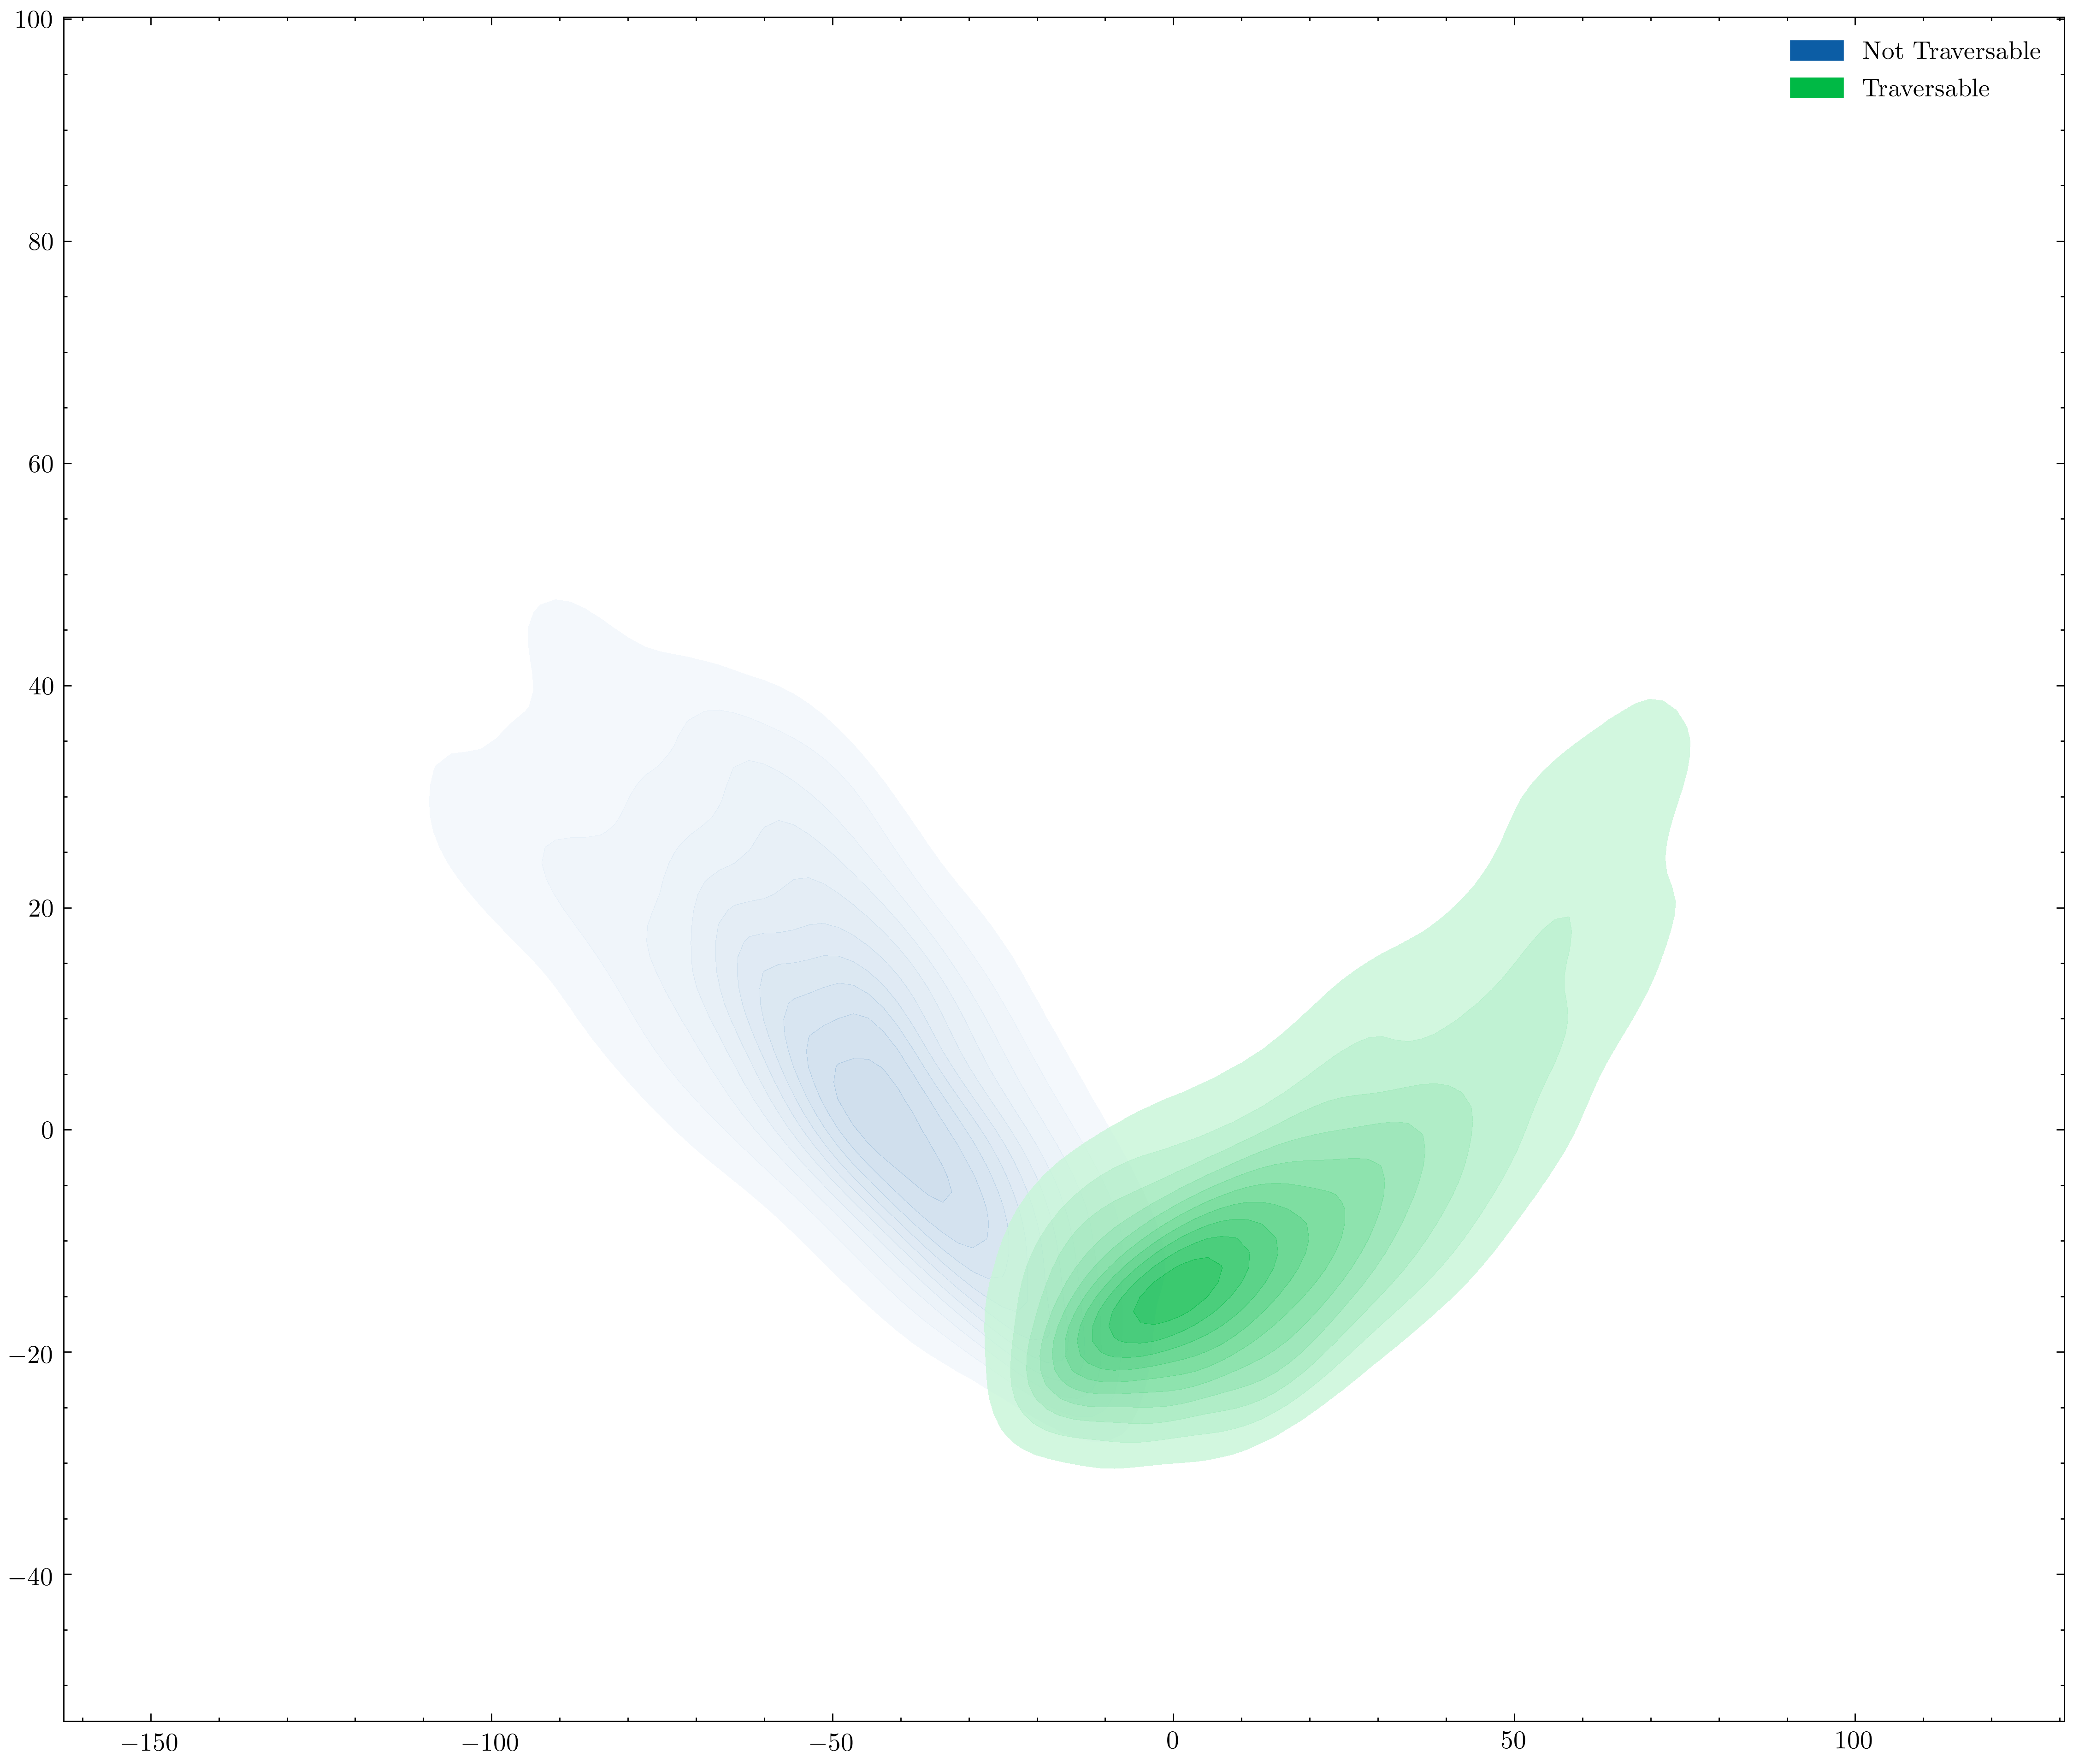
\includegraphics[width=\linewidth]{../img/5/pca/pca-1-density.png}
        \caption{Traversable}
    \end{subfigure}
    \caption{Density plot of the points sampled from the training dataset in the features space. The more opaque the color the close to the cluster center. The centers of the cluster are not overlapping yielding a good separability and correct learning.}
    \end{figure}
Clearly, there is some distance between the centers. Furthermore, we can directly plot the patch corresponding to each feature vector to identify clusters of patches based on their position. Intuitively, if similar inputs are close to each other in the features space then the model also learned to effectively encode terrains features. We decided to not show all images on the same plot to avoid overcrowding the image. Instead, we clustered the points using K-Means with $k=50$ clusters and then we took the patch that corresponded to the center point in each cluster. In this way, even by showing only a few inputs, we included all the meaningful ground types. Figures \ref{fig : pca-patches-200} visualizes the results.
\begin{figure} [htbp]
    \centering
    \begin{subfigure}[b]{1\textwidth}
        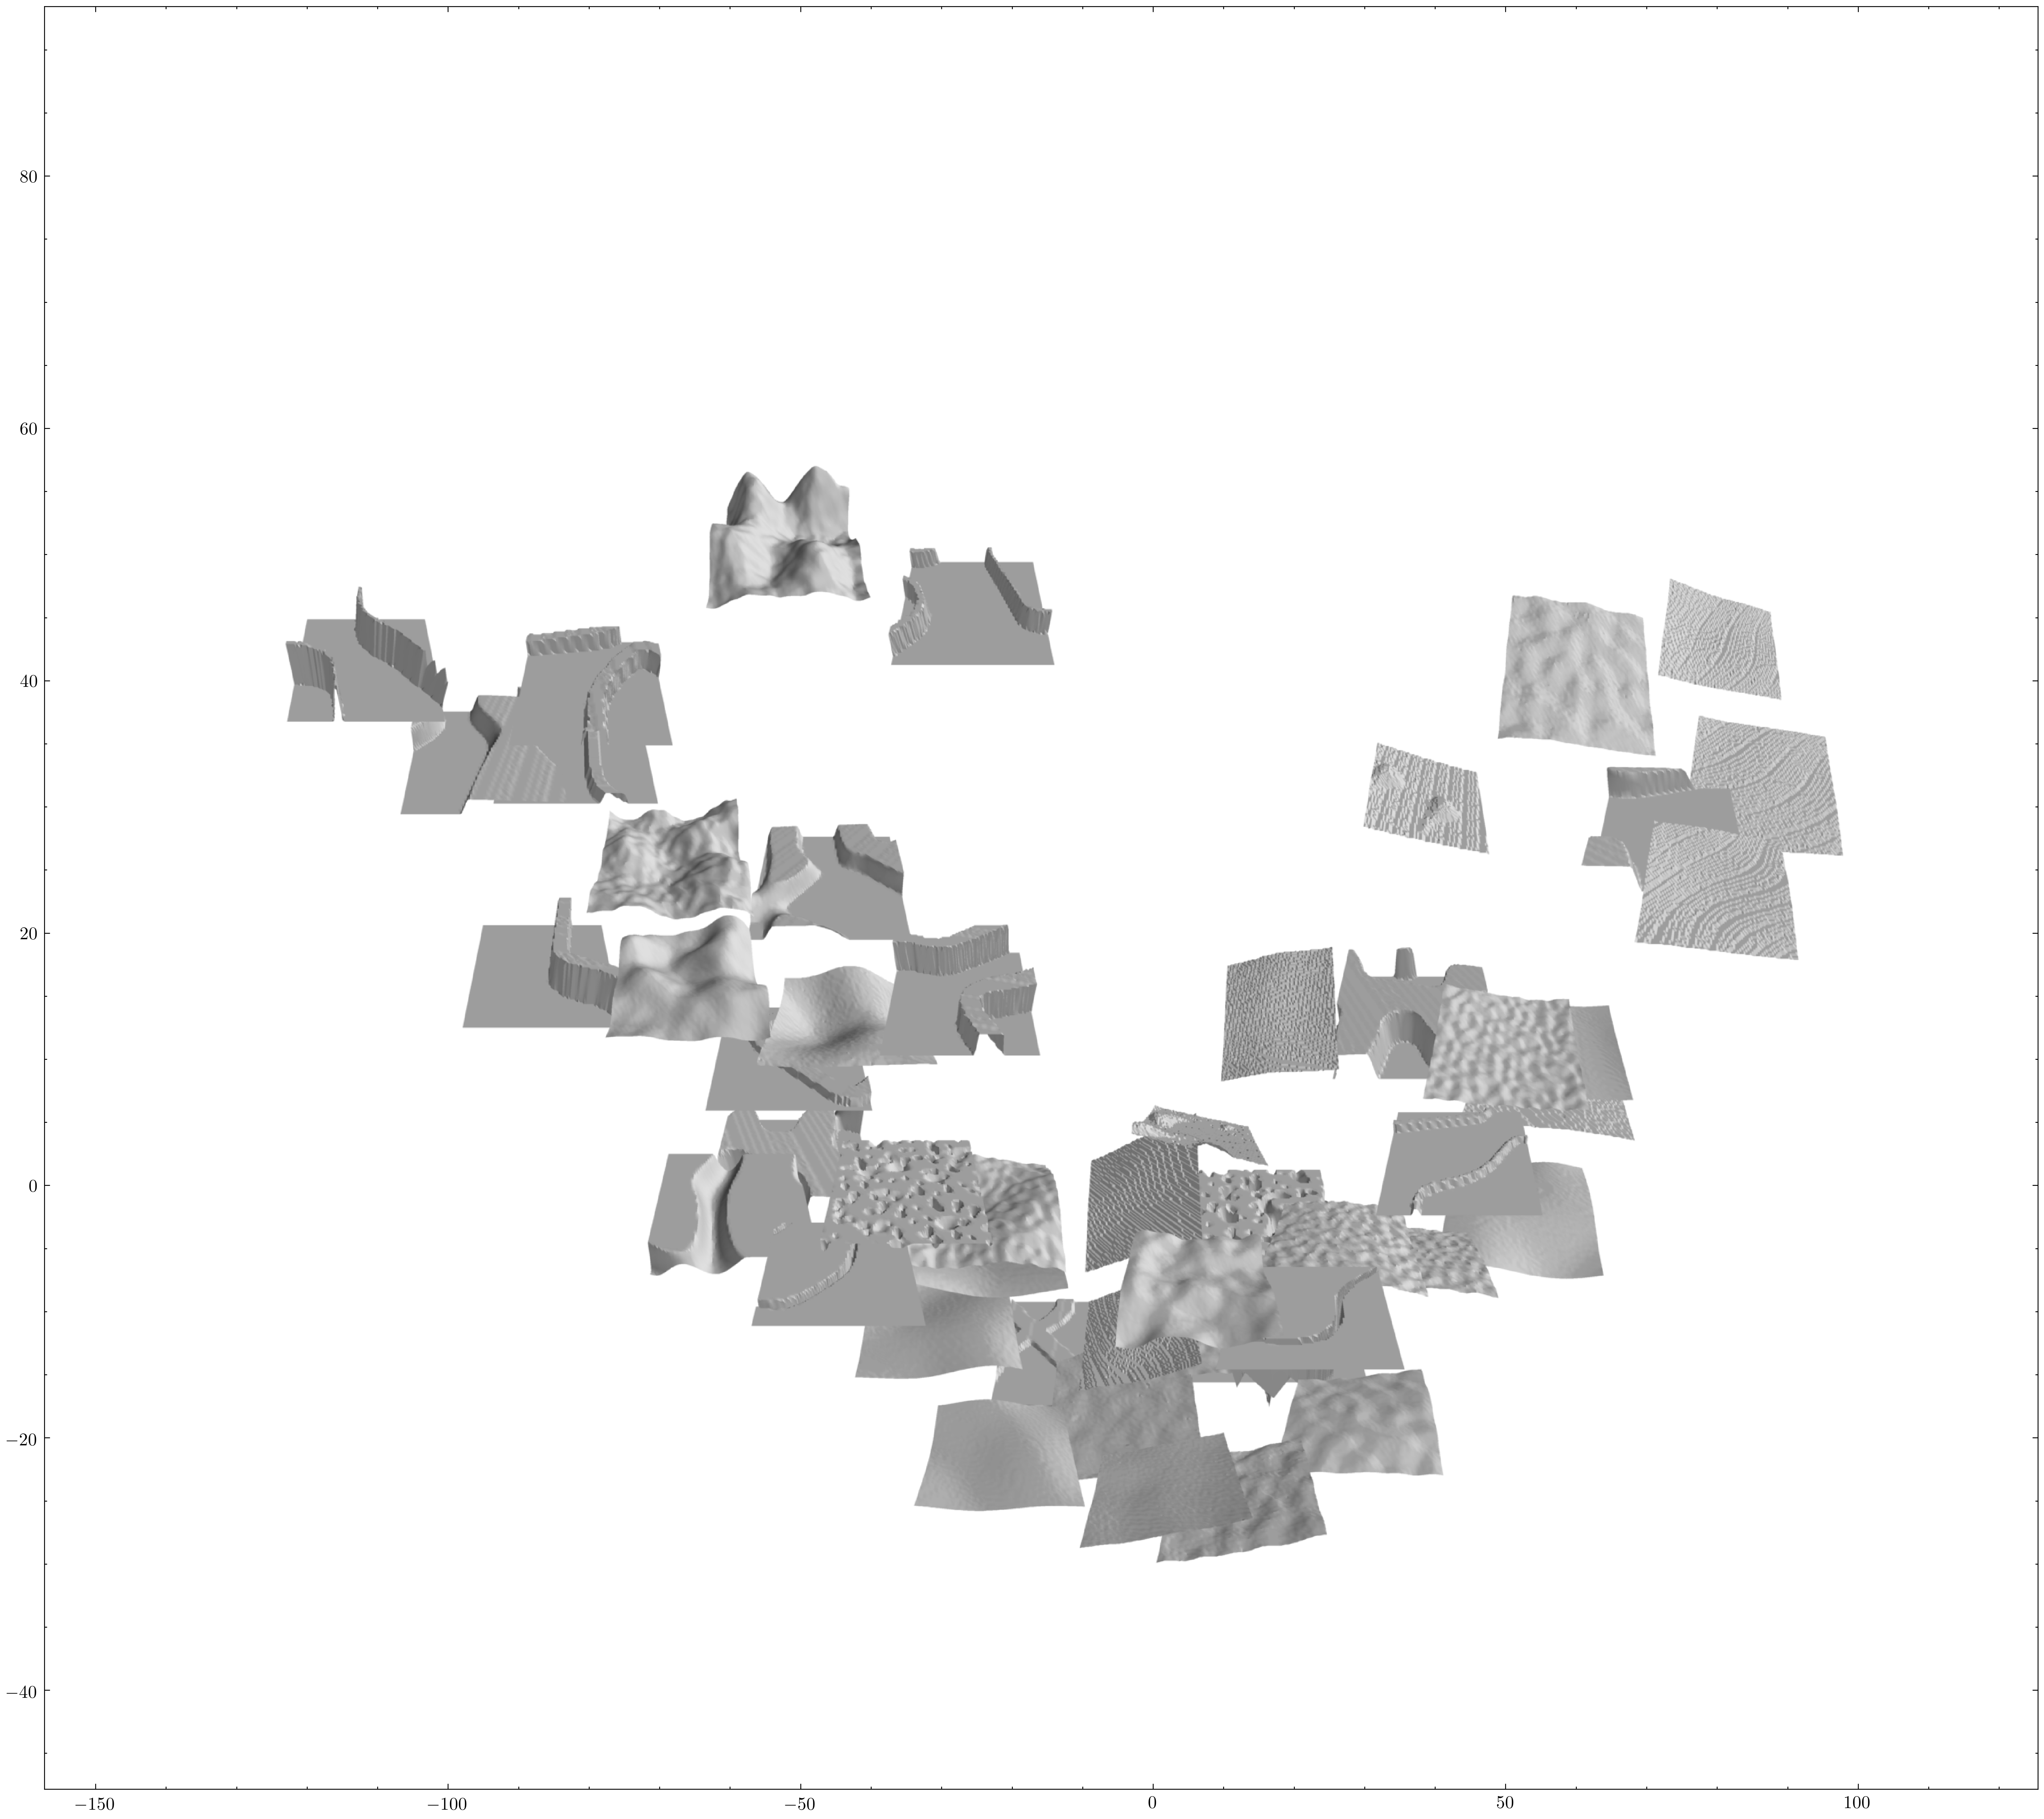
\includegraphics[width=\linewidth]{../img/5/pca/pca-patches-50-None.png}
    \end{subfigure}
    \caption{Patches plotted using the coordinate of the features vector obtained from the last convolutional layer's output and then reduced using PCA to a two-dimensional vector. Similar grounds are close to each other.}
    \label{fig : pca-patches-200}
\end{figure}
Definitely, patches with similar features are close to each other yielding a quality features encoding. On the left-top side, we can distinguish highly untraversable patches with walls/bumps in front of the robot. Going down, we encounter patches with smaller obstacles. On the plateau, there are traversable patches with small obstacles such as light bumps. Importantly,  those patches are the closest ones to the not traversable ones, so they were the hardest to separate, thus, to classify.  Going up on the right side, we see some grounds with small steps. Finally, on the top, we find all the downhill patches, the simplest ones to traverse.

\subsection{Features space of the test set}
We can apply the same procedure on the test set. Since it is a real world quarry, this dataset is harder than the train set and present challenging situations for the robot. The following image shows the features space after reducing its dimension to two using PCA.
\begin{figure} [htbp]
    \centering
    \begin{subfigure}[b]{1\textwidth}
        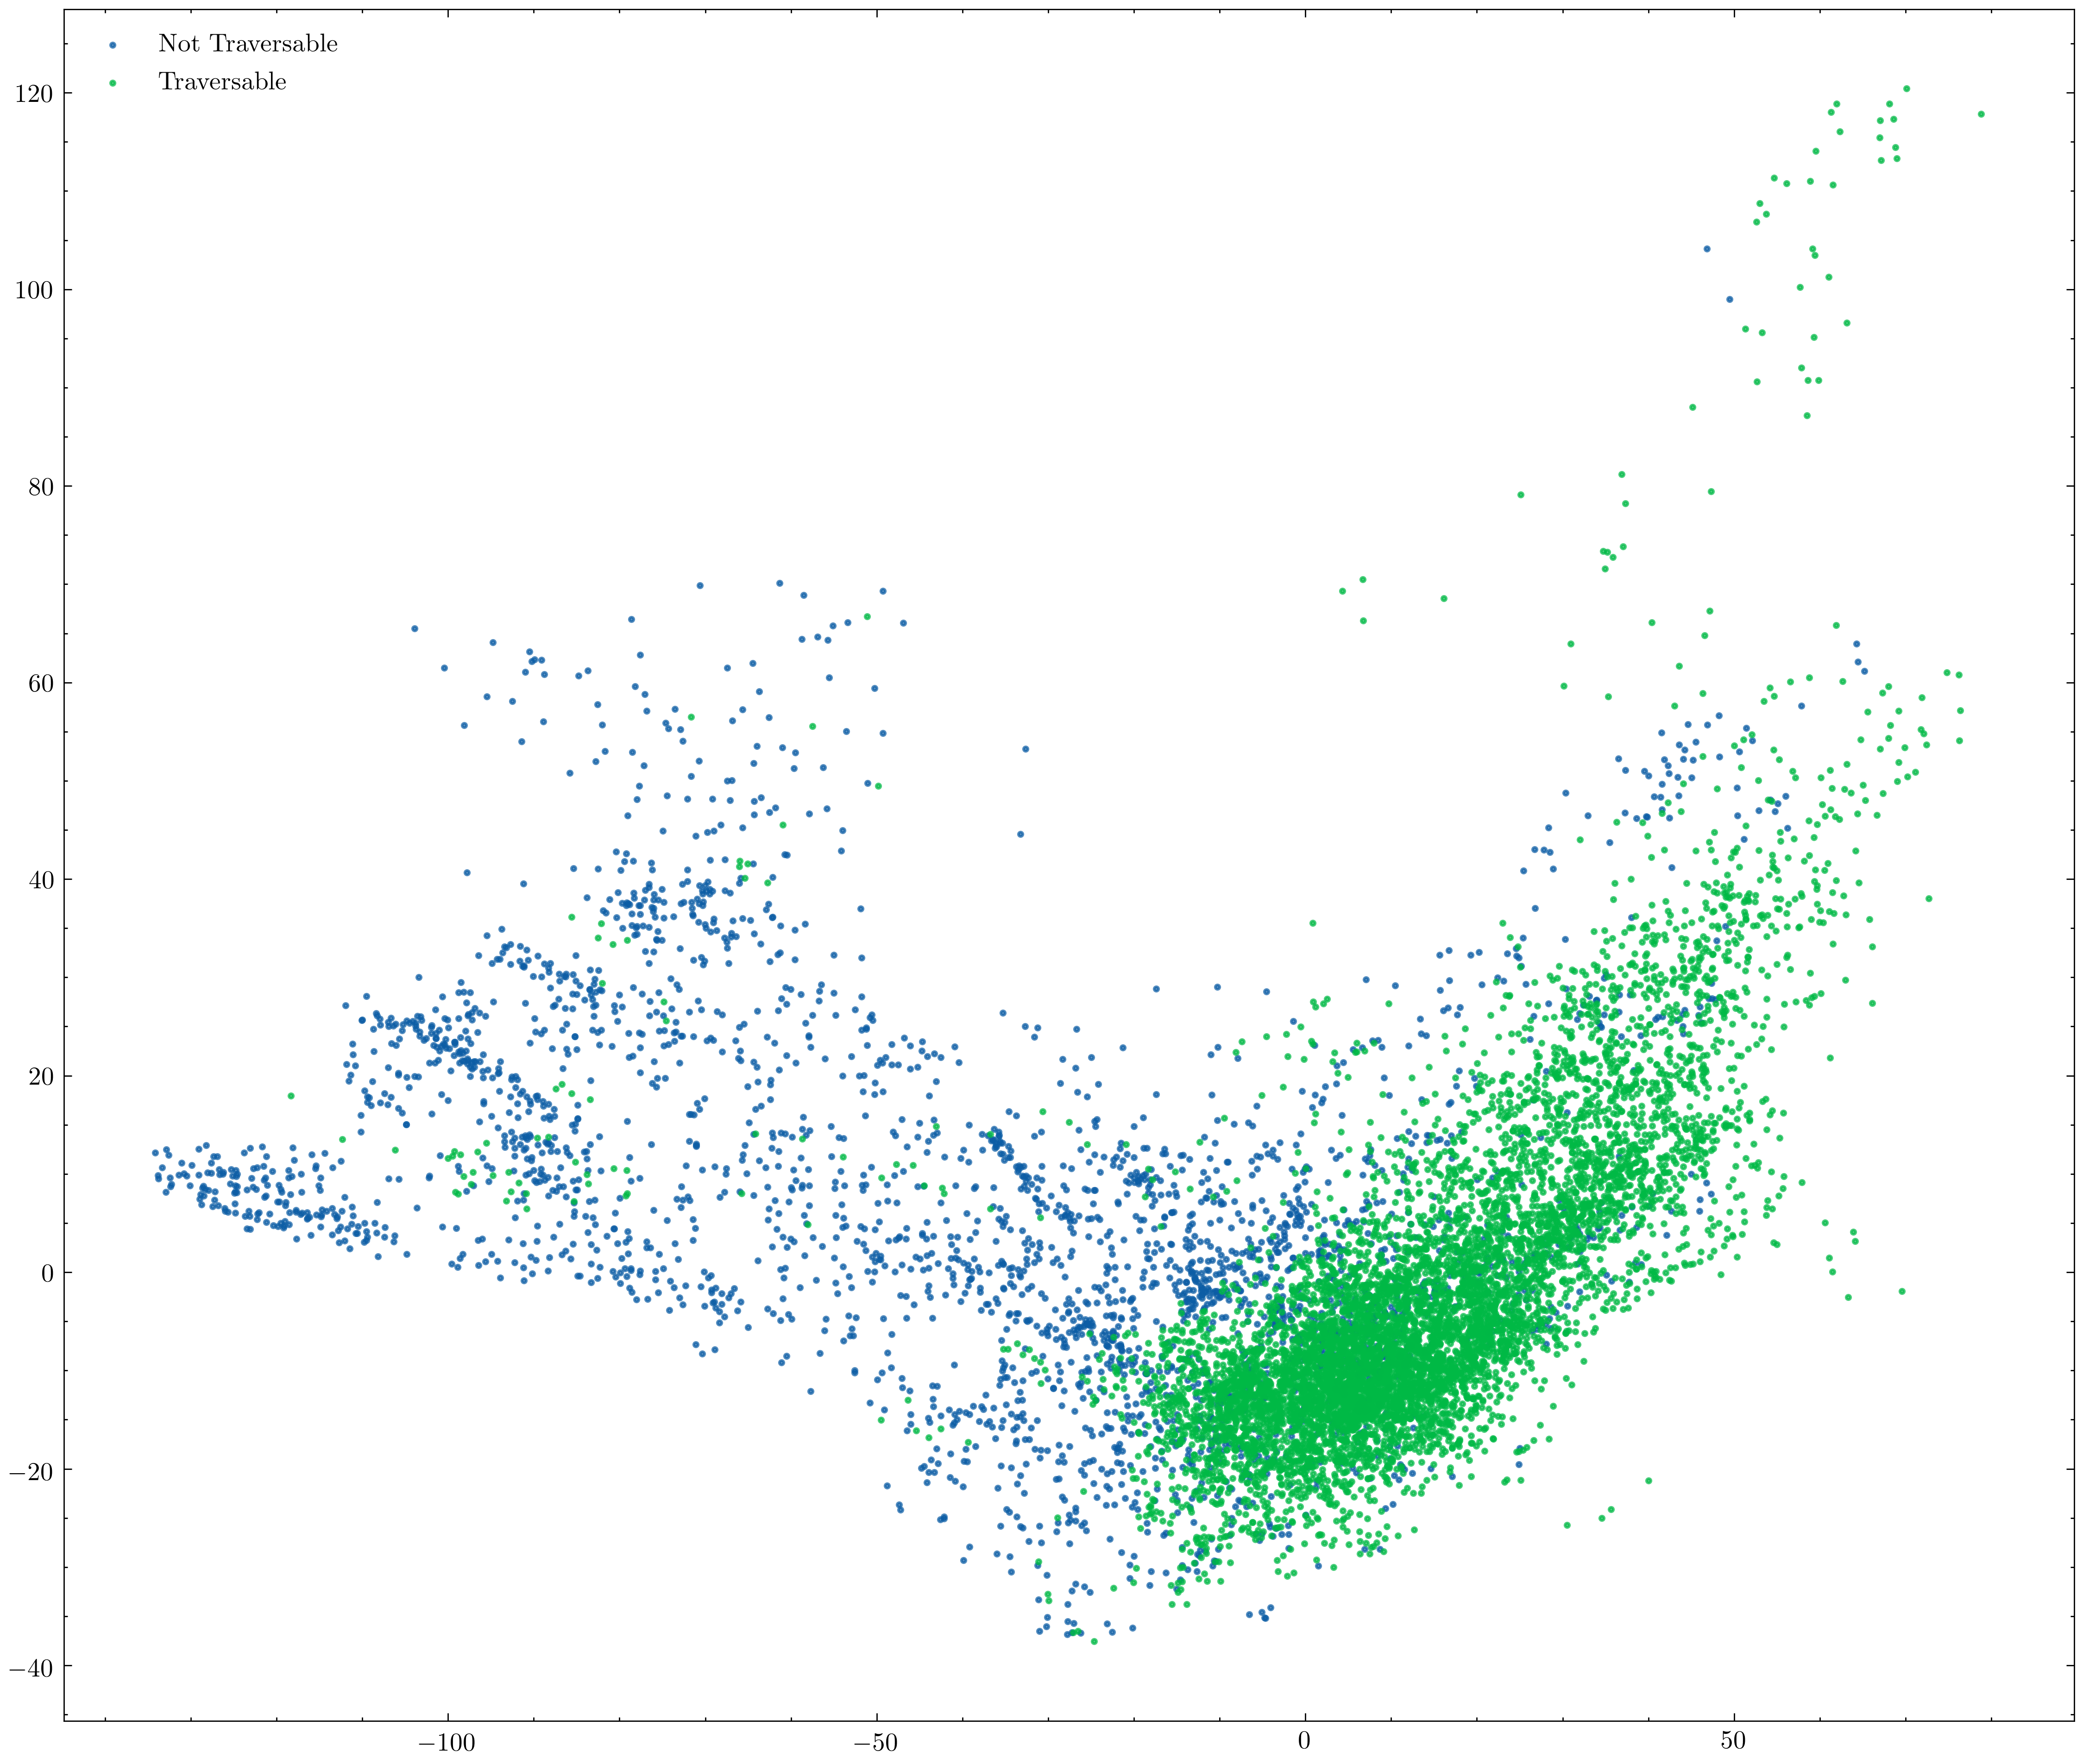
\includegraphics[width=\linewidth]{../img/5/pca/pca-test.png}
    \end{subfigure}
    \begin{subfigure}[b]{0.48\textwidth}
        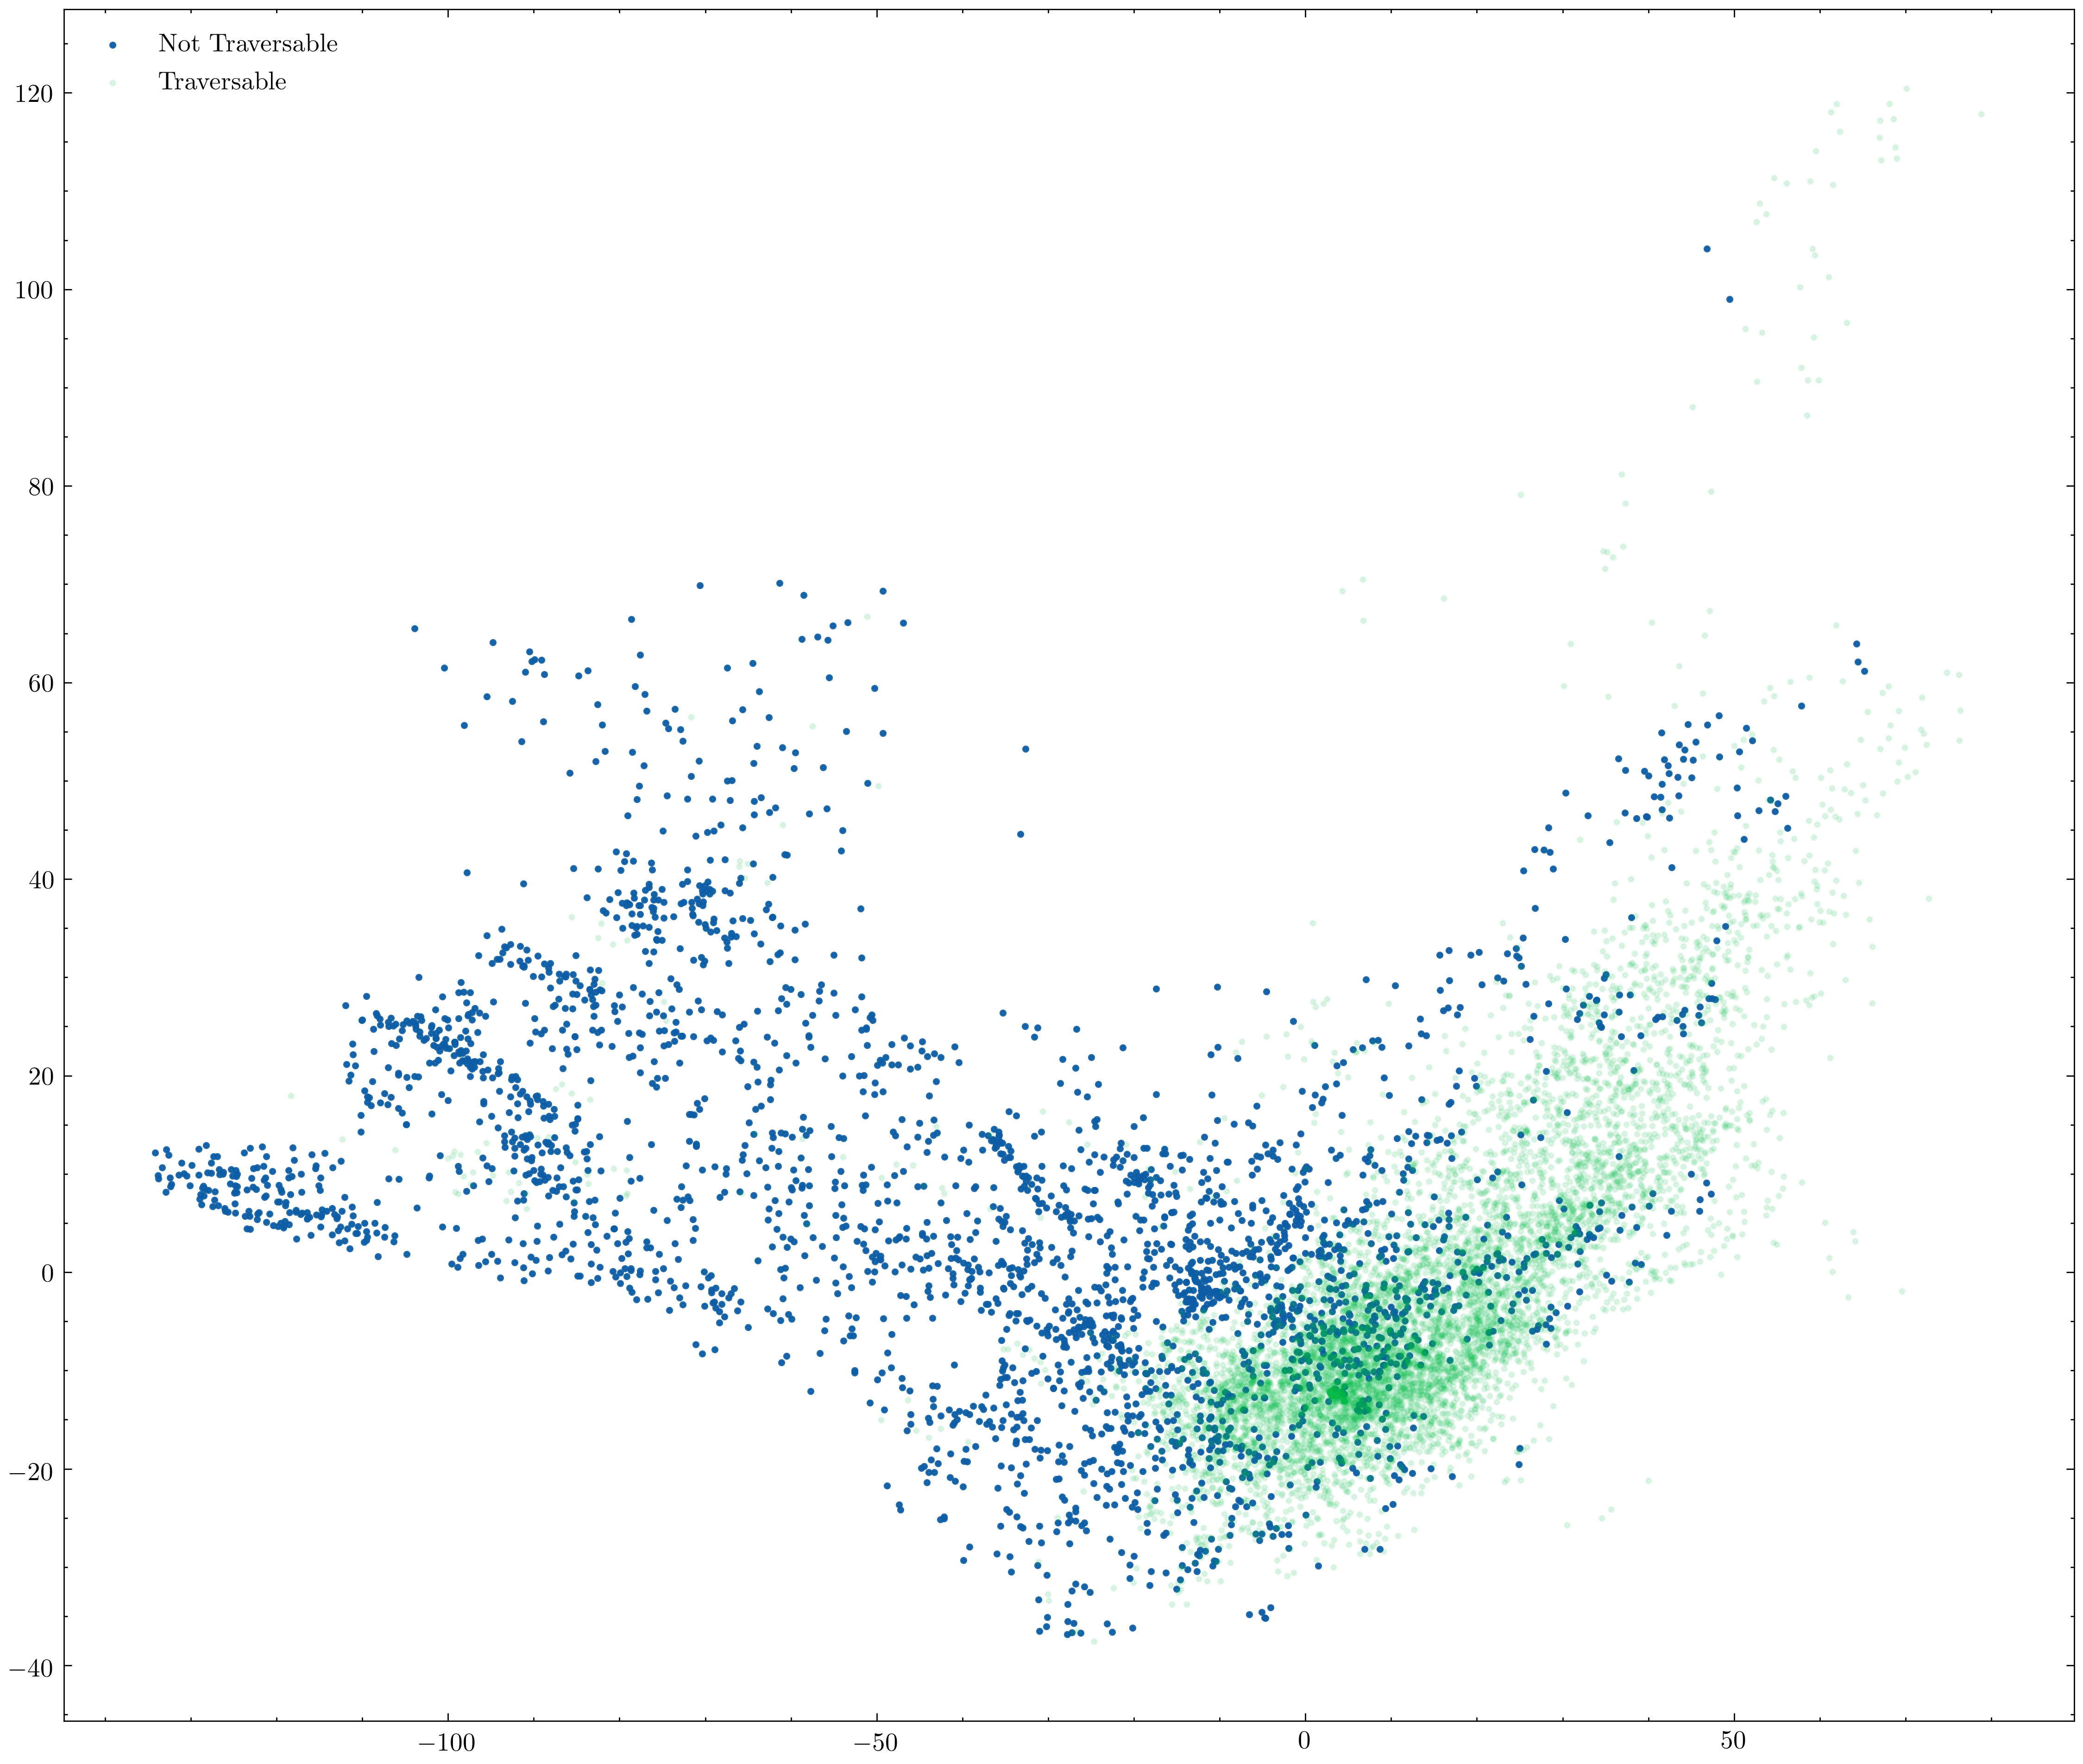
\includegraphics[width=\linewidth]{../img/5/pca/pca-test-0.png}
    \end{subfigure}
    \begin{subfigure}[b]{0.48\textwidth}
        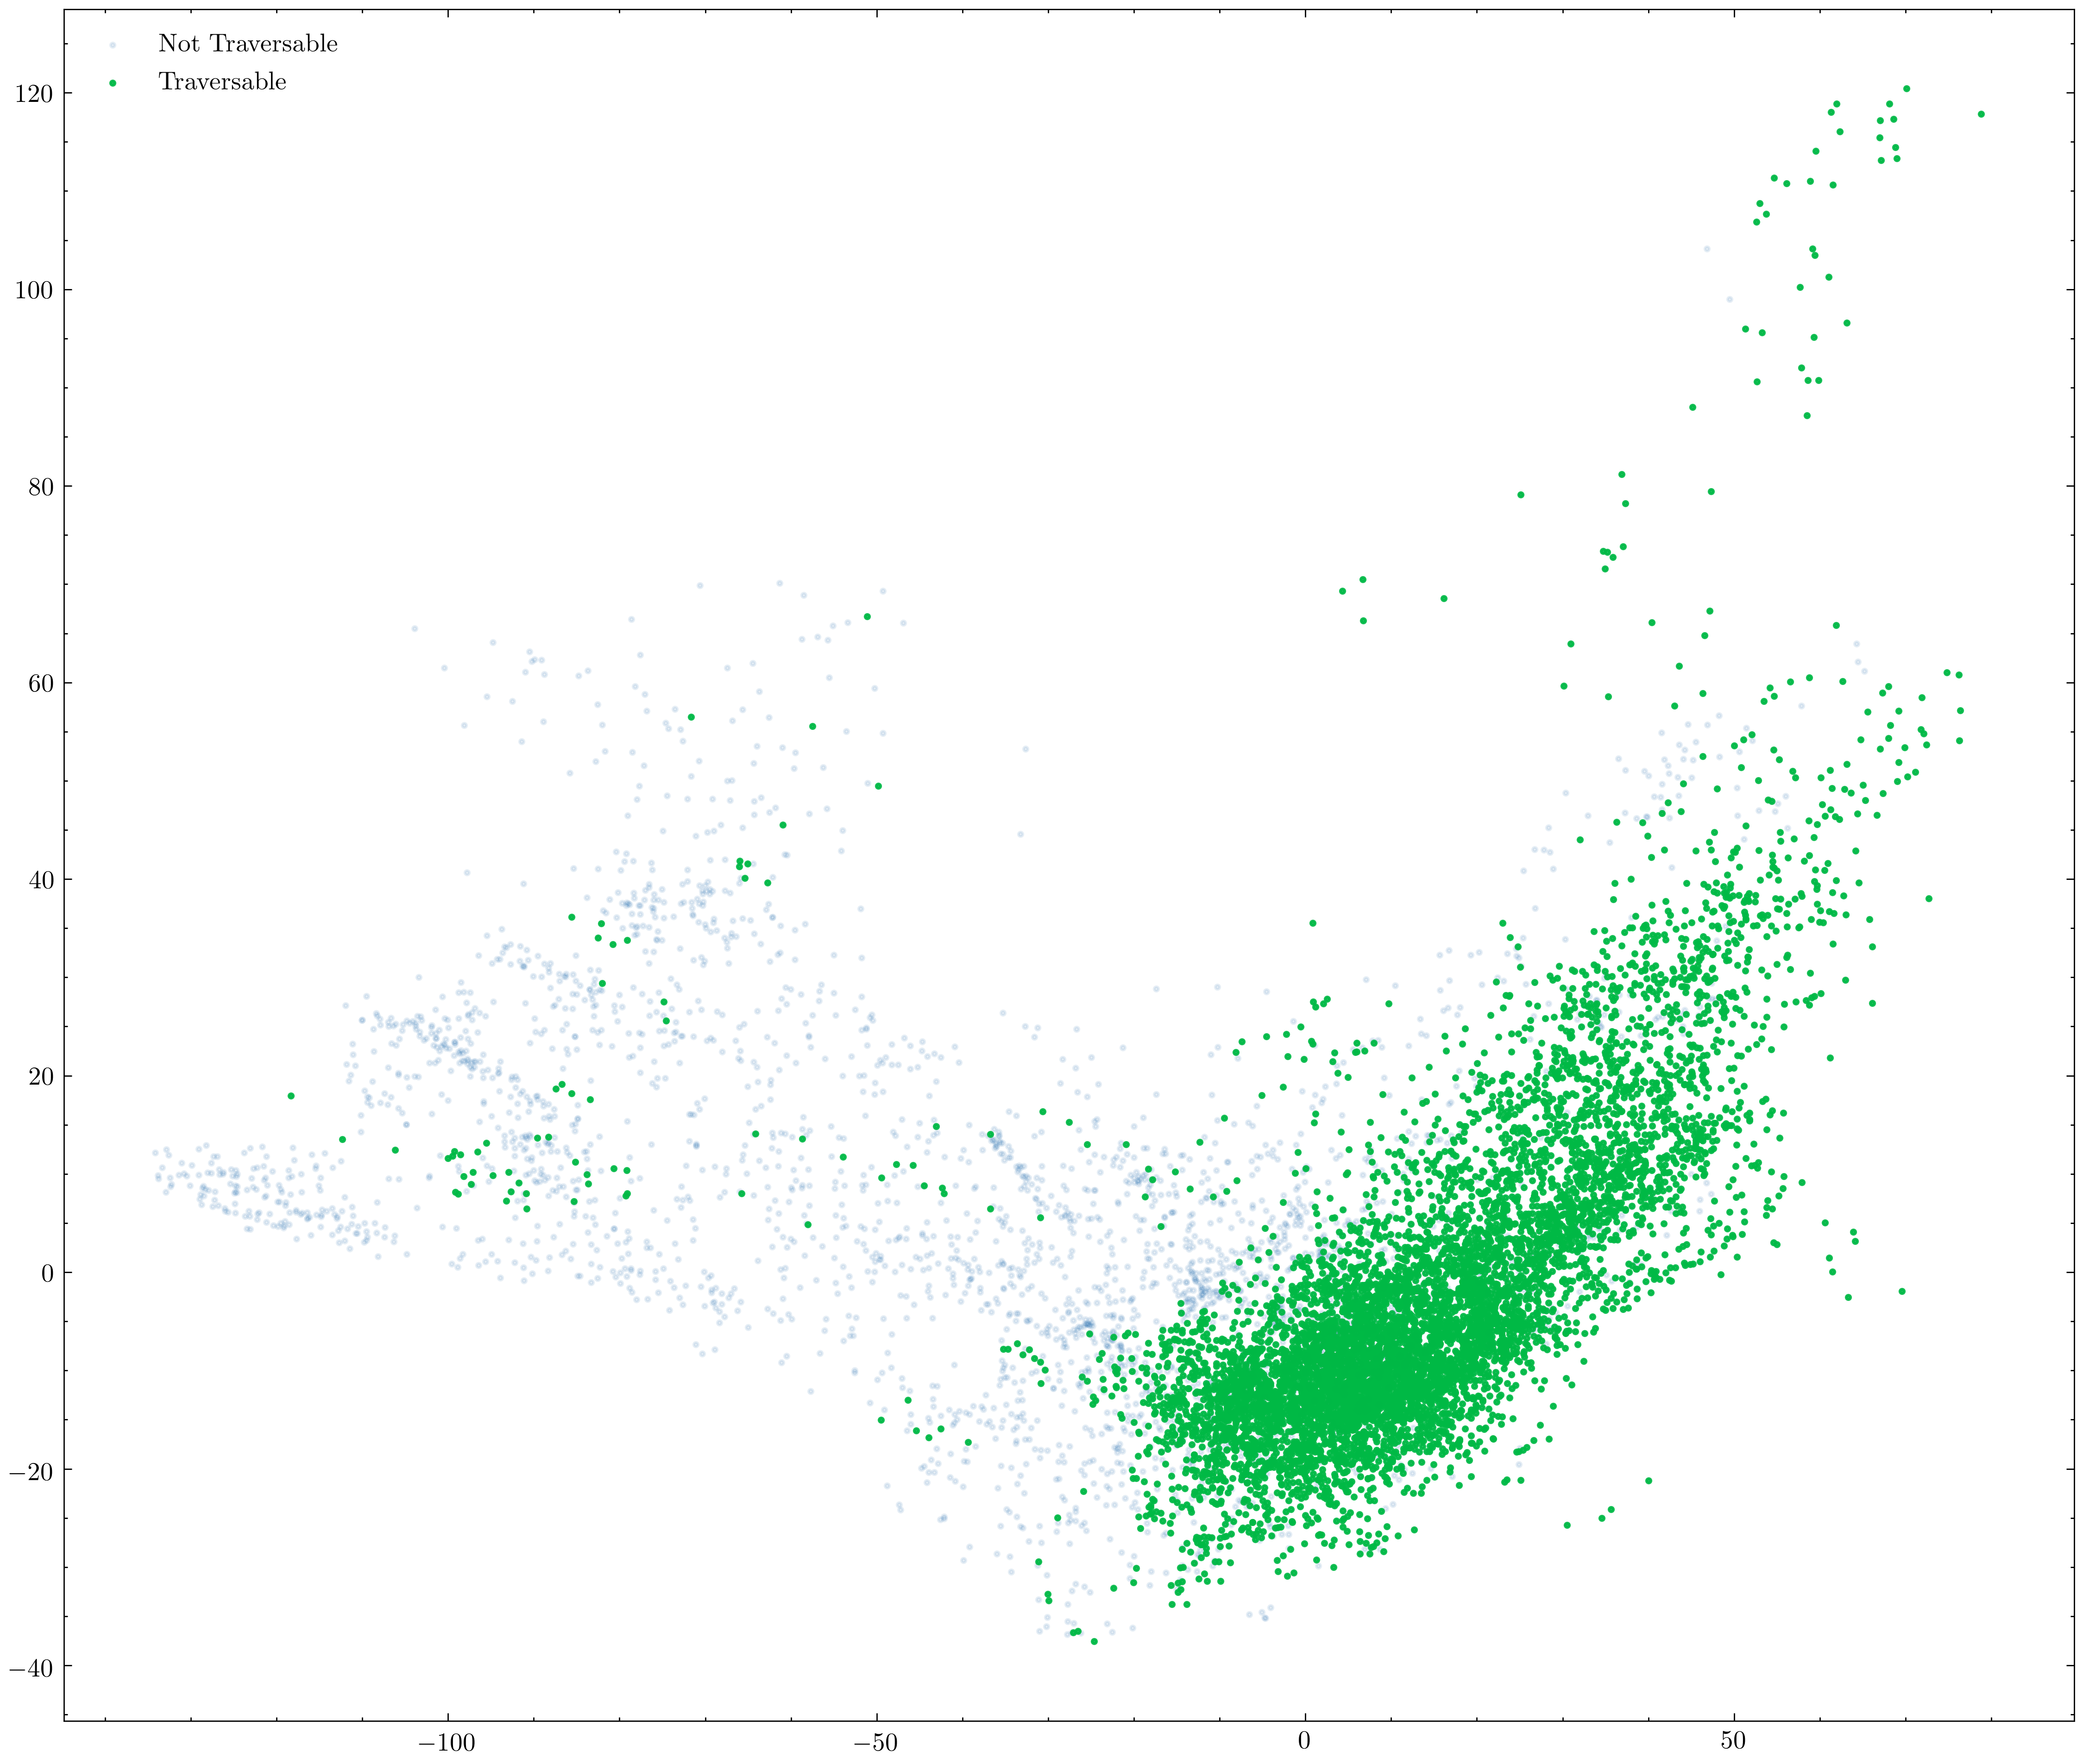
\includegraphics[width=\linewidth]{../img/5/pca/pca-test-1.png}
    \end{subfigure}
    \caption{Principal Component Analysis on the features space computed using the outputs from the last convolutional layers on the test dataset. We can distinguish two main clusters. However, some points are mixed up between classes.  }
    \label{fig : pca-test-set}
\end{figure}
Interesting, the traversable patches in figure \ref{fig : pca-test-se} are very near to each other, while the others span a very big surface. This suggests that there are many not traversable terrains with different features. The traversable points are clustered near the center, this implies that most of them share similar features. We plotted the density for each class to better understand where the most points are mapped.
\begin{figure} [htbp]
\begin{subfigure}[b]{0.48\textwidth}
    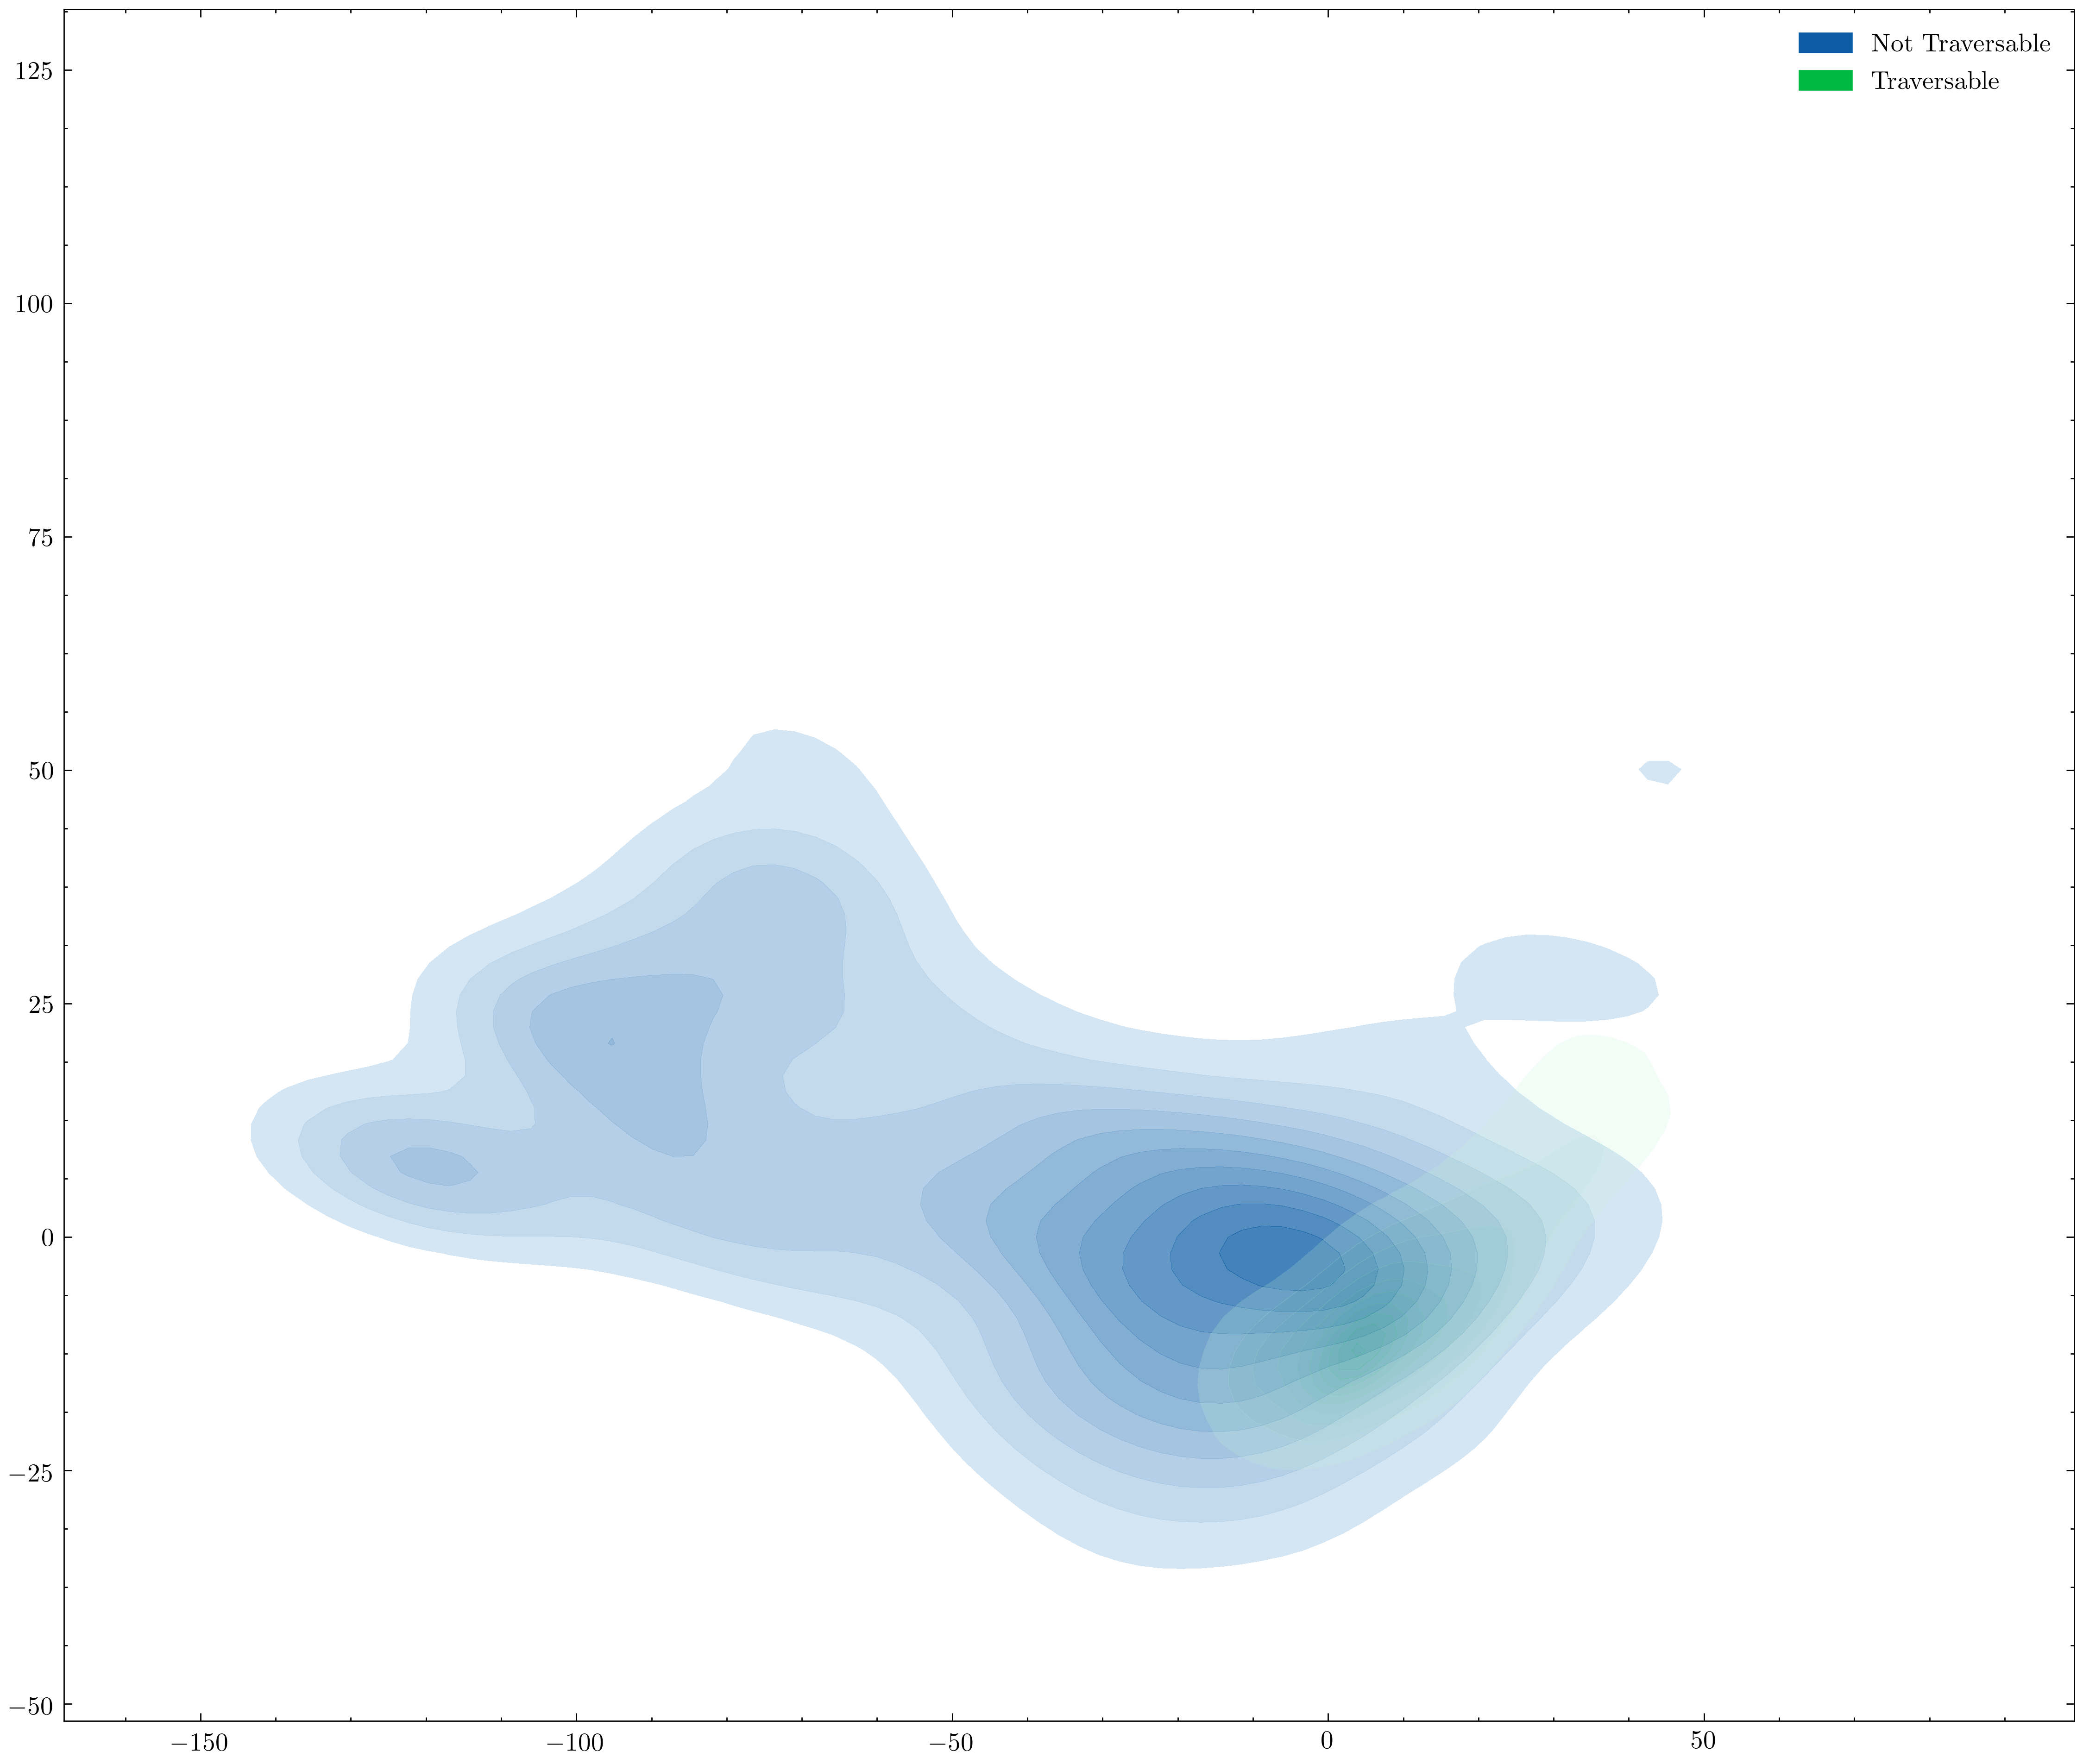
\includegraphics[width=\linewidth]{../img/5/pca/pca-test-0-density.png}
    \caption{Not Traversable}
\end{subfigure}
\begin{subfigure}[b]{0.48\textwidth}
    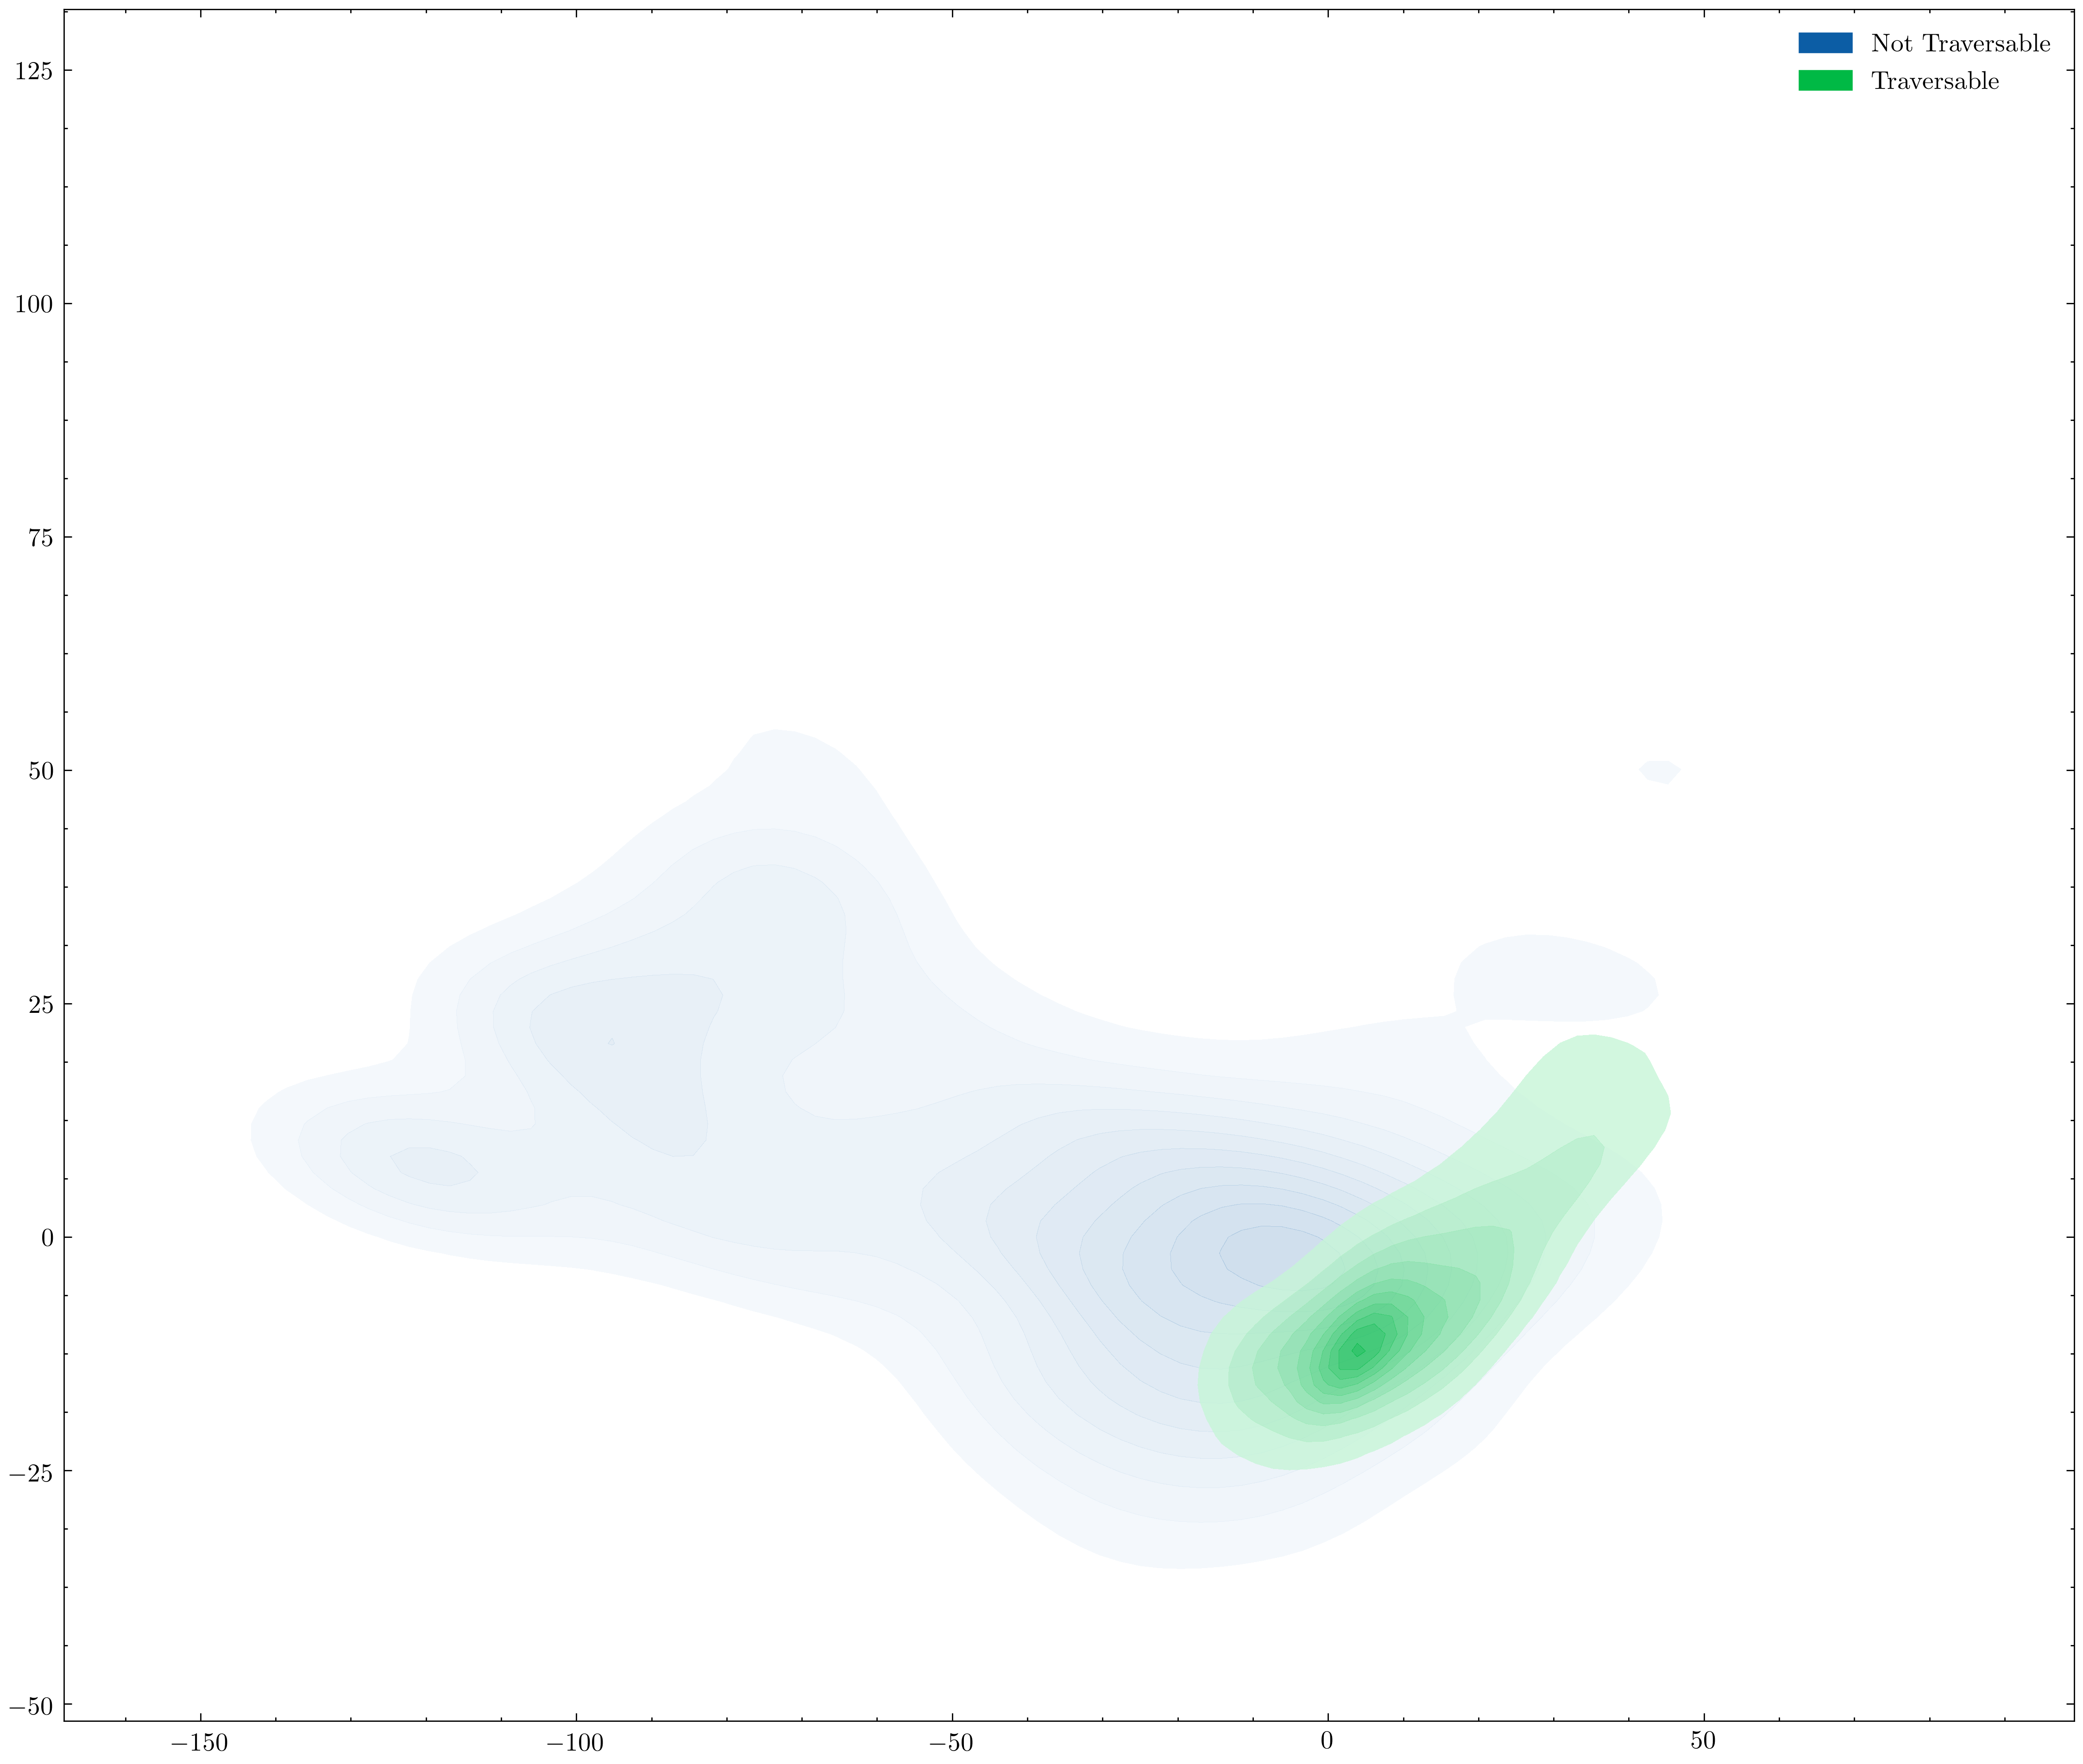
\includegraphics[width=\linewidth]{../img/5/pca/pca-test-1-density.png}
    \caption{Traversable}
    \label{fig : pca-test-density-1}
\end{subfigure}
\caption{Density plot fofor the points sampled from the test dataset in the features space.  The more opaque the color the close to the cluster center. The centers of the clusters are close to each other yielding less separability/}
\end{figure}
The two centers are really close to each other, making those samples harder to separate and some not traversable points are mixed up with the traversable ones. This explains the elevated number of false negative that lower down the AUC score on this dataset. We can also visualize the patches by plotting them using their features coordinates
\begin{figure} [htbp]
    \centering
    \begin{subfigure}[b]{1\textwidth}
        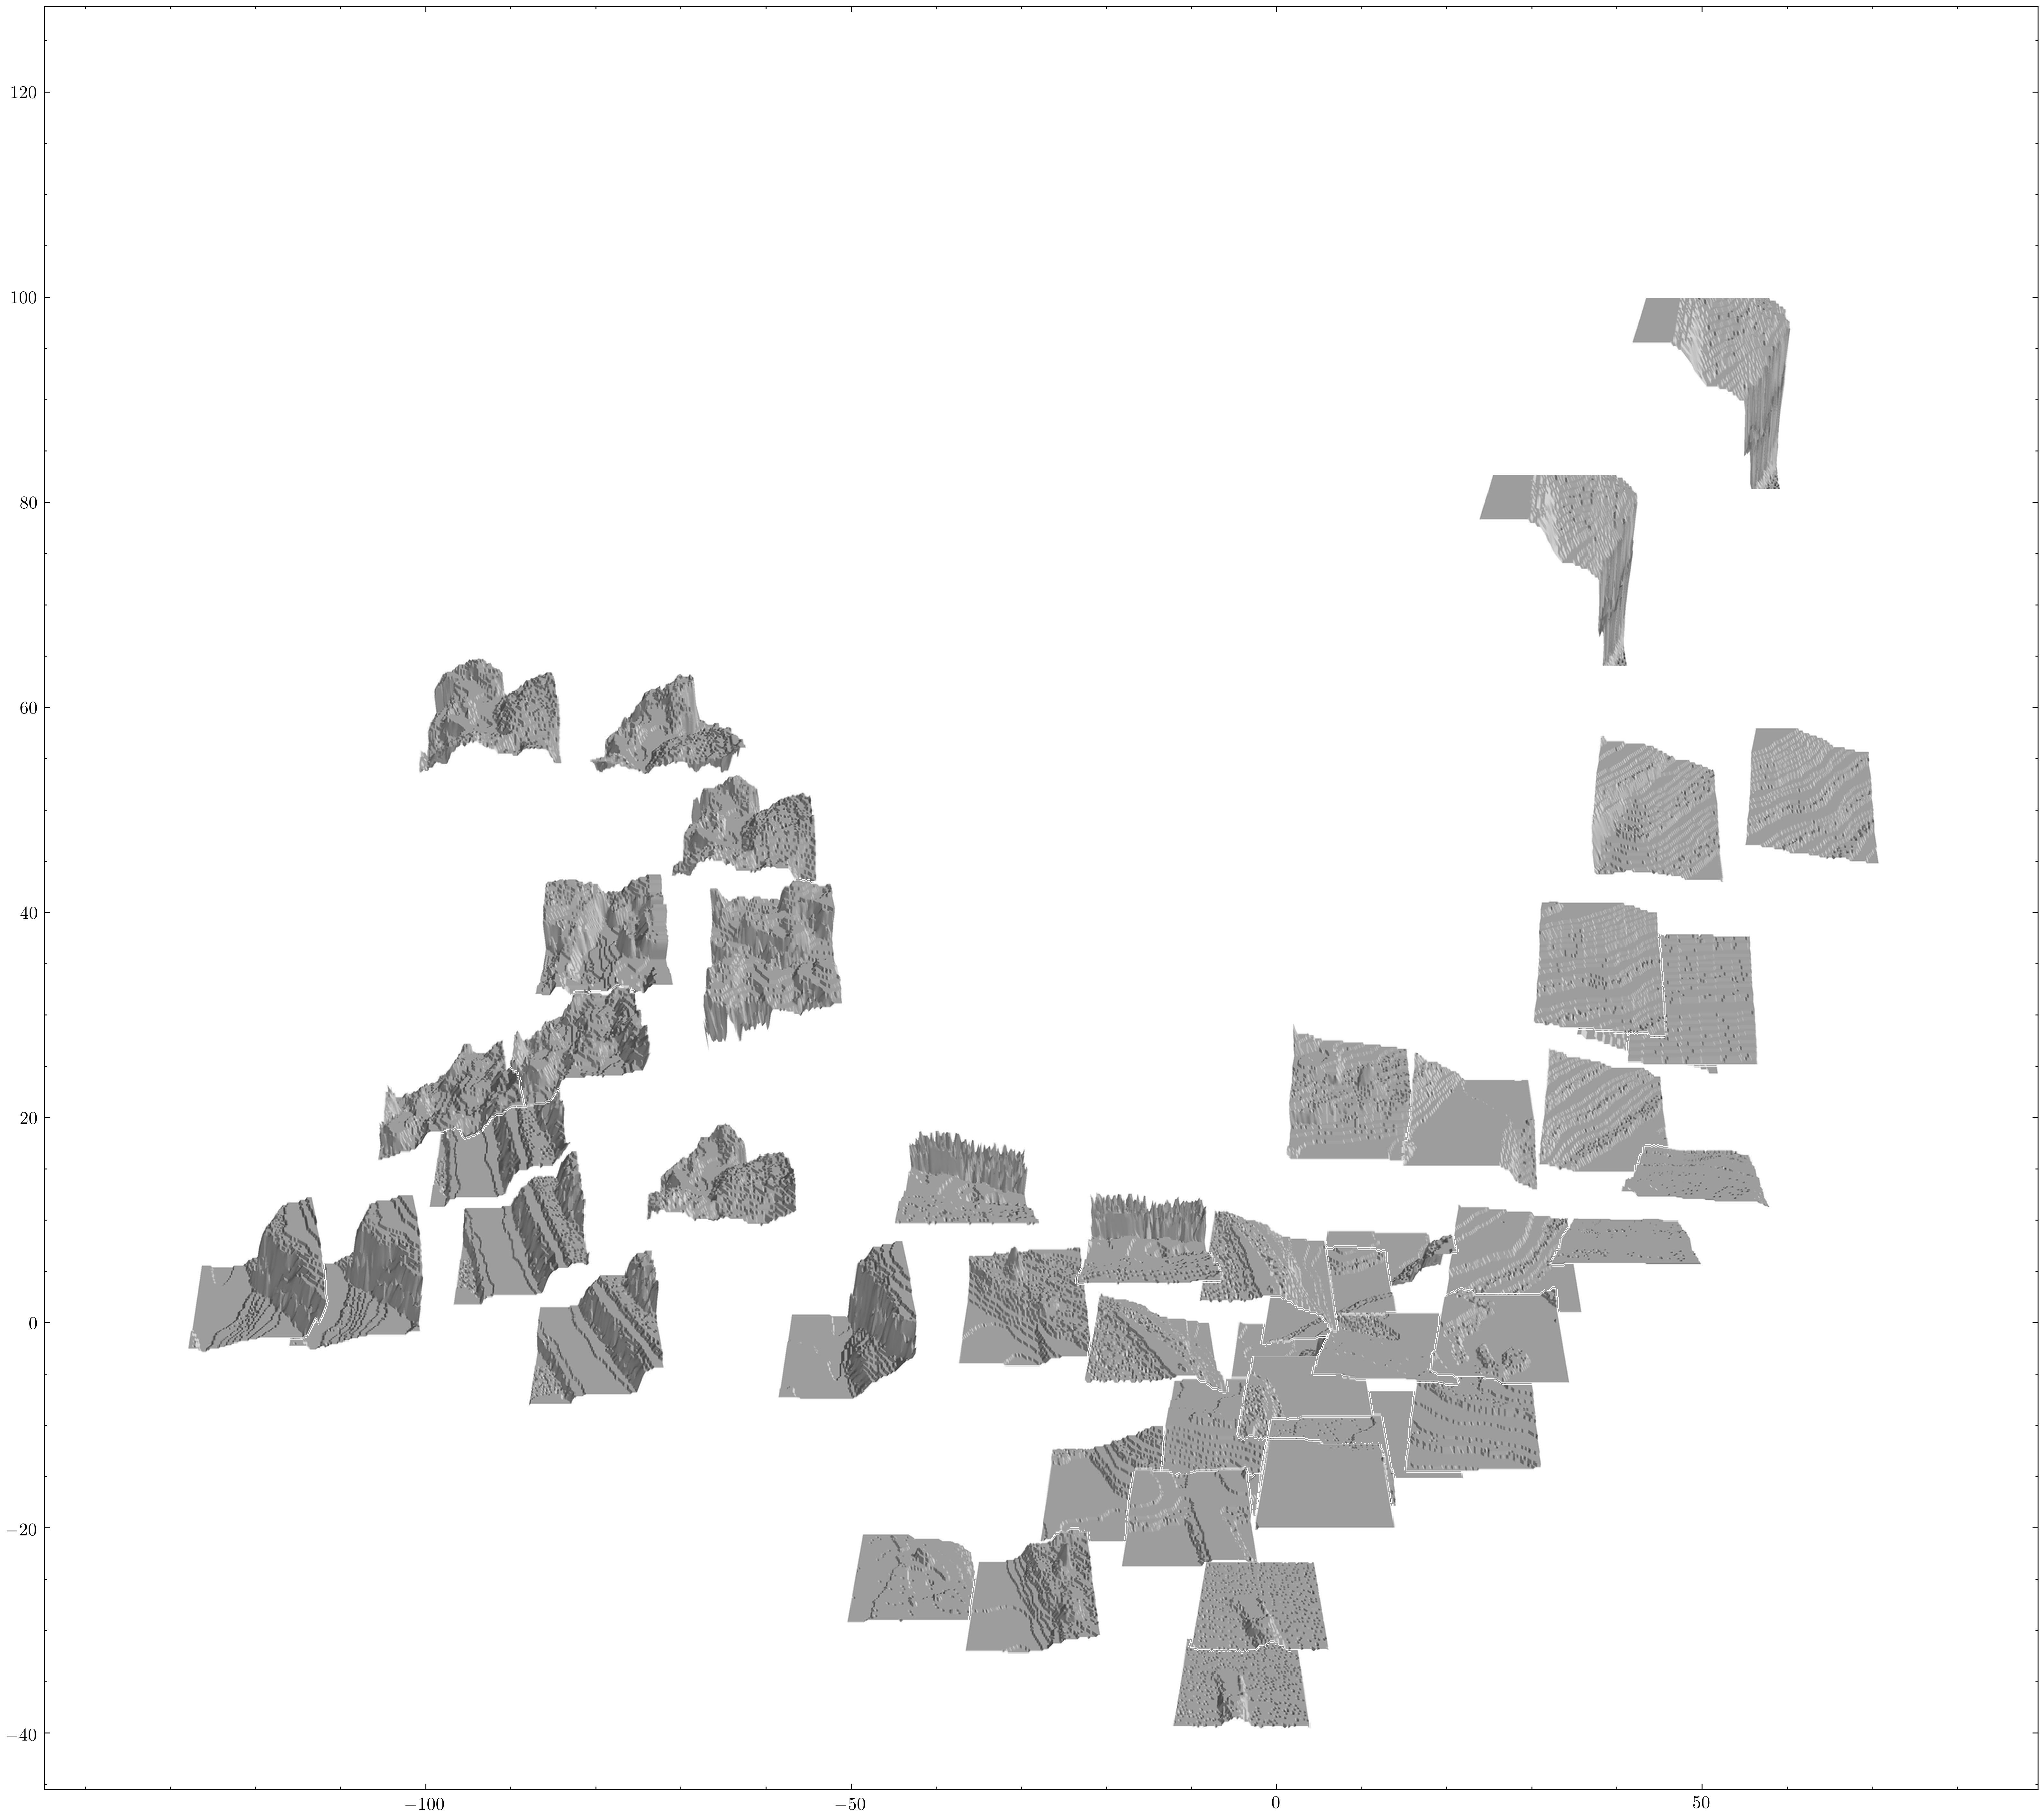
\includegraphics[width=\linewidth]{../img/5/pca/pca-test-patches-50-None.png}
    \end{subfigure}
\caption{Patches that correspond to coordinates in the features space of the last convolutional layers on the test dataset. Similar grounds are close to each other.}
\ref{fig: pca-test-patches}
\end{figure}
On the top left, from the not traversable cloud, we can see patches with a high level of bumps. Going down we find surfaces with huge walls in front of the robot while going close to the center we start to see all the traversable patches. Those samples have not too steep slopes. If we move to the density center, green double shown in figure \ref{pca-test-density-1}, we encounter lots of flat patches with little obstacles. Going up on the right branch we find downhill and on the top there are falls. 

In the following section, we will take a deep look at the test set to find which patches confuse the most the model. Probably, those samples will be located between the two clusters' center where the difference between classes' features is minimum. 

\documentclass[../document.tex]{subfiles}
\begin{document}
\section{Quarry dataset}
\label{sec: quarry-dataset}
After showing the model's capability of correctly separate classes' features we utilized Grad-CAM to visualize some of the samples in the test set. The aim of this section is to show how the model looks at meaningfull features in each inputs to make the prediction even if its prediciton is wrong. For instance, imagine we feed to the model a not traversable patch with an obstacle and the network label is as traversable. Obsliously, the output is wrong but two situation may happened that effect the degree of 'wrongness'. First, the model could just have ignored the obstcle and looked away, meaning if was not even able to understand it should have loook there. Second, the network could have correctly look at the obstacle but thouhgt that maybe the obstacle was not tall enough, showing a correct ability to find and use important features in the map. We showned that, even when the predictions are wrong, our model always look at the most important features of each input to determine its traversability. 

We divided those inputs in four classes based on the model's performance: worst, best, false positive and folse negative. Then, we took twenty inputs from those sets and appplied Grad-CAM as texture on the 3D render to better visualize which region of the inputs caused the prediction. 
% \subsection{Best}
% We start evaluating our model by using the test set composed by samples from the Quarry map. We expect the model to correctly classify the patches with easy to see features such as big obstacles, steep ramps and holes. Unfortunately, the dataset is not trivial and most of the patches are challenging to classify even to human eye. 

% For instance, if look at patches, for some of them is not so easy to estimate the advancement by human eye. This is due to the specific robot locomotion that depends on the starting pose. Our goal in this section is to explain the model predictions on different inputs. 

\subsection{Best}
Best patches have few obstacles. We can obsverse two main clusters of images, flat and slopes. Interesting, when a surface has uneven ground near the left part, so close the the rear legs of the robot, the model is more interesting in those spots, \ref{fig : quarry-best-0}, \ref{fig : quarry-best-2}, \ref{fig : quarry-best-3}, \ref{fig : quarry-best-4}, \ref{fig : quarry-best-15}, \ref{fig : quarry-best-16}, \ref{fig : quarry-best-17}, \ref{fig : quarry-best-18}. This an expected behaviour since if there is an obstacle near the rear legs, then the robot will not be able to advance since it will be stuck from the beginning. 

Moreover, in other patches \ref{fig : quarry-best-1},  \ref{fig : quarry-best-8},  \ref{fig : quarry-best-9},  \ref{fig : quarry-best-19}, the model's also looks ahead of the robot. In those situation the robot is able to properly move at the beginning so the network must evaluate the possibility of obstacles ahead. There are two oblious cases, \ref{fig : quarry-best-8} and  \ref{fig : quarry-best-19}. The first one is a totally flat surface, so the model will look as far as possible to the robot's position to check if there are obstacles. Simarly, in the second, a surface with a bump in the hend, the network controls that spot. So, correctly, the network analysis the first region of the patch that may contain an untraversable obstacle.
\begin{figure}[H]
    \centering
    \begin{subfigure}[b]{0.192\linewidth}
    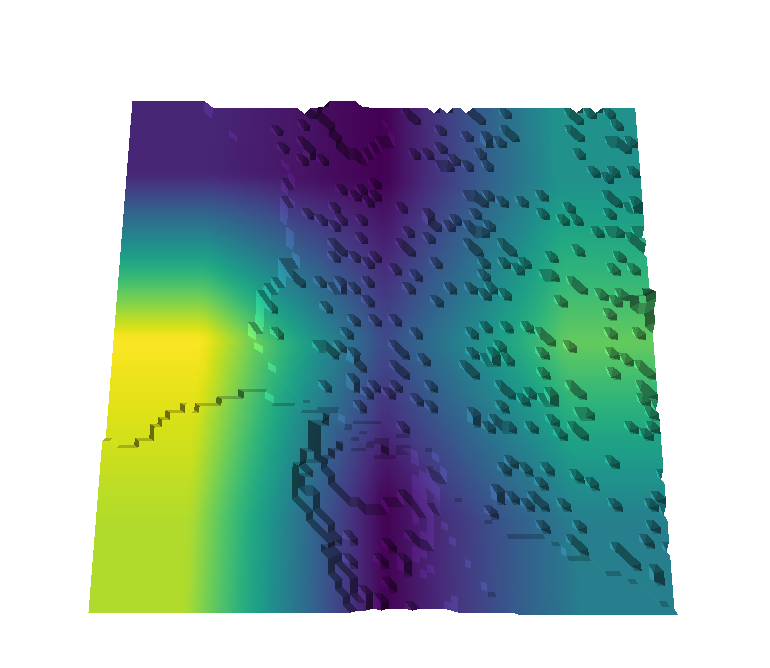
\includegraphics[width=\linewidth]{../img/5/quarry/best/20-patch-3d-majavi-colormap-0.png}
    \caption{0.20cm}
    \label{fig : quarry-best-0}
    \end{subfigure}
    \begin{subfigure}[b]{0.192\linewidth}
    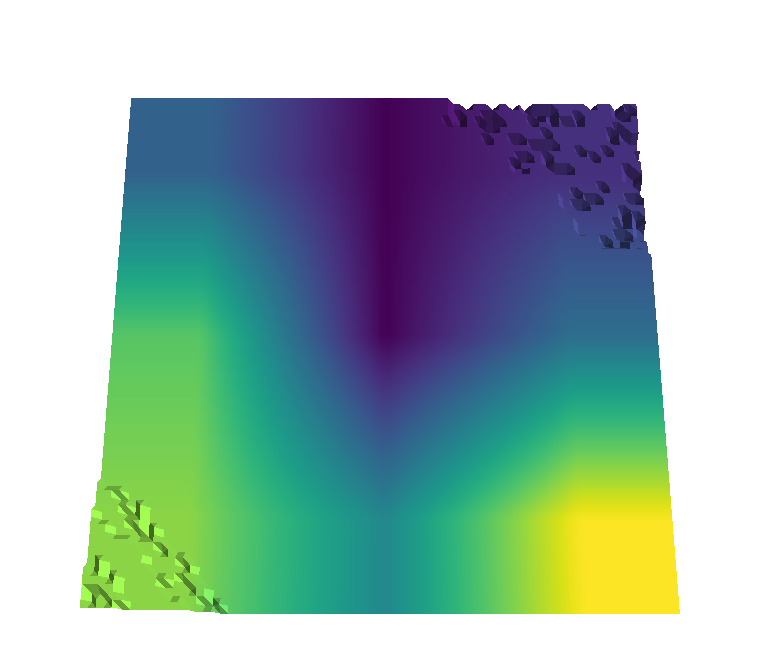
\includegraphics[width=\linewidth]{../img/5/quarry/best/25-patch-3d-majavi-colormap-10.png}
    \caption{0.26cm}
    \label{fig : quarry-best-1}
    \end{subfigure}
    \begin{subfigure}[b]{0.192\linewidth}
    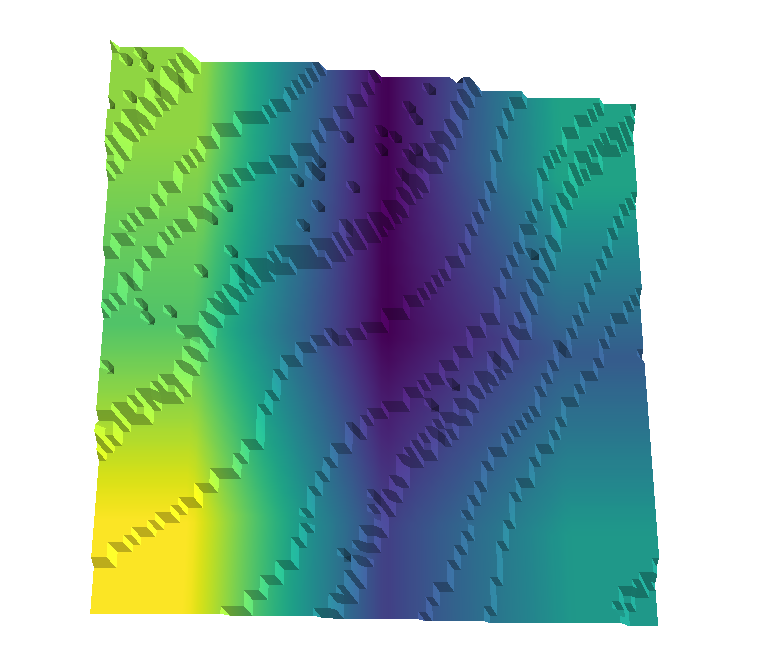
\includegraphics[width=\linewidth]{../img/5/quarry/best/30-patch-3d-majavi-colormap-20.png}
    \caption{0.30cm}
    \label{fig : quarry-best-2}
    \end{subfigure}
    \begin{subfigure}[b]{0.192\linewidth}
    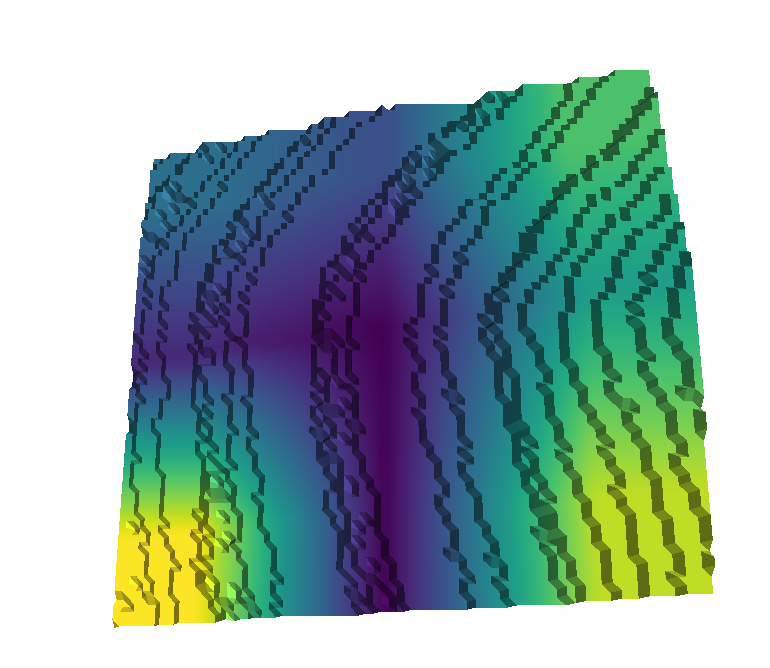
\includegraphics[width=\linewidth]{../img/5/quarry/best/34-patch-3d-majavi-colormap-30.png}
    \caption{0.35cm}
    \label{fig : quarry-best-3}
    \end{subfigure}
    \begin{subfigure}[b]{0.192\linewidth}
    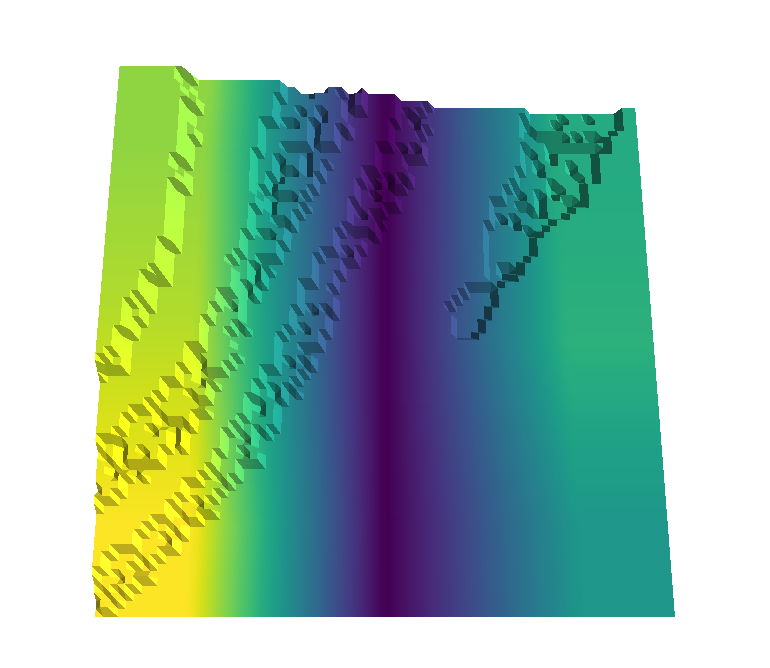
\includegraphics[width=\linewidth]{../img/5/quarry/best/38-patch-3d-majavi-colormap-40.png}
    \caption{0.38cm}
    \label{fig : quarry-best-4}
    \end{subfigure}
    \begin{subfigure}[b]{0.192\linewidth}
    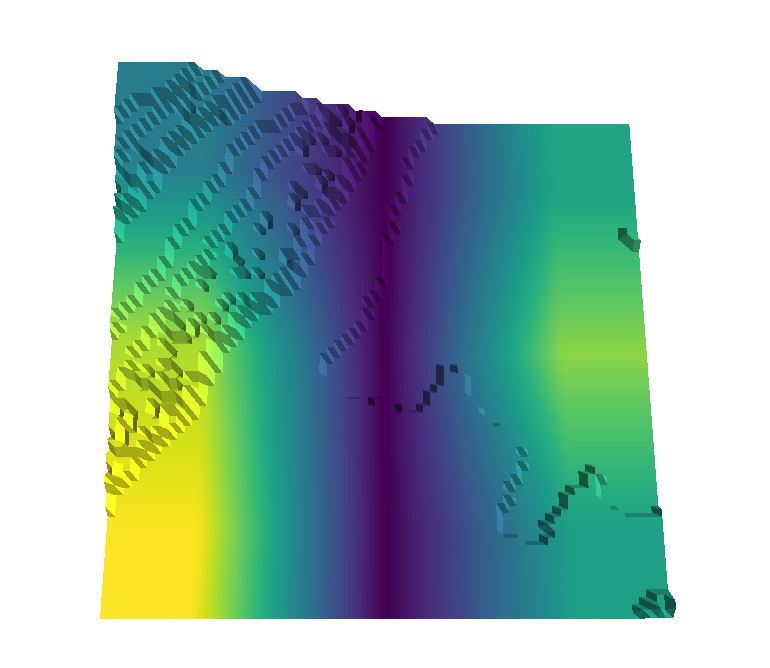
\includegraphics[width=\linewidth]{../img/5/quarry/best/41-patch-3d-majavi-colormap-50.png}
    \caption{0.41cm}
    \label{fig : quarry-best-5}
    \end{subfigure}
    \begin{subfigure}[b]{0.192\linewidth}
    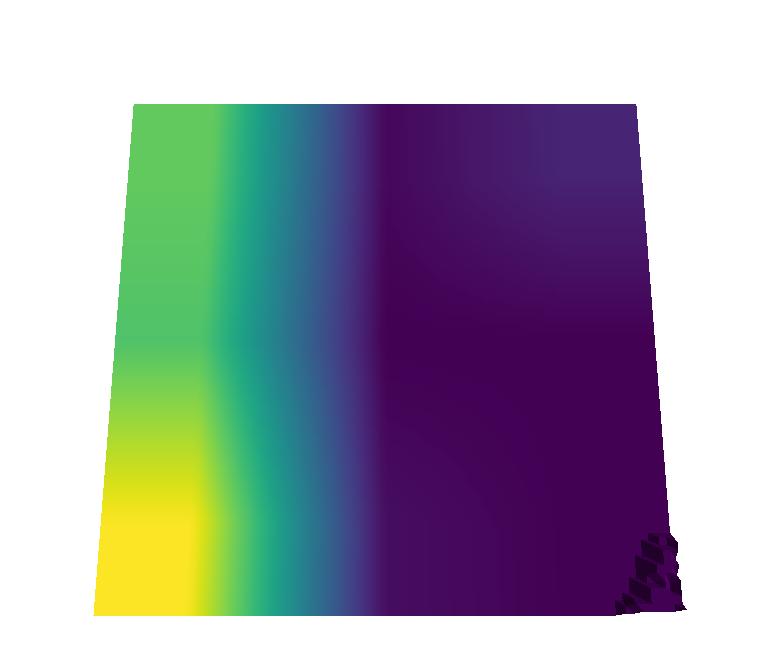
\includegraphics[width=\linewidth]{../img/5/quarry/best/44-patch-3d-majavi-colormap-60.png}
    \caption{0.44cm}
    \label{fig : quarry-best-6}
    \end{subfigure}
    \begin{subfigure}[b]{0.192\linewidth}
    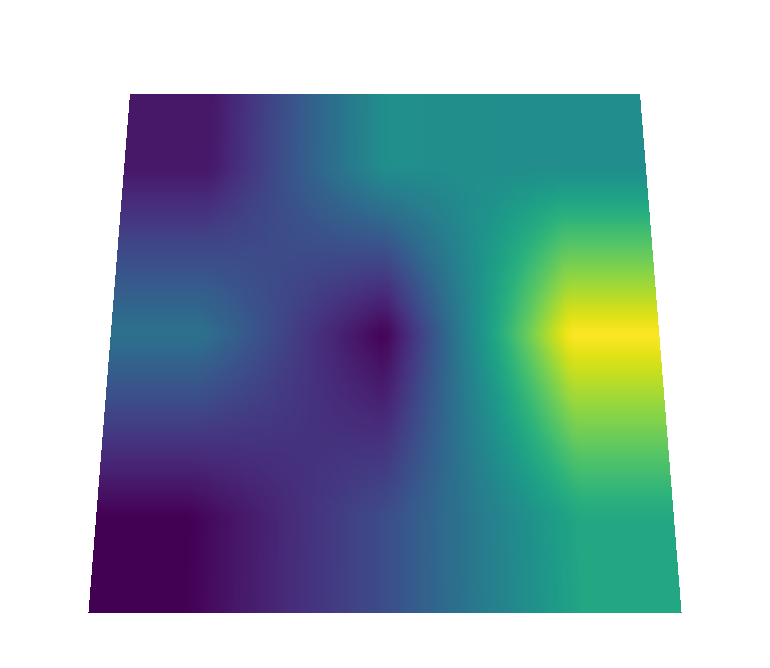
\includegraphics[width=\linewidth]{../img/5/quarry/best/46-patch-3d-majavi-colormap-70.png}
    \caption{0.47cm}
    \label{fig : quarry-best-7}
    \end{subfigure}
    \begin{subfigure}[b]{0.192\linewidth}
    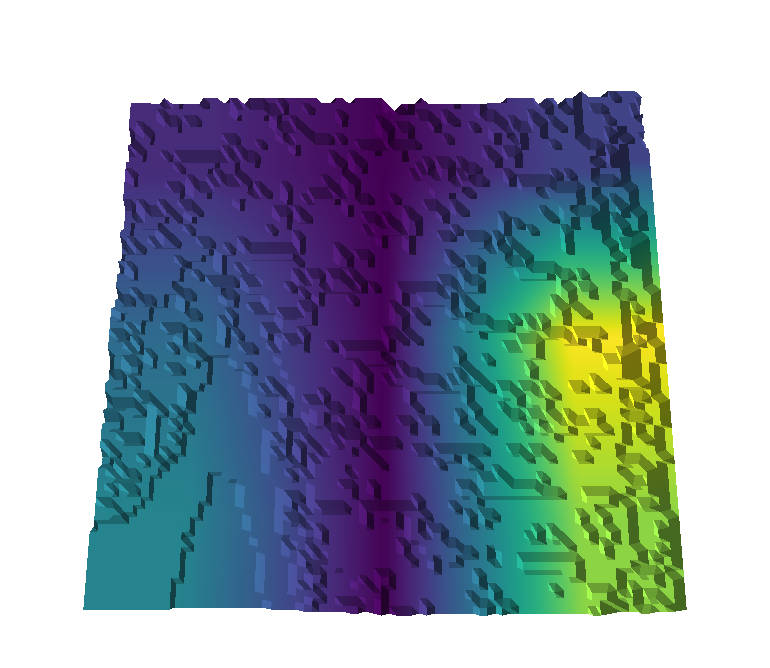
\includegraphics[width=\linewidth]{../img/5/quarry/best/49-patch-3d-majavi-colormap-80.png}
    \caption{0.49cm}
    \label{fig : quarry-best-8}
    \end{subfigure}
    \begin{subfigure}[b]{0.192\linewidth}
    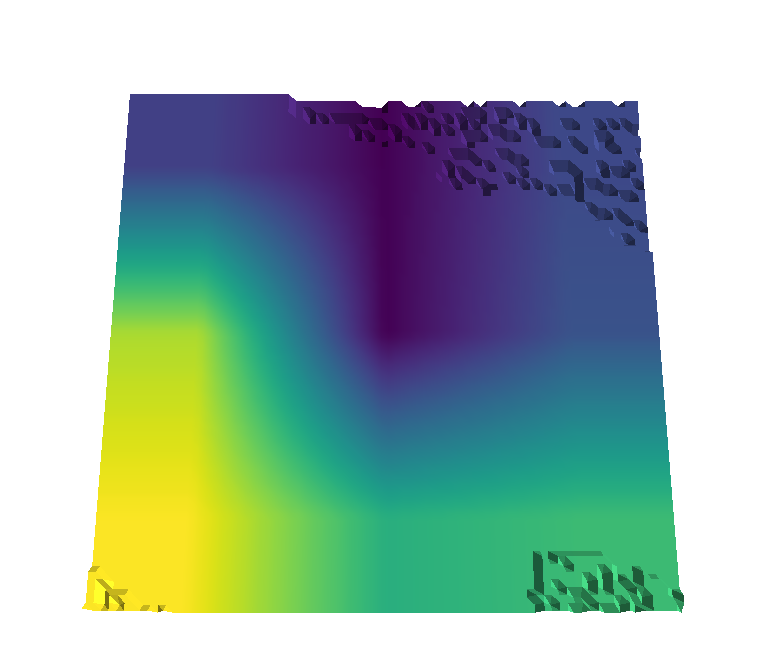
\includegraphics[width=\linewidth]{../img/5/quarry/best/51-patch-3d-majavi-colormap-90.png}
    \caption{0.52cm}
    \label{fig : quarry-best-9}
    \end{subfigure}
    \begin{subfigure}[b]{0.192\linewidth}
    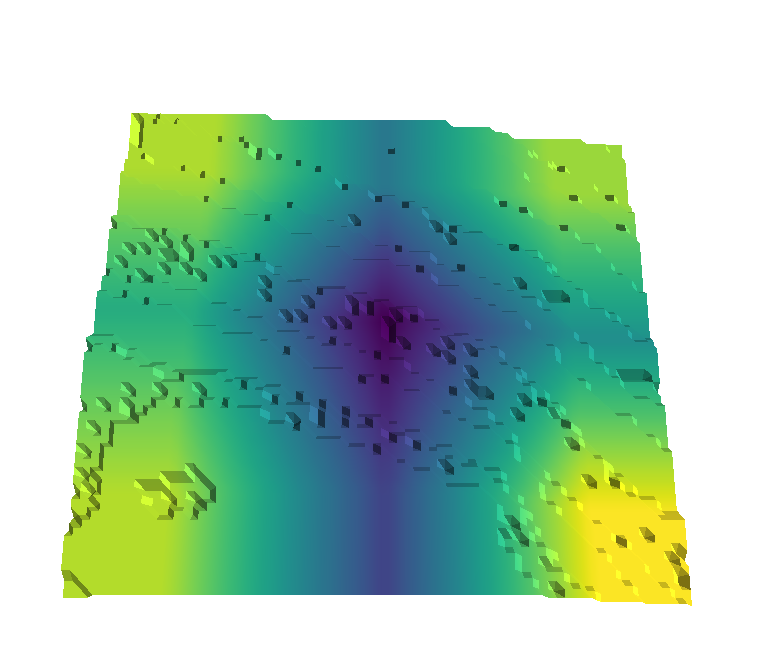
\includegraphics[width=\linewidth]{../img/5/quarry/best/54-patch-3d-majavi-colormap-100.png}
    \caption{0.54cm}
    \label{fig : quarry-best-10}
    \end{subfigure}
    \begin{subfigure}[b]{0.192\linewidth}
    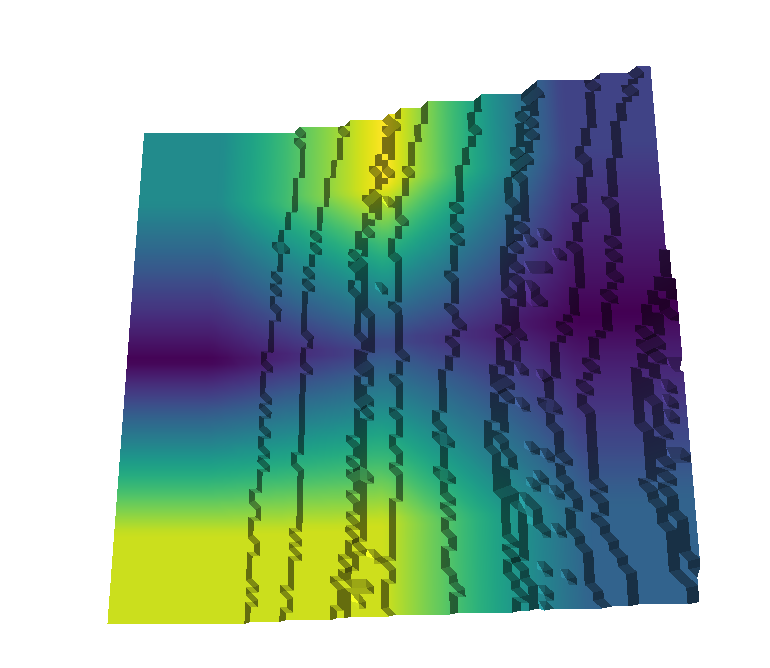
\includegraphics[width=\linewidth]{../img/5/quarry/best/56-patch-3d-majavi-colormap-110.png}
    \caption{0.57cm}
    \label{fig : quarry-best-11}
    \end{subfigure}
    \begin{subfigure}[b]{0.192\linewidth}
    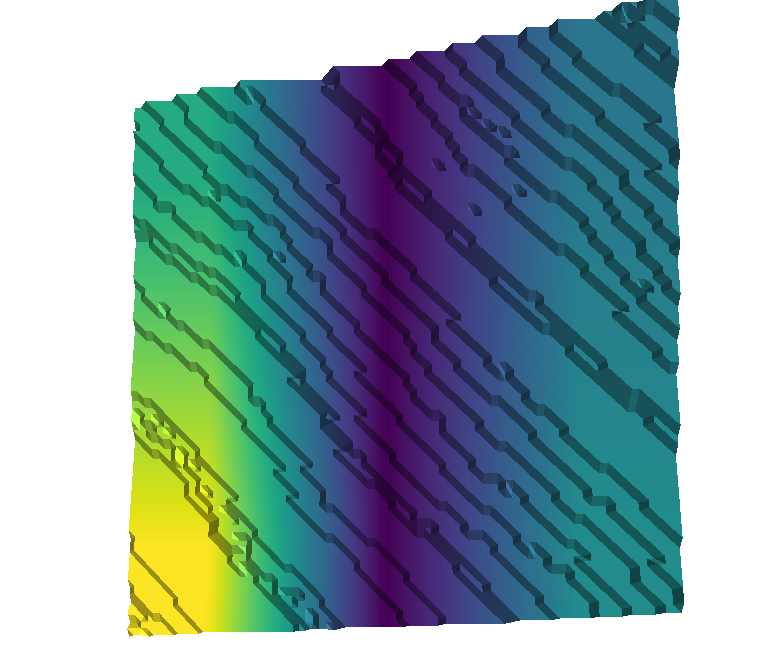
\includegraphics[width=\linewidth]{../img/5/quarry/best/58-patch-3d-majavi-colormap-120.png}
    \caption{0.59cm}
    \label{fig : quarry-best-12}
    \end{subfigure}
    \begin{subfigure}[b]{0.192\linewidth}
    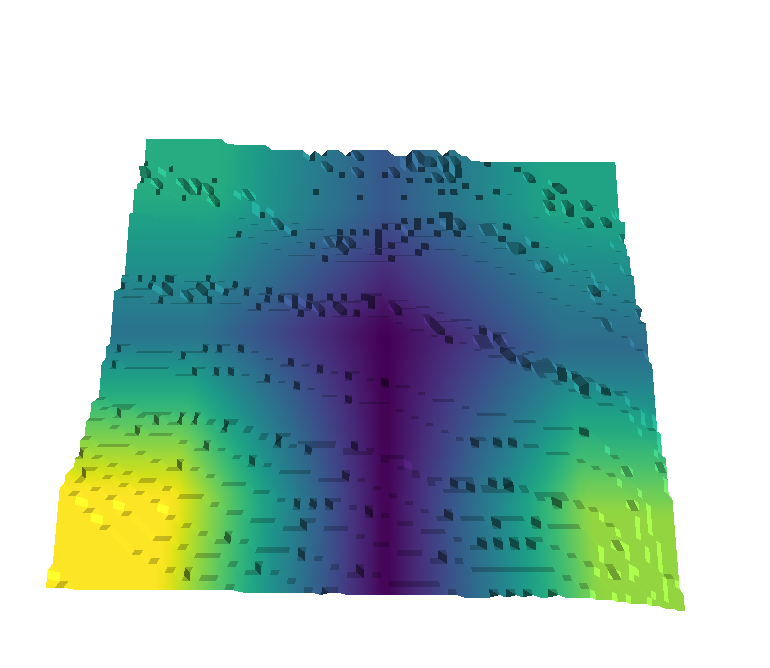
\includegraphics[width=\linewidth]{../img/5/quarry/best/60-patch-3d-majavi-colormap-130.png}
    \caption{0.60cm}
    \label{fig : quarry-best-13}
    \end{subfigure}
    \begin{subfigure}[b]{0.192\linewidth}
    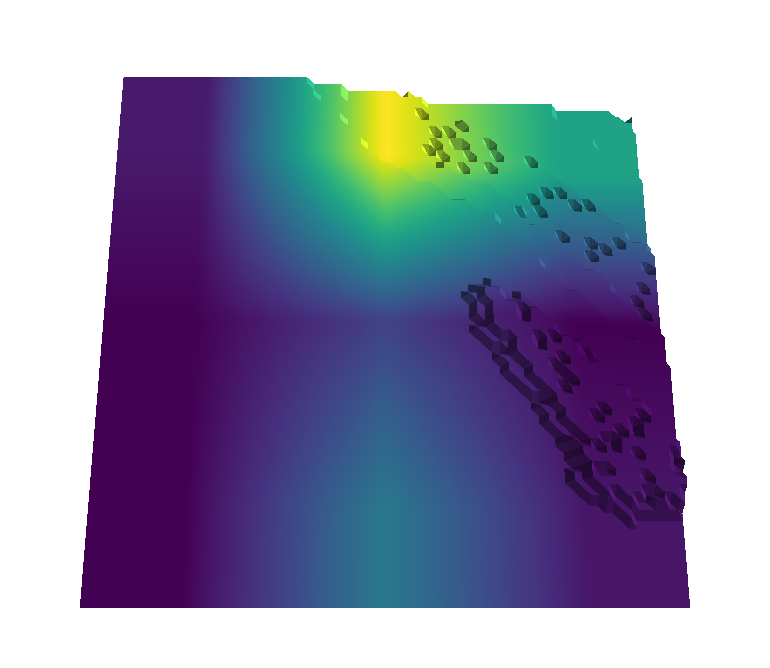
\includegraphics[width=\linewidth]{../img/5/quarry/best/62-patch-3d-majavi-colormap-140.png}
    \caption{0.62cm}
    \label{fig : quarry-best-14}
    \end{subfigure}
    \begin{subfigure}[b]{0.192\linewidth}
    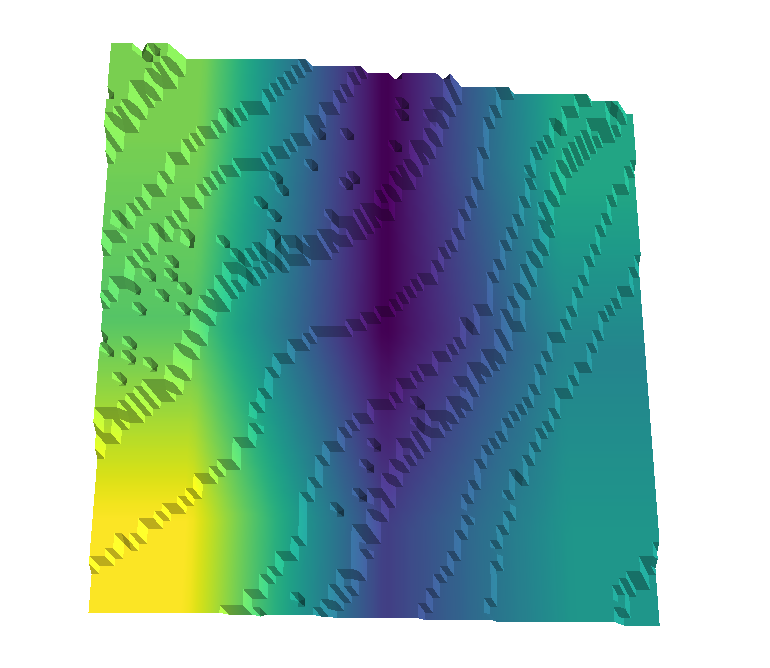
\includegraphics[width=\linewidth]{../img/5/quarry/best/63-patch-3d-majavi-colormap-150.png}
    \caption{0.64cm}
    \label{fig : quarry-best-15}
    \end{subfigure}
    \begin{subfigure}[b]{0.192\linewidth}
    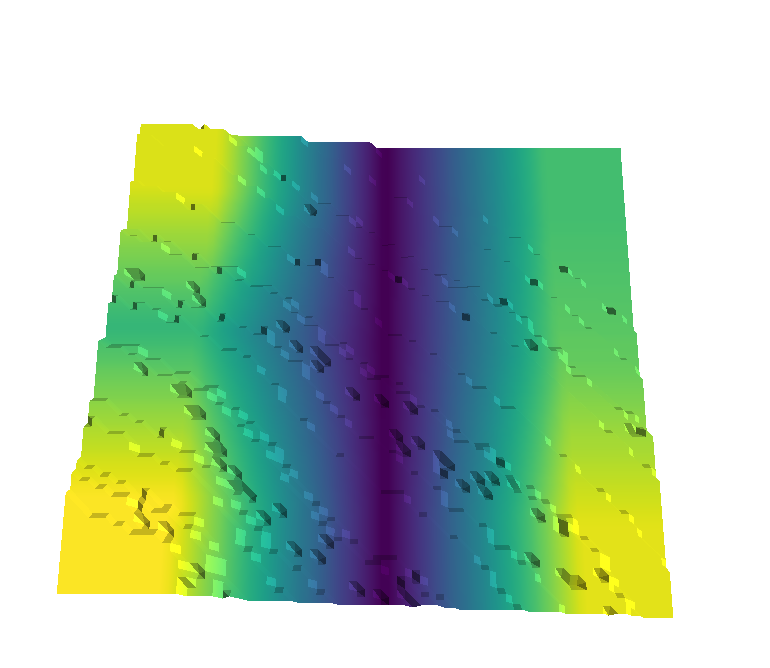
\includegraphics[width=\linewidth]{../img/5/quarry/best/65-patch-3d-majavi-colormap-160.png}
    \caption{0.66cm}
    \label{fig : quarry-best-16}
    \end{subfigure}
    \begin{subfigure}[b]{0.192\linewidth}
    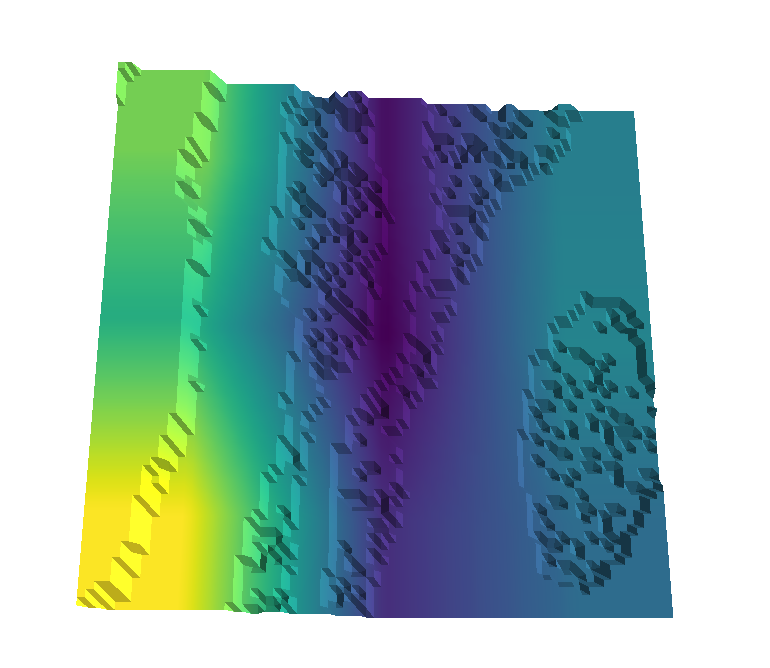
\includegraphics[width=\linewidth]{../img/5/quarry/best/67-patch-3d-majavi-colormap-170.png}
    \caption{0.67cm}
    \label{fig : quarry-best-17}
    \end{subfigure}
    \begin{subfigure}[b]{0.192\linewidth}
    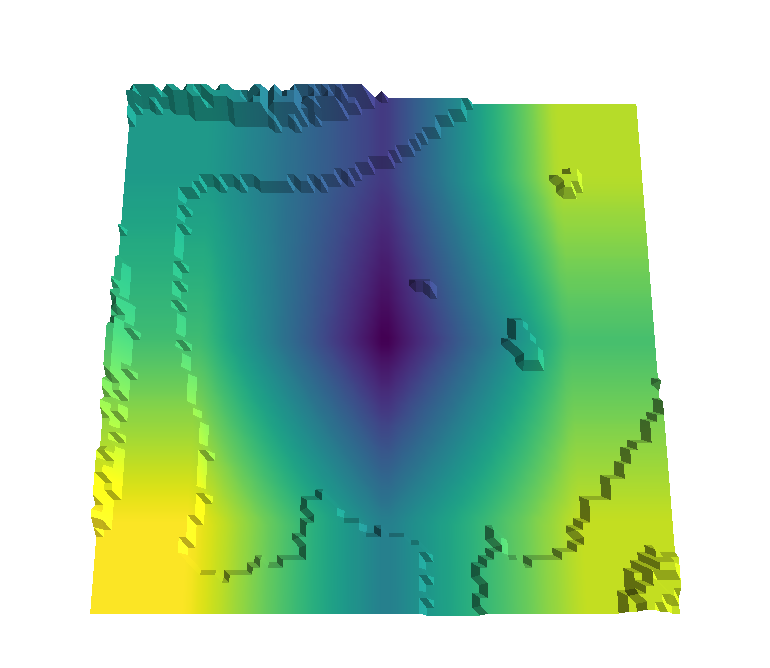
\includegraphics[width=\linewidth]{../img/5/quarry/best/68-patch-3d-majavi-colormap-180.png}
    \caption{0.68cm}
    \label{fig : quarry-best-18}
    \end{subfigure}
    \begin{subfigure}[b]{0.192\linewidth}
    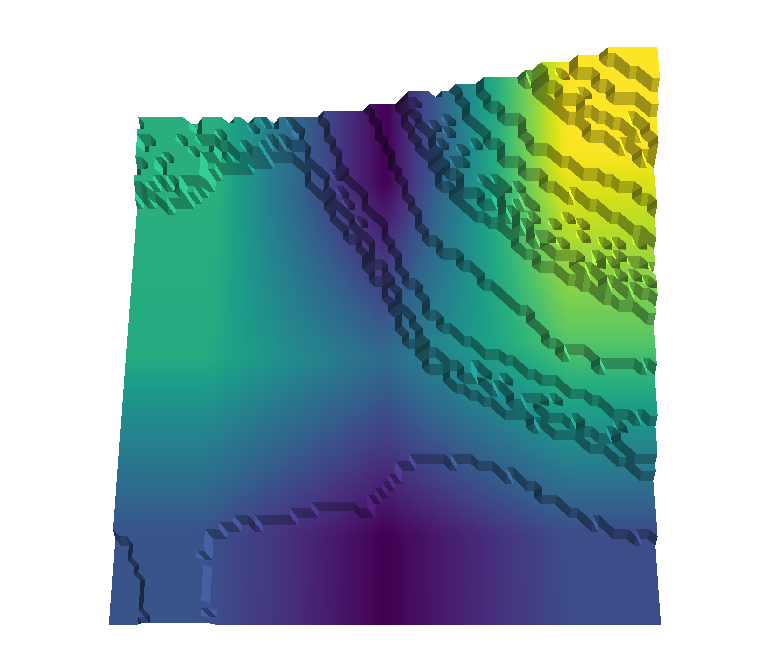
\includegraphics[width=\linewidth]{../img/5/quarry/best/70-patch-3d-majavi-colormap-190.png}
    \caption{0.70cm}
    \label{fig : quarry-best-19}
    \end{subfigure}
    \label{fig : quarry-best}
    \end{figure}

\subsection{Worst}
Those are the not traversable patches, we ordered by advancement. In this case, the region highlighted by the Grad-CAM are the features in the ground that contribute the most to make the patch not traversable. For instance, in some patches, \ref{fig : quarry-worst-1}, \ref{fig : quarry-worst-5}, \ref{fig : quarry-worst-19}, the most not traversable features is directly under the robot legs, similar as before. While, for the others samples, \ref{fig : quarry-worst-0}, \ref{fig : quarry-worst-2}, \ref{fig : quarry-worst-3}, \ref{fig : quarry-worst-4}, ..., the attention of the network is on the obstacles in front of the robot. This is oblious in  \ref{fig : quarry-worst-2}, \ref{fig : quarry-worst-2}, \ref{fig : quarry-worst-4}, where the big wall on the right is almost totally highlighted. So, also in this case, the model is able to understand which part of the patch cause the prediciton. 
\begin{figure}[H]
    \centering
    \begin{subfigure}[b]{0.192\linewidth}
    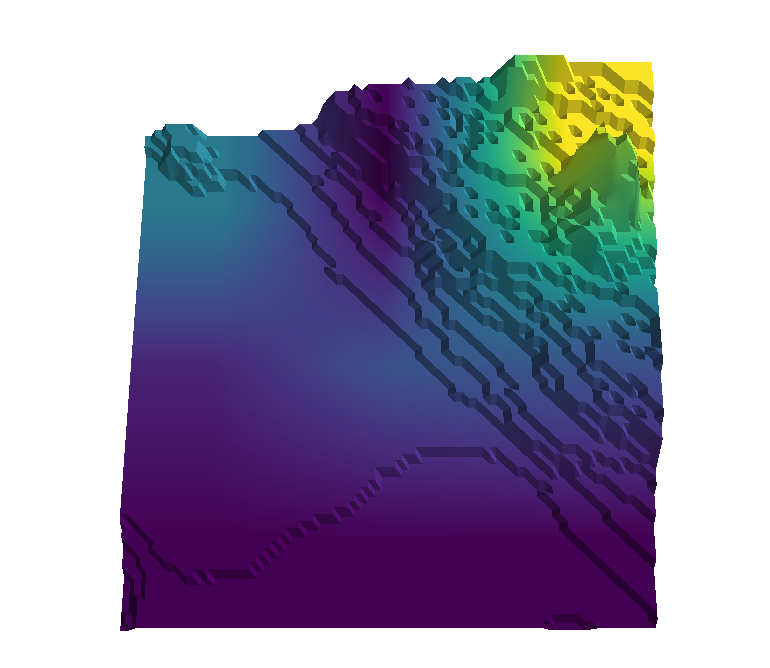
\includegraphics[width=\linewidth]{../img/5/quarry/worst/-35-patch-3d-majavi-colormap-0.png}
    \caption{-0.36cm}
    \label{fig : quarry-worst-0}
    \end{subfigure}
    \begin{subfigure}[b]{0.192\linewidth}
    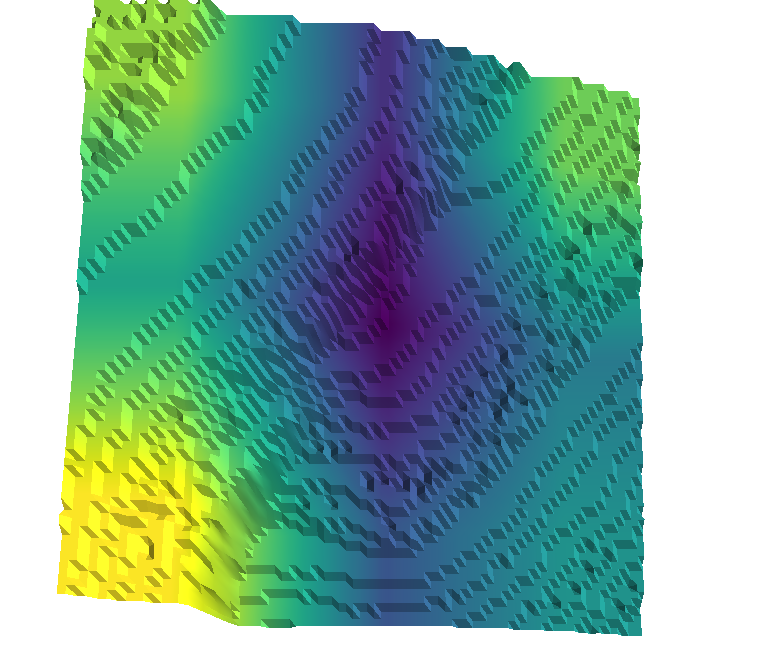
\includegraphics[width=\linewidth]{../img/5/quarry/worst/-7-patch-3d-majavi-colormap-10.png}
    \caption{-0.08cm}
    \label{fig : quarry-worst-1}
    \end{subfigure}
    \begin{subfigure}[b]{0.192\linewidth}
    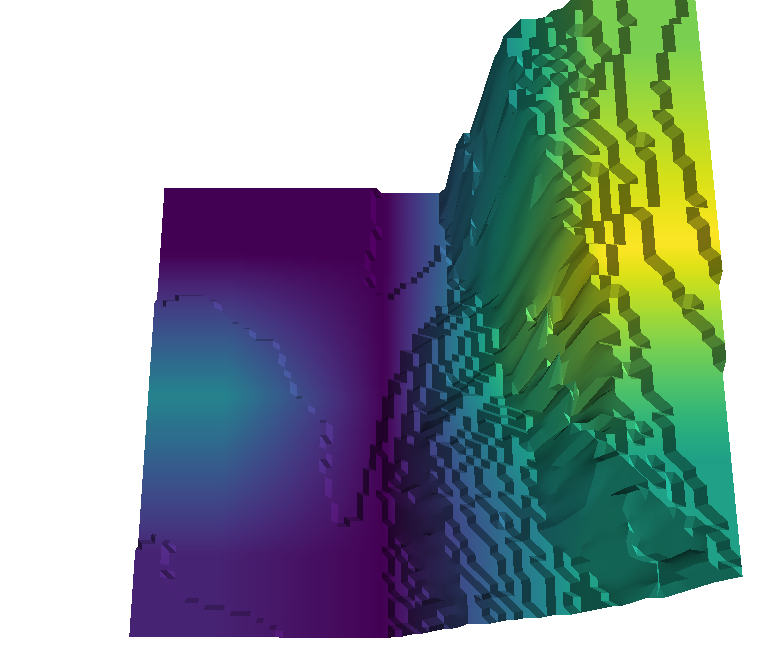
\includegraphics[width=\linewidth]{../img/5/quarry/worst/-4-patch-3d-majavi-colormap-20.png}
    \caption{-0.05cm}
    \label{fig : quarry-worst-2}
    \end{subfigure}
    \begin{subfigure}[b]{0.192\linewidth}
    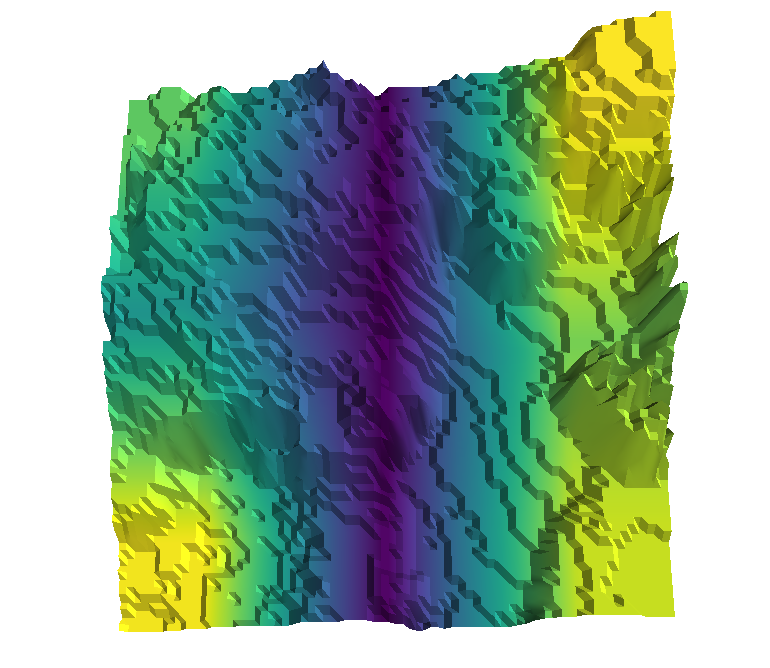
\includegraphics[width=\linewidth]{../img/5/quarry/worst/-3-patch-3d-majavi-colormap-30.png}
    \caption{-0.03cm}
    \label{fig : quarry-worst-3}
    \end{subfigure}
    \begin{subfigure}[b]{0.192\linewidth}
    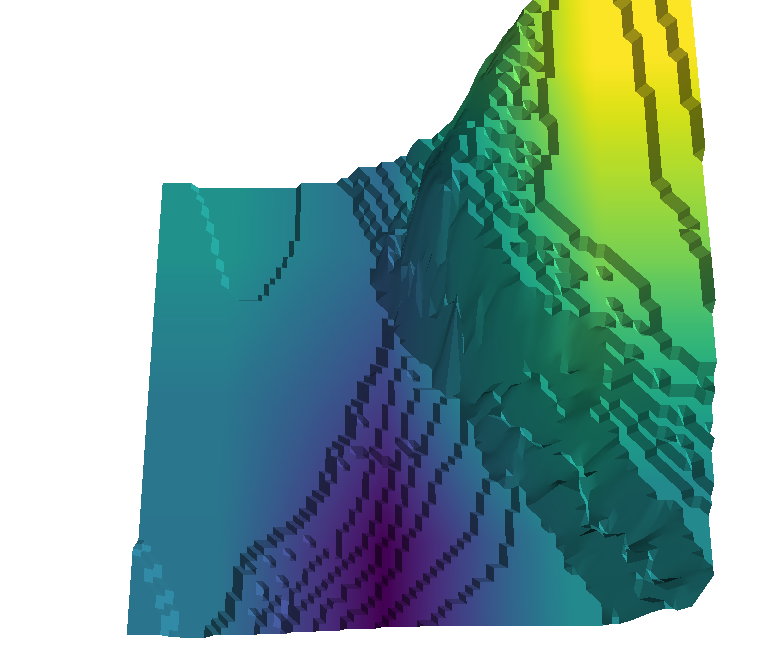
\includegraphics[width=\linewidth]{../img/5/quarry/worst/-2-patch-3d-majavi-colormap-40.png}
    \caption{-0.02cm}
    \label{fig : quarry-worst-4}
    \end{subfigure}
    \begin{subfigure}[b]{0.192\linewidth}
    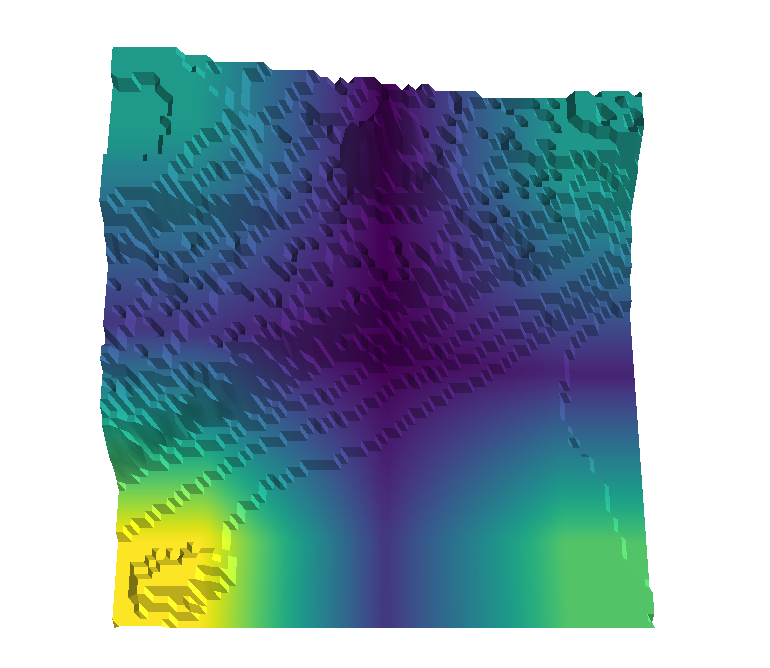
\includegraphics[width=\linewidth]{../img/5/quarry/worst/-1-patch-3d-majavi-colormap-50.png}
    \caption{-0.01cm}
    \label{fig : quarry-worst-5}
    \end{subfigure}
    \begin{subfigure}[b]{0.192\linewidth}
    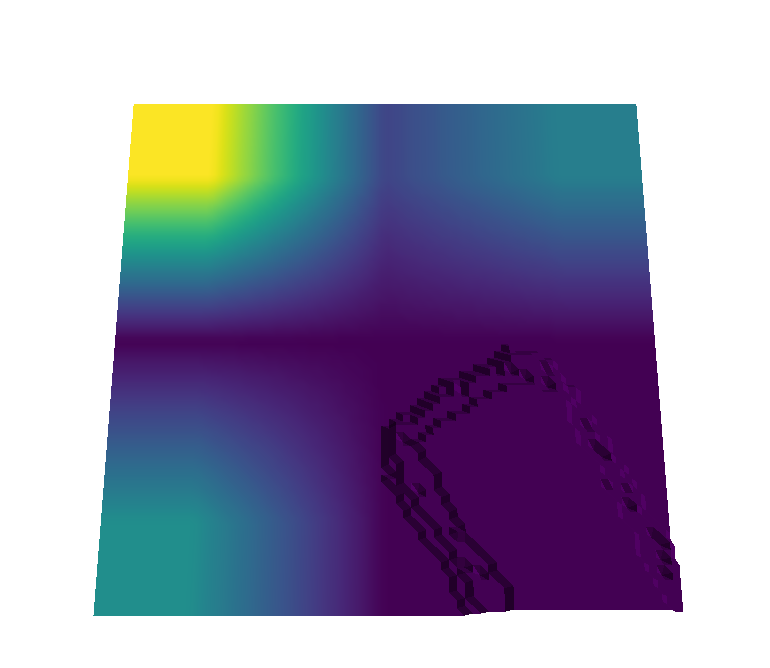
\includegraphics[width=\linewidth]{../img/5/quarry/worst/00-patch-3d-majavi-colormap-60.png}
    \caption{-0.01cm}
    \label{fig : quarry-worst-6}
    \end{subfigure}
    \begin{subfigure}[b]{0.192\linewidth}
    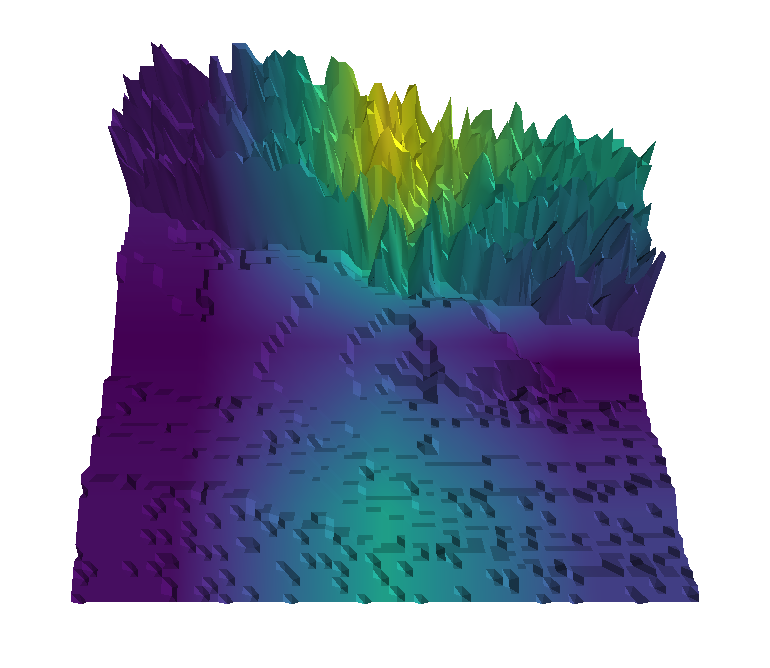
\includegraphics[width=\linewidth]{../img/5/quarry/worst/00-patch-3d-majavi-colormap-70.png}
    \caption{0.00cm}
    \label{fig : quarry-worst-7}
    \end{subfigure}
    \begin{subfigure}[b]{0.192\linewidth}
    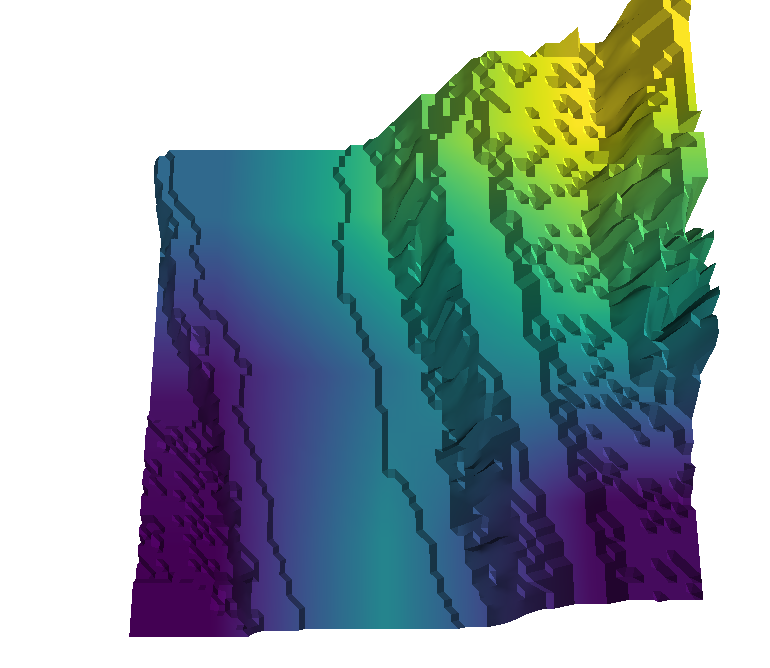
\includegraphics[width=\linewidth]{../img/5/quarry/worst/00-patch-3d-majavi-colormap-80.png}
    \caption{0.01cm}
    \label{fig : quarry-worst-8}
    \end{subfigure}
    \begin{subfigure}[b]{0.192\linewidth}
    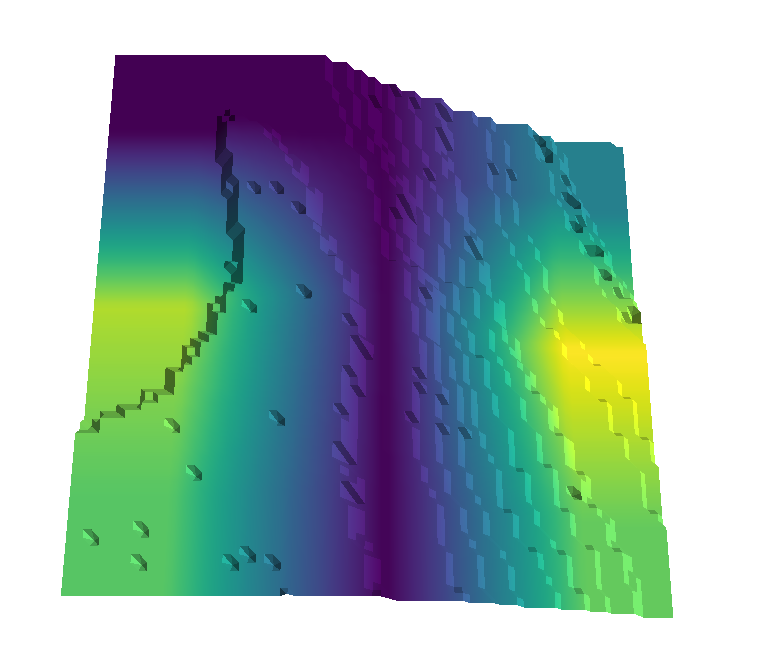
\includegraphics[width=\linewidth]{../img/5/quarry/worst/01-patch-3d-majavi-colormap-90.png}
    \caption{0.02cm}
    \label{fig : quarry-worst-9}
    \end{subfigure}
    \begin{subfigure}[b]{0.192\linewidth}
    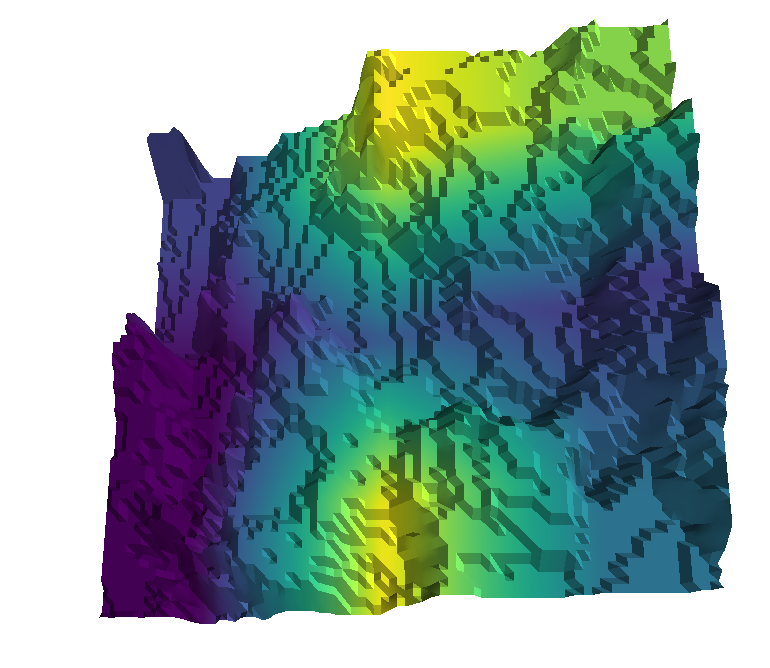
\includegraphics[width=\linewidth]{../img/5/quarry/worst/02-patch-3d-majavi-colormap-100.png}
    \caption{0.02cm}
    \label{fig : quarry-worst-10}
    \end{subfigure}
    \begin{subfigure}[b]{0.192\linewidth}
    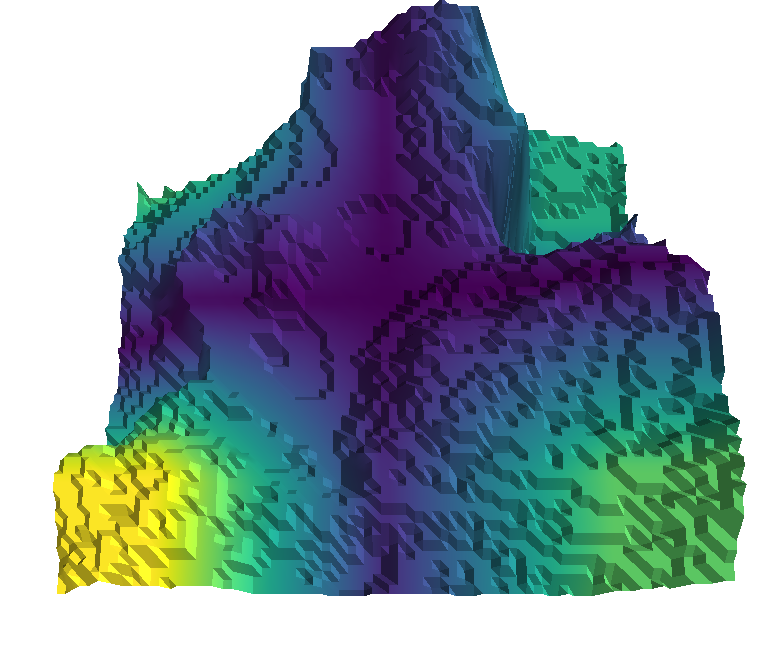
\includegraphics[width=\linewidth]{../img/5/quarry/worst/03-patch-3d-majavi-colormap-110.png}
    \caption{0.03cm}
    \label{fig : quarry-worst-11}
    \end{subfigure}
    \begin{subfigure}[b]{0.192\linewidth}
    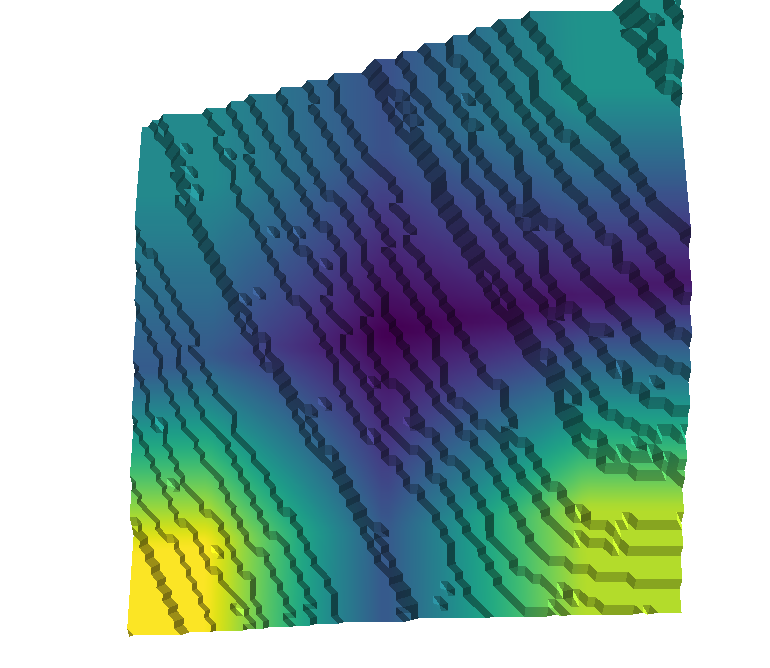
\includegraphics[width=\linewidth]{../img/5/quarry/worst/04-patch-3d-majavi-colormap-120.png}
    \caption{0.05cm}
    \label{fig : quarry-worst-12}
    \end{subfigure}
    \begin{subfigure}[b]{0.192\linewidth}
    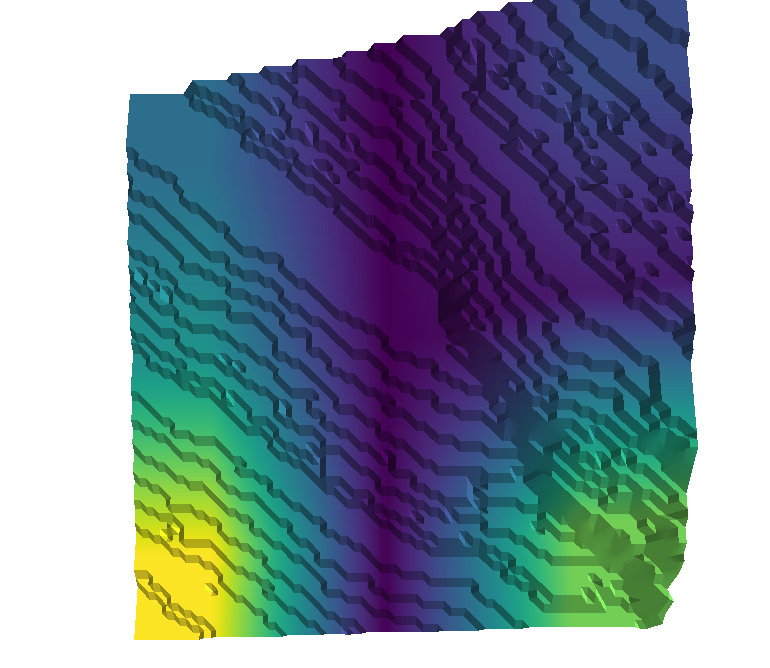
\includegraphics[width=\linewidth]{../img/5/quarry/worst/06-patch-3d-majavi-colormap-130.png}
    \caption{0.06cm}
    \label{fig : quarry-worst-13}
    \end{subfigure}
    \begin{subfigure}[b]{0.192\linewidth}
    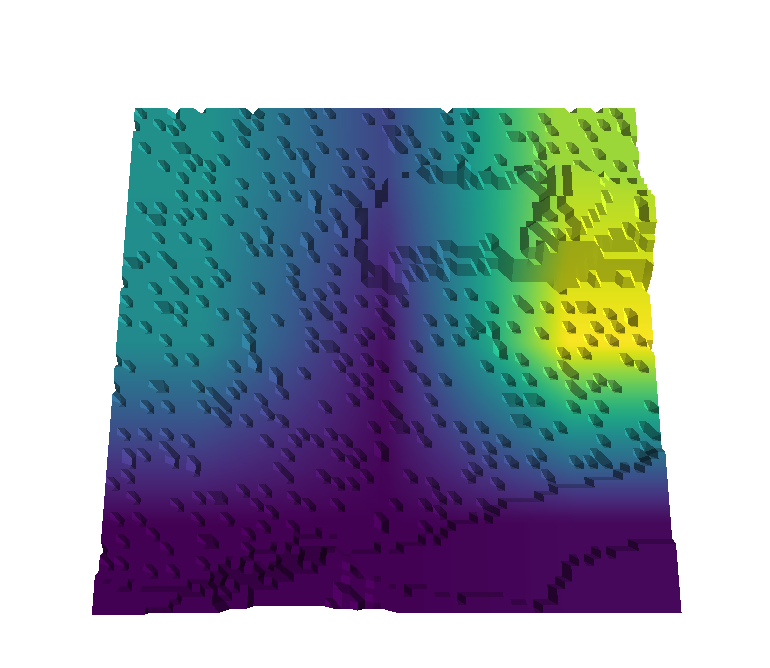
\includegraphics[width=\linewidth]{../img/5/quarry/worst/07-patch-3d-majavi-colormap-140.png}
    \caption{0.08cm}
    \label{fig : quarry-worst-14}
    \end{subfigure}
    \begin{subfigure}[b]{0.192\linewidth}
    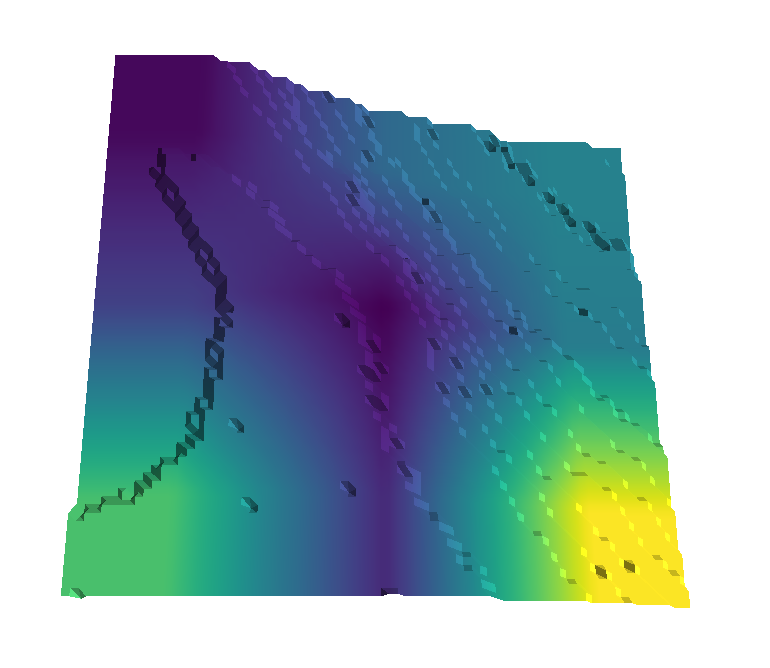
\includegraphics[width=\linewidth]{../img/5/quarry/worst/09-patch-3d-majavi-colormap-150.png}
    \caption{0.10cm}
    \label{fig : quarry-worst-15}
    \end{subfigure}
    \begin{subfigure}[b]{0.192\linewidth}
    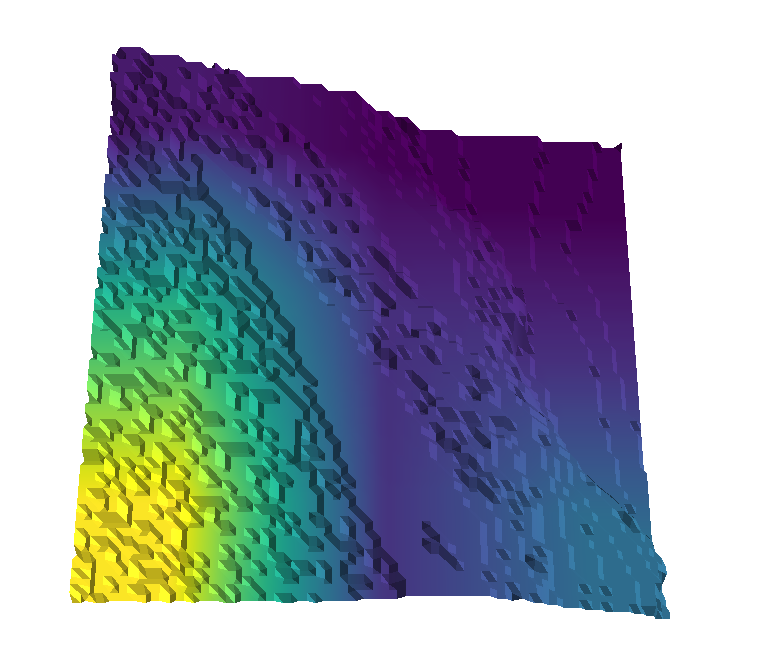
\includegraphics[width=\linewidth]{../img/5/quarry/worst/11-patch-3d-majavi-colormap-160.png}
    \caption{0.11cm}
    \label{fig : quarry-worst-16}
    \end{subfigure}
    \begin{subfigure}[b]{0.192\linewidth}
    \includegraphics[width=\linewidth]{../img/5/quarry/worst/13-patch-3d-majavi-colormap-170.png}
    \caption{0.13cm}
    \label{fig : quarry-worst-17}
    \end{subfigure}
    \begin{subfigure}[b]{0.192\linewidth}
    \includegraphics[width=\linewidth]{../img/5/quarry/worst/15-patch-3d-majavi-colormap-180.png}
    \caption{0.15cm}
    \label{fig : quarry-worst-18}
    \end{subfigure}
    \begin{subfigure}[b]{0.192\linewidth}
    \includegraphics[width=\linewidth]{../img/5/quarry/worst/17-patch-3d-majavi-colormap-190.png}
    \caption{0.17cm}
    \label{fig : quarry-worst-19}
    \end{subfigure}
    % \begin{subfigure}[b]{0.192\linewidth}
    % \includegraphics[width=\linewidth]{../img/5/quarry/worst/19-patch-3d-majavi-colormap-200.png}
    % \caption{0.20cm}
    % \label{fig : quarry-worst-20}
    % \end{subfigure}
    \label{fig : quarry-worst}
    \end{figure}

\subsection{False Negative}
Those are the inputs that were labeled as negative but predicted as positive. There are lots of interesting cases, we can cluster those patches in three groups: obstacles ahead, slopes and wall parallele to the robot. In figures \ref{fig : quarry-false_negative-0}, \ref{fig : quarry-false_negative-5}, \ref{fig : quarry-false_negative-13}, the models is looking at the obstacle in front of the robot.  Slopes, figures \ref{fig : quarry-false_negative-1}, \ref{fig : quarry-false_negative-8}, \ref{fig : quarry-false_negative-11}, \ref{fig : quarry-false_negative-14}, \ref{fig : quarry-false_negative-15}, \ref{fig : quarry-false_negative-19}, are not completely smooth, making harder to classify them. The last cluster of inputs are the ones with a wall parallel to the robot, figures \ref{fig : quarry-false_negative-13} and \ref{fig : quarry-false_negative-19}. In those cases the model looks at the initial position of the robot, left, and the final part of the patch. Intuitivelly, is trying to understand if the robot fits on the trail. 

In general, most of the region of interested on those patches are located on the left, close to the position of the robot's leg. Correctly, even if the prediction is wrong, the model looks at the first region of the surface, located near the legs, that can cause non traversability. This shown a correct behaviour even with wrongly prediciton meaning that the network is always looking in the correct spot. 
\begin{figure}[H]
\centering
\begin{subfigure}[b]{0.192\linewidth}
\includegraphics[width=\linewidth]{../img/5/quarry/false_negative/-14-patch-3d-majavi-colormap-0.png}
\caption{-0.14cm}
\label{fig : quarry-false_negative-0}
\end{subfigure}
\begin{subfigure}[b]{0.192\linewidth}
\includegraphics[width=\linewidth]{../img/5/quarry/false_negative/-6-patch-3d-majavi-colormap-10.png}
\caption{-0.07cm}
\label{fig : quarry-false_negative-1}
\end{subfigure}
\begin{subfigure}[b]{0.192\linewidth}
\includegraphics[width=\linewidth]{../img/5/quarry/false_negative/-4-patch-3d-majavi-colormap-20.png}
\caption{-0.05cm}
\label{fig : quarry-false_negative-2}
\end{subfigure}
\begin{subfigure}[b]{0.192\linewidth}
\includegraphics[width=\linewidth]{../img/5/quarry/false_negative/-2-patch-3d-majavi-colormap-30.png}
\caption{-0.02cm}
\label{fig : quarry-false_negative-3}
\end{subfigure}
\begin{subfigure}[b]{0.192\linewidth}
\includegraphics[width=\linewidth]{../img/5/quarry/false_negative/00-patch-3d-majavi-colormap-40.png}
\caption{-0.00cm}
\label{fig : quarry-false_negative-4}
\end{subfigure}
\begin{subfigure}[b]{0.192\linewidth}
\includegraphics[width=\linewidth]{../img/5/quarry/false_negative/01-patch-3d-majavi-colormap-50.png}
\caption{0.01cm}
\label{fig : quarry-false_negative-5}
\end{subfigure}
\begin{subfigure}[b]{0.192\linewidth}
\includegraphics[width=\linewidth]{../img/5/quarry/false_negative/02-patch-3d-majavi-colormap-60.png}
\caption{0.03cm}
\label{fig : quarry-false_negative-6}
\end{subfigure}
\begin{subfigure}[b]{0.192\linewidth}
\includegraphics[width=\linewidth]{../img/5/quarry/false_negative/04-patch-3d-majavi-colormap-70.png}
\caption{0.04cm}
\label{fig : quarry-false_negative-7}
\end{subfigure}
\begin{subfigure}[b]{0.192\linewidth}
\includegraphics[width=\linewidth]{../img/5/quarry/false_negative/05-patch-3d-majavi-colormap-80.png}
\caption{0.06cm}
\label{fig : quarry-false_negative-8}
\end{subfigure}
\begin{subfigure}[b]{0.192\linewidth}
\includegraphics[width=\linewidth]{../img/5/quarry/false_negative/06-patch-3d-majavi-colormap-90.png}
\caption{0.07cm}
\label{fig : quarry-false_negative-9}
\end{subfigure}
\begin{subfigure}[b]{0.192\linewidth}
\includegraphics[width=\linewidth]{../img/5/quarry/false_negative/08-patch-3d-majavi-colormap-100.png}
\caption{0.08cm}
\label{fig : quarry-false_negative-10}
\end{subfigure}
\begin{subfigure}[b]{0.192\linewidth}
\includegraphics[width=\linewidth]{../img/5/quarry/false_negative/09-patch-3d-majavi-colormap-110.png}
\caption{0.09cm}
\label{fig : quarry-false_negative-11}
\end{subfigure}
\begin{subfigure}[b]{0.192\linewidth}
\includegraphics[width=\linewidth]{../img/5/quarry/false_negative/10-patch-3d-majavi-colormap-120.png}
\caption{0.11cm}
\label{fig : quarry-false_negative-12}
\end{subfigure}
\begin{subfigure}[b]{0.192\linewidth}
\includegraphics[width=\linewidth]{../img/5/quarry/false_negative/11-patch-3d-majavi-colormap-130.png}
\caption{0.12cm}
\label{fig : quarry-false_negative-13}
\end{subfigure}
\begin{subfigure}[b]{0.192\linewidth}
\includegraphics[width=\linewidth]{../img/5/quarry/false_negative/12-patch-3d-majavi-colormap-140.png}
\caption{0.13cm}
\label{fig : quarry-false_negative-14}
\end{subfigure}
\begin{subfigure}[b]{0.192\linewidth}
\includegraphics[width=\linewidth]{../img/5/quarry/false_negative/14-patch-3d-majavi-colormap-150.png}
\caption{0.14cm}
\label{fig : quarry-false_negative-15}
\end{subfigure}
\begin{subfigure}[b]{0.192\linewidth}
\includegraphics[width=\linewidth]{../img/5/quarry/false_negative/15-patch-3d-majavi-colormap-160.png}
\caption{0.15cm}
\label{fig : quarry-false_negative-16}
\end{subfigure}
\begin{subfigure}[b]{0.192\linewidth}
\includegraphics[width=\linewidth]{../img/5/quarry/false_negative/16-patch-3d-majavi-colormap-170.png}
\caption{0.17cm}
\label{fig : quarry-false_negative-17}
\end{subfigure}
\begin{subfigure}[b]{0.192\linewidth}
\includegraphics[width=\linewidth]{../img/5/quarry/false_negative/17-patch-3d-majavi-colormap-180.png}
\caption{0.18cm}
\label{fig : quarry-false_negative-18}
\end{subfigure}
\begin{subfigure}[b]{0.192\linewidth}
\includegraphics[width=\linewidth]{../img/5/quarry/false_negative/18-patch-3d-majavi-colormap-190.png}
\caption{0.18cm}
\label{fig : quarry-false_negative-19}
\end{subfigure}
% \begin{subfigure}[b]{0.192\linewidth}
% \includegraphics[width=\linewidth]{../img/5/quarry/false_negative/19-patch-3d-majavi-colormap-200.png}
% \caption{0.19cm}
% \label{fig : quarry-false_negative-20}
% \end{subfigure}
\label{fig : quarry-false_negative}
\end{figure}

\subsection{False Positive}
Those are the most interesting ones, they are the samples that were labeled as traversable but predicted as not traversable. They includes different types of patches, obstacles ahead, slopes and flat regions. In each case the model looks at meaningfull features in the patches that can effect traversability. In the slopes, \ref{fig : quarry-false_positive-8} and \ref{false_positive-9}, the first part of the surface is highlighted. Similar as before, the model is looking if the rear legs will be able to move and thought that those small steps will cause the robot not advance enough. The same consideration can be done for figure \ref{fig : quarry-false_positive-5}. On the other hand, some inputs. definitely confused the model. For instance, in figures \ref{fig : quarry-false_positive-7} and \ref{fig : quarry-false_positive-18} the model is more interested in the big obstacle on the right part. This lead to classify those patches as not traversable, even if the obstacle is more distant than the treshold, in this case the network was totally confused. Interesting, figure \ref{fig : quarry-false_positive-13} shows an almost identical situation in which the network correctly looks at the initial part of the ground. We can deduce that even if the in almost any cases the network's prediction is caused by the correct part of the inputs, it can be confused by big obstacle near the end.
\begin{figure}[H]
    \centering
    \begin{subfigure}[b]{0.192\linewidth}
    \includegraphics[width=\linewidth]{../img/5/quarry/false_positive/20-patch-3d-majavi-colormap-0.png}
    \caption{0.20cm}
    \label{fig : quarry-false_positive-0}
    \end{subfigure}
    \begin{subfigure}[b]{0.192\linewidth}
    \includegraphics[width=\linewidth]{../img/5/quarry/false_positive/20-patch-3d-majavi-colormap-12.png}
    \caption{0.21cm}
    \label{fig : quarry-false_positive-1}
    \end{subfigure}
    \begin{subfigure}[b]{0.192\linewidth}
    \includegraphics[width=\linewidth]{../img/5/quarry/false_positive/22-patch-3d-majavi-colormap-24.png}
    \caption{0.22cm}
    \label{fig : quarry-false_positive-2}
    \end{subfigure}
    \begin{subfigure}[b]{0.192\linewidth}
    \includegraphics[width=\linewidth]{../img/5/quarry/false_positive/23-patch-3d-majavi-colormap-36.png}
    \caption{0.23cm}
    \label{fig : quarry-false_positive-3}
    \end{subfigure}
    \begin{subfigure}[b]{0.192\linewidth}
    \includegraphics[width=\linewidth]{../img/5/quarry/false_positive/24-patch-3d-majavi-colormap-48.png}
    \caption{0.24cm}
    \label{fig : quarry-false_positive-4}
    \end{subfigure}
    \begin{subfigure}[b]{0.192\linewidth}
    \includegraphics[width=\linewidth]{../img/5/quarry/false_positive/25-patch-3d-majavi-colormap-60.png}
    \caption{0.25cm}
    \label{fig : quarry-false_positive-5}
    \end{subfigure}
    \begin{subfigure}[b]{0.192\linewidth}
    \includegraphics[width=\linewidth]{../img/5/quarry/false_positive/25-patch-3d-majavi-colormap-72.png}
    \caption{0.26cm}
    \label{fig : quarry-false_positive-6}
    \end{subfigure}
    \begin{subfigure}[b]{0.192\linewidth}
    \includegraphics[width=\linewidth]{../img/5/quarry/false_positive/26-patch-3d-majavi-colormap-84.png}
    \caption{0.27cm}
    \label{fig : quarry-false_positive-7}
    \end{subfigure}
    \begin{subfigure}[b]{0.192\linewidth}
    \includegraphics[width=\linewidth]{../img/5/quarry/false_positive/27-patch-3d-majavi-colormap-96.png}
    \caption{0.27cm}
    \label{fig : quarry-false_positive-8}
    \end{subfigure}
    \begin{subfigure}[b]{0.192\linewidth}
    \includegraphics[width=\linewidth]{../img/5/quarry/false_positive/27-patch-3d-majavi-colormap-108.png}
    \caption{0.28cm}
    \label{fig : quarry-false_positive-9}
    \end{subfigure}
    \begin{subfigure}[b]{0.192\linewidth}
    \includegraphics[width=\linewidth]{../img/5/quarry/false_positive/29-patch-3d-majavi-colormap-120.png}
    \caption{0.29cm}
    \label{fig : quarry-false_positive-10}
    \end{subfigure}
    \begin{subfigure}[b]{0.192\linewidth}
    \includegraphics[width=\linewidth]{../img/5/quarry/false_positive/30-patch-3d-majavi-colormap-132.png}
    \caption{0.30cm}
    \label{fig : quarry-false_positive-11}
    \end{subfigure}
    \begin{subfigure}[b]{0.192\linewidth}
    \includegraphics[width=\linewidth]{../img/5/quarry/false_positive/31-patch-3d-majavi-colormap-144.png}
    \caption{0.32cm}
    \label{fig : quarry-false_positive-12}
    \end{subfigure}
    \begin{subfigure}[b]{0.192\linewidth}
    \includegraphics[width=\linewidth]{../img/5/quarry/false_positive/33-patch-3d-majavi-colormap-156.png}
    \caption{0.34cm}
    \label{fig : quarry-false_positive-13}
    \end{subfigure}
    \begin{subfigure}[b]{0.192\linewidth}
    \includegraphics[width=\linewidth]{../img/5/quarry/false_positive/35-patch-3d-majavi-colormap-168.png}
    \caption{0.35cm}
    \label{fig : quarry-false_positive-14}
    \end{subfigure}
    \begin{subfigure}[b]{0.192\linewidth}
    \includegraphics[width=\linewidth]{../img/5/quarry/false_positive/36-patch-3d-majavi-colormap-180.png}
    \caption{0.36cm}
    \label{fig : quarry-false_positive-15}
    \end{subfigure}
    \begin{subfigure}[b]{0.192\linewidth}
    \includegraphics[width=\linewidth]{../img/5/quarry/false_positive/38-patch-3d-majavi-colormap-192.png}
    \caption{0.39cm}
    \label{fig : quarry-false_positive-16}
    \end{subfigure}
    \begin{subfigure}[b]{0.192\linewidth}
    \includegraphics[width=\linewidth]{../img/5/quarry/false_positive/41-patch-3d-majavi-colormap-204.png}
    \caption{0.41cm}
    \label{fig : quarry-false_positive-17}
    \end{subfigure}
    \begin{subfigure}[b]{0.192\linewidth}
    \includegraphics[width=\linewidth]{../img/5/quarry/false_positive/46-patch-3d-majavi-colormap-216.png}
    \caption{0.46cm}
    \label{fig : quarry-false_positive-18}
    \end{subfigure}
    \begin{subfigure}[b]{0.192\linewidth}
    \includegraphics[width=\linewidth]{../img/5/quarry/false_positive/51-patch-3d-majavi-colormap-228.png}
    \caption{0.52cm}
    \label{fig : quarry-false_positive-19}
    \end{subfigure}
    % \begin{subfigure}[b]{0.192\linewidth}
    % \includegraphics[width=\linewidth]{../img/5/quarry/false_positive/61-patch-3d-majavi-colormap-240.png}
    % \caption{0.62cm}
    % \label{fig : quarry-false_positive-20}
    % \end{subfigure}
    \label{fig : quarry-false_positive}
    \end{figure}


\end{document}
\documentclass[./chapter5.tex]{subfiles}
\begin{document}
\section{Robustness}


\end{document}
% %

\end{document}\documentclass[../document.tex]{subfiles}